\chapter{Calcolo Differenziale}

In questo capitolo sono trattate funzioni $f: A \to \R^m$ con $A \subseteq \R^n$, dove $r,m \in \N$ e $n,m \geq 1$.\\
Generalmente, effettuata una dimostrazione per $m = 1$ è abbastanza semplice passare ad un $m > 1$ \textit{affiancando} le componenti, mentre non è altrettanto triviale il passaggio a $n > 1$.

\section{Preliminari}
In $\R^n$ verranno usate le (note) strutture vettoriale con la metrica Euclidea di \hyperref[ex:dist_eucl]{\cref*{ex:metriche} (\nameref*{ex:metriche})} % NOTE The \fullref command was not used on purpose to point this link straight to the right part of the aforementioned exercise

La base canonica di $R^n$ è indicata con $(e_1,\:\dotsc\:,e_n)$, $e_i$ è il vettore di $R^n$ con tutte le componenti nulle tranne la i-esima che vale 1. È dunque possibile scrivere un generico vettore $x$ si può quindi scrivere come combinazione lineare dei vettori della base canonica $x=\sum\limits_{i=1}^{n} x_i e_i$.

Nel caso $n=2$ è usata la notazione $(x,y)=xi+yj$. Nel caso $n=3$ è usata la notazione $(x,y,z)=xi+yj+zk$

Alcune classi di funzioni $f:A\subseteq\R^n \to\R^m$ hanno nomi particolari:
\begin{itemize}
	\item $n=1$,$m=1$: $f$ è una \textit{funzione reale di una variabile reale};
	\item $n=1$,$m>1$: $f$ è una \textit{curva} in $R^m$ (purché $f$ sia almeno continua e $A$ su un intervallo)
	\item $n>1$,$m=1$: $f$ è un \textit{campo scalare}
	\item $n>1$,$m>1$: $f$ è un \textit{campo vettoriale} (soprattutto nei casi $n=m=2$ e $n=m=3$)
\end{itemize}

\newpage
\section{Derivate Parziali e Direzionali}
Direttamente dalla nozione di Analisi 1 di derivata, cioè
\begin{align*}
	f'(x_0) = \lim\limits_{t \to 0} \frac{f(x_0 + t) - f(x_0)}{t} \tag{\textbf{NB}. Analisi 1!}
\end{align*}
si estende il concetto di derivata alle funzioni in spazi $n$\textit{-dimensionali} mediante la seguente
\begin{definition}[Derivata Direzionale e Parziale]
	\label{def:deriv_direz}
	Sia $A \subseteq \R^n$, $f: A \to \R^m$, $x_0 \in \circdot{A}$ e $v \in \R^n$ un vettore non nullo. Quando il limite
	\[\lim\limits_{t \to 0} \frac{(x_0 + tv) - f(x_0)}{t}\]
	esiste finito, il suo valore è la \textbf{Derivata Direzionale} di $f$ in $x_0$ nella direzione $v$ e si indica con $\boldsymbol{D_v f(x_0)}$
	\begin{note}
		\textbf{Non} è richiesto che la funzione sia \textbf{continua nello spazio} per calcolarne la derivata direzionale, è sufficiente sia continua nella direzione considerata. Vedasi \fullref{ex:deriv_solo_alcune_direz}
	\end{note}
	\begin{note}
		L'introduzione del vettore $v$ permette di eseguire un'operazione "sensata" in quanto sottrarre uno scalare, come in Analisi 1, non avrebbe avuto significato per una funzione $f: A \to \R^{\boldsymbol{m}}$.
	\end{note}

	Nel caso in cui $v = e_i$, allora $\boldsymbol{D_{e_i} f(x_0)}$ è la \textbf{Derivata Parziale $\boldsymbol{i}$\textit{-esima}}, che può anche essere indicata con $\boldsymbol{\frac{\partial f}{\partial x_i}(x_0)}$. Quindi le derivate parziali sono \textit{un caso particolare} delle derivate direzionali.\\

	\noindent Una funzione derivabile parzialmente in ogni direzione è detta \textbf{Derivabile}.

	\begin{note}
		Altre notazioni comunemente utilizzate per le derivate direzionali sono: $D_i f$, $D_{x_i} f$, $\partial_i f$, $\partial_{x_i} f$, $f_{x_i}$
	\end{note}
	\begin{note}
		Nel calcolo delle derivate parziali è bene distinguere tra la variabile rispetto a cui si deriva ed il valore in cui la derivata viene calcolata.
	\end{note}
	\begin{note}
		Per una funzione $f: A \to \R^m$ con $A \subseteq \R^n$, la derivata direzionale di $f$ in $x_0$ lungo una qualunque direzione, se esiste, è un vettore con $m$ componenti.
	\end{note}
	\begin{note}\hfill\\
		Nel caso $n = 2$ le derivate parziali di $f$ si indicano $\frac{\partial f}{\partial x}$ e $\frac{\partial f}{\partial y}$ o, equivalentemente, $\partial_x f$ e $\partial_y f$.\\
		Nel caso $n = 3$ le derivate parziali di $f$ si indicano $\frac{\partial f}{\partial x}$, $\frac{\partial f}{\partial y}$ e $\frac{\partial f}{\partial z}$ o, equivalentemente, $\partial_x f$, $\partial_y f$ e $\partial_z f$.\\
		Nel caso $n > 3$, notazioni usate sono $\frac{\partial f}{\partial x_i}$ o $\partial_{x_i} f$ per $i = 1,\:\dotsc\:,n$.
	\end{note}
\end{definition}
\begin{example}
	\label{ex:deriv_solo_alcune_direz}
	La funzione del seguente grafico è derivabile in $(0,0)$ solo lungo $y$ perché non presenta discontinuità. Scegliendo una qualsiasi altra direzione non risulta continua e, dunque, nemmeno derivabile.
	\begin{figure}[H]
		\begin{subfigure}{.49\textwidth}
			\centering
			\resizebox{\linewidth}{!}{
				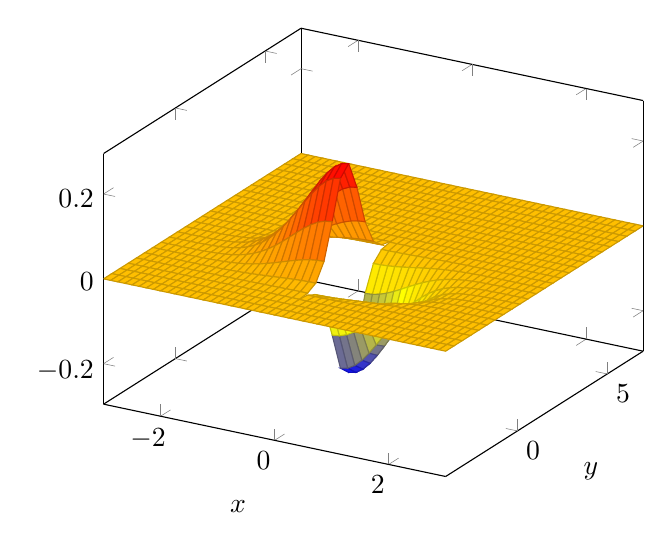
\begin{tikzpicture}
					\begin{axis}[
						view={30}{30},
						xlabel=$x$, ylabel=$y$
					]
					\addplot3[surf, domain =3:0, domain y=-4:7] {-1/4*exp(-x^2-y^2)};
					\addplot3[surf, domain =-3:0, domain y=-4:7] {1/4*exp(-x^2-y^2)};
					\end{axis}
				\end{tikzpicture}
			}
		\end{subfigure}
		\begin{subfigure}{.49\textwidth}
			\centering
			\resizebox{\linewidth}{!}{
				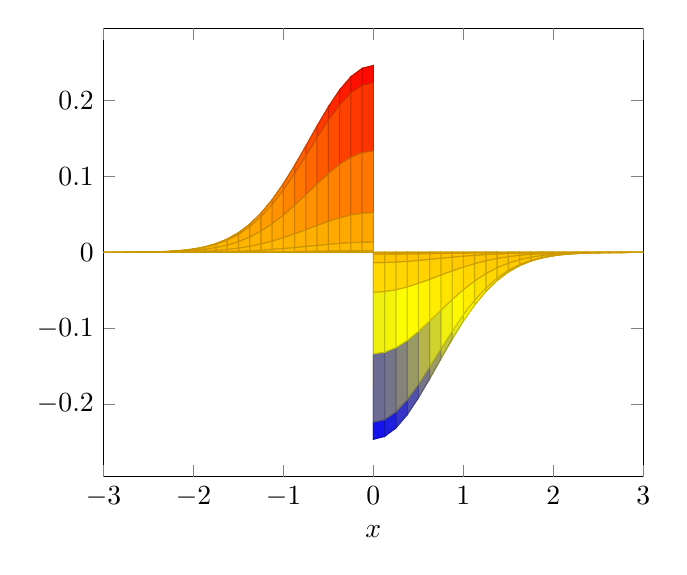
\begin{tikzpicture}
					\begin{axis}[
						view={0}{0},
						xlabel=$x$, ylabel=$y$
					]
					\addplot3[surf, domain =3:0, domain y=-4:7] {-1/4*exp(-x^2-y^2)};
					\addplot3[surf, domain =-3:0, domain y=-4:7] {1/4*exp(-x^2-y^2)};
					\end{axis}
				\end{tikzpicture}
			}
		\end{subfigure}
	\end{figure}
\end{example}
\begin{exercise}
	Sia $f:\R^2 \to \R^m$ derivabile in $x_0$, con $x_0 \in \R^2$. Sia $g:\R^2 \to \R^m$ definita da $g(x,y) = f(y,x)$\\
	Come sono legate le derivate parziali di $f$ e $g$ in $x_0$?
	% TODO solution
\end{exercise}
\begin{exercise}
	Sia $f:A \to \R$ con $A \subseteq \R^n$, derivabile in $x_0 \in \circdot{A}$ . Determinare le derivate parziali in $x_0$ delle funzioni
	\begin{itemize}
		\item $F:A \to \R^2$ definita da $\bigl( f(x), f(x) \bigr)$
		\item $G:A \times A \to \R$ definita da $G(x,y) = f(x) + f(y)$
	\end{itemize}
	% TODO solution
\end{exercise}
\begin{proposition}
	Siano $A \subseteq \R^n$ e $x_0 \in \circdot{A}$. $f$ è \textbf{derivabile parzialmente} rispetto alla $i$-esima coordinata se e solo \textbf{se esiste} finito il limite
	\begin{equation}
		\label{eq:deriv_i_esima}
		\lim\limits_{t \to 0} \frac{f(x_1,\:\dotsc\:,x_i+t,\:\dotsc\:,x_n) - f(x_1,\:\dotsc\:,x_i,\:\dotsc\:,x_n)}{t}
	\end{equation}
	\begin{proof}
		Da \fullref{def:deriv_direz}, sceglendo $v = e_i$ della base canonica si ottiene la \cref{eq:deriv_i_esima}
	\end{proof}
\end{proposition}
\begin{exercise}
	\label{ex:funz_derivabili}
	Formulare in modo rigoroso e dimostrare:
	\begin{enumerate}
		\item La somma di funzioni parzialmente derivabili è parzialmente derivabile.
		\item La composizione di funzioni parzialmente derivabili è parzialmente derivabile.
		\item Prodotto e rapporto, quando definiti, di funzioni parzialmente derivabili sono funzioni parzialmente derivabili.
	\end{enumerate}
	% TODO solution
\end{exercise}
\begin{example}
	Sia $f: \R^2 \to \R^3$ data da
	\begin{equation*}
		f(x,y) =
		\begin{bmatrix}
			2x + 3y\\
			\sin (xy^2)\\
			e^{xy}
		\end{bmatrix}
	\end{equation*}
	La funzione $f$ è derivabile parzialmente su tutto $\R^2$. Inoltre
	\[
		\frac{\partial f}{\partial x}(x,y) =
		\begin{bmatrix}
			2\\
			y^2 \cos (xy^2)\\
			y e^{xy}
		\end{bmatrix}
		\qquad\qquad
		\frac{\partial f}{\partial y}(x,y) =
		\begin{bmatrix}
			3\\
			2xy \cos (xy^2)\\
			x e^{xy}
		\end{bmatrix}
	\]
\end{example}

\begin{proposition}
	Siano $A \subseteq \R^n$, $x_0 \in \circdot{A}$ e $v \in \R^n$ con $v \neq 0$. Sia $f: A \to \R^m$, allora
	\begin{equation*}
		\begin{gathered}
			f \text{ è \textbf{Derivabile} in $x_0$ nella direzione $v$}\\
			\iff\\
			\forall i = 1,\:\dotsc\:,m \quad \text{la \textbf{componente} $f_i$ \textbf{è derivabile} in $x_0$ nella direzione $v$}
		\end{gathered}
	\end{equation*}
	\begin{proof}
		Applicando \fullref{prop:succ_conv_se_comp_conv} e \fullref{prop:cont_e_cont_per_succ} % TODO proper proof. This does not make sense as of now, I know.
	\end{proof}
\end{proposition}
\begin{exercise}
	\label{ex:deriv_non_impl_cont}
	La derivabilità in ogni direzione non implica la continuità. Verificare che la funzione
	\[\funcdef{f}{\R^2}{\R}{(x,y)}
	{
		\begin{cases}
			1 \qquad \text{se } y = x^2 \text{ e } x \neq 0\\
			0 \qquad \text{altrimenti}
		\end{cases}
	}\]
	ammette nell'origine derivate direzionali in ogni direzione ma che \textit{non} è continua nell'origine.
	\begin{figure}[H]
		\begin{subfigure}{.49\textwidth}
			\centering
			\resizebox{\linewidth}{!}{
				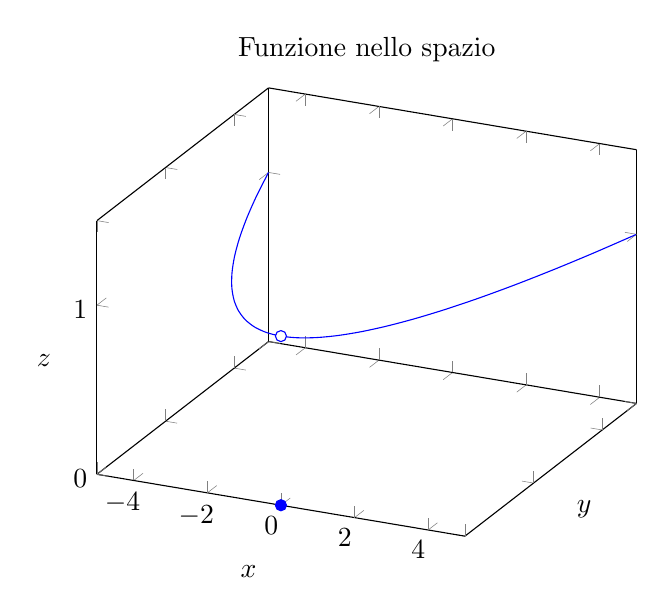
\begin{tikzpicture}
					\begin{axis}[
						title={Funzione nello spazio},
						xlabel=$x$, ylabel=$y$, zlabel=$z$, zlabel style={rotate=-90},
						yticklabels={,,},
						samples y=0,
						zmin = 0, zmax = 1.5
					]
					\addplot3 [smooth, color=blue] (x,x^2,1);
					\addplot3 [color=blue, fill=white, only marks,mark=*] coordinates{(0,0,1)};
					\addplot3 [color=blue, only marks, mark=*] coordinates{(0,0,0)};
					\end{axis}
				\end{tikzpicture}
			}
		\end{subfigure}
		\begin{subfigure}{.49\textwidth}
			\centering
			\resizebox{\linewidth}{!}{
				\begin{tikzpicture}
					\node at (3.4, .2) {$0$};

					\node at (2.1, 1.1) {$1$};
					\node at (4.8, 1.1) {$1$};
					\node at (1.2, 2.5) {$1$};
					\node at (5.65, 2.5) {$1$};
					\node at (.4, 4.5) {$1$};
					\node at (6.5, 4.5) {$1$};

					\node at (1.7, .2) {$0$};
					\node at (6, .6) {$0$};
					\node at (2.6, 2.2) {$0$};
					\node at (5, 3) {$0$};
					\node at (3.2, 4.3) {$0$};
					\node at (1.8, 5) {$0$};
					\begin{axis} [
						title={Valori della $z$},
						axis lines = center,
						xlabel=$x$, ylabel=$y$,
						xticklabels={,,}, yticklabels={,,},
						ymin = -1
					]
						\addplot[color=blue!70, smooth] {x^2};
					\end{axis}
				\end{tikzpicture}
			}
		\end{subfigure}
	\end{figure}

	\begin{solution}
		Le derivate direzionali sono
		\begin{align*}
			\partial_x f(0,0) &= \lim\limits_{t \to 0} \frac{f(0+t,0)-f(0,0)}{t} = 0\\
			\partial_y f(0,0) &= \lim\limits_{t \to 0} \frac{f(0,0+t)-f(0,0)}{t} = 0\\
			D_v f(0,0) &= \lim\limits_{t \to 0} \frac{f(0+t_1,0+t_2)-f(0,0)}{t} = 0
		\end{align*}
		Dunque, per ogni derivata parziale o direzionale in $(0,0)$ il valore della derivata sarà $0$.\\
		D'altro canto $f$ in $0$ \textit{non} è continua in $(0,0)$, quindi si è verificato che la derivabilità non implichi la continuità con $\dim A > 1$
	\end{solution}
\end{exercise}
\begin{exercise}
	Esibire una funzione $f: \R^2 \to \R$ che ammetta in (almeno) un punto una derivata parziale rispetto ad $x$ ma non rispetto a $y$
	\begin{solution}
		La
		\[\funcdef{f}{\R^2}{\R}{(x,y)}{x+\sqrt{y}}\]
		È derivabile parzialmente rispetto a $x$ ma non rispetto a $y$ in $(0,0)$, infatti
		\begin{align*}
			\partial_x f(0,0) &= \lim\limits_{t \to 0} \frac{f(0+t,0)-f(0,0)}{t} = \frac{t-0}{t} = 1\\
			\partial_y f(0,0) &= \lim\limits_{t \to 0} \frac{f(0,0+t)-f(0,0)}{t} = \frac{\sqrt{t}-0}{t} = +\infty \implies \nexists \text{ limite finto}
		\end{align*}
	\end{solution}
\end{exercise}

\newpage
\section{Derivata Totale}
\begin{theorem}[di Lagrange]\leavevmode\vspace*{-\baselineskip}
	\label{teo:lagrange}
	\begin{note}
		Questo teorema viene trattato approfonditamente nel corso di Analisi 1 e si applica solo a funzioni $\R^1 \to \R^1$, qui verrà solo riportato rapidamente l'enunciato
	\end{note}
	\begin{note}
		Questo teorema è anche noto come \textit{Teorema del Valor Medio Differenziale}
	\end{note}
	Sia $f: \intervalclose{a}{b} \to \R$ una funzione \textbf{Continua} nell'intervallo chiuso $\intervalclose{a}{b}$ e \textbf{Derivabile} nell'intervallo aperto $\intervalopen{a}{b}$. Allora esiste almeno un punto
	\[c \in \intervalopen{a}{b} : f'(c) = \frac{f(b)-f(a)}{b - a}\]
	O, alternativamente, nella forma
	\[\xi \in \intervalopen{0}{1} : f'(x_0 + \xi h) = \frac{f(x_0 + h)-f(x_0)}{h}\]
\end{theorem}
\begin{definition}[o piccolo]
	\label{def:o_piccolo}
	Siano $A \subseteq \R^n$ e $x_0 \in \circdot{A}$. Siano $f,g: A \to \R^m$ due funzioni.
	\[f=o(g) \text{ per } x \to x_0 \qquad \bydef \qquad \lim\limits_{x \to x_0} \frac{\norm{f(x)}}{\norm{g(x)}} = 0\]
	che si legge $f$ è \textbf{o piccolo} di $g$.
	\begin{note}
		Scrivere $f(x) = o(x^k)$ per $x \to 0$ significa che $f = o(g)$ con $g = x^k$
	\end{note}
	\begin{note}
		Con $o(1)$ per $x \to x_0$ si intende una qualunque funzione tendente a $0$ per $x \to x_0$.
	\end{note}
\end{definition}
\begin{exercise}
	Perché son state utilizzate le norme nella \fullref{def:o_piccolo}?
	\begin{solution}
		Perché l'operazione di divisione è sensata solo tra due scalari, non tra vettori.
	\end{solution}
\end{exercise}
\begin{exercise}
	Quali tra le seguenti uguaglianze sono vere? (In tutte, $x \to 0$)
	\begin{itemize}
		\begin{minipage}{0.33\linewidth}
			\item $o(x) = o(x) + o(x)$
			\item $o(x^2) = o(x) \cdot o(x)$
			\item $o(x^2) = o(x) - o(x)$
		\end{minipage}
		\begin{minipage}{0.33\linewidth}
			\item $\sqrt{x} = o(x)$
			\item $o(x) = \abs{o(x)}$
			\item $x = o(\sqrt{x})$
		\end{minipage}
		\begin{minipage}{0.33\linewidth}
			\item $o(x) = 10^6 o(x)$
			\item $x + x^2 = o(x)$
			\item $x = o(x + x^2)$
		\end{minipage}
	\end{itemize}
\end{exercise}
\vspace*{\baselineskip}
La seguente definizione è da ritenersi già nota da Analisi 1
\begin{definition}[Derivata in $\R$]
	Siano $A \subseteq \R$ e $x_0 \in \circdot{A}$. Sia $f: A \to \R$
	\[f \text{ \textbf{Derivabile} in } x_0 \quad \bydef \quad \lim\limits_{h \to 0} \frac{f(x_0 + h) - f(x_0)}{h} \text{  esiste finito}\]
\end{definition}

Direttamente dalla nozione di Analisi 1 di derivata, si ottiene la seguente relazione tra derivata e coefficiente angolare della retta tangente in un punto
\begin{proposition}[Derivata Analisi 1]
	\label{prop:deriv_analisi_1}
	Siano $A \subseteq \R$ e $x_0 \in \circdot{A}$. Sia $f: A \to \R$
	\begin{equation*}
		\begin{gathered}
			f \text{ è derivabile in } x_0\\
			\iff\\
			\exists m \in \R:\; f(x_0+h) = f(x_0) + mh +o(h) \text{ per } h \to 0
		\end{gathered}
	\end{equation*}
	\begin{proof}
		\begin{align*}
			& f \text{ è derivabile in } x_0\\
			\iff & \lim\limits_{h \to 0} \frac{f(x_0 + h) - f(x_0)}{h} \text{  esiste finito}\\
			\iff & \exists m \in \R:\; \lim\limits_{h \to 0} \frac{f(x_0 + h) - f(x_0)}{h} = m\\
			\iff & \exists m \in \R:\; \lim\limits_{h \to 0} \frac{f(x_0 + h) - f(x_0)}{h} - m = 0\\
			\iff & \exists m \in \R:\; \lim\limits_{h \to 0} \frac{f(x_0 + h) - f(x_0) -mh}{h} = 0
			\shortintertext{Per la nota alla \fullref{def:o_piccolo}}
			\iff & \exists m \in \R:\; f(x_0 + h) - f(x_0) -mh = o(h) \text{ per } h \to 0\\
			\iff & \exists m \in \R:\; f(x_0 + h) = f(x_0) -mh + o(h) \text{ per } h \to 0
		\end{align*}
	\end{proof}
\end{proposition}

\noindent Analogamente a quanto fatto nella \fullref{prop:deriv_analisi_1}, si definisce
\begin{definition}[Differenziale]
	\label{def:differenz}
	Siano $A \subseteq \R^n$ e $x_0 \in \circdot{A}$. Sia $f: A \to \R^m$
	\begin{equation*}
		\begin{gathered}
			f \text{ è \textbf{Differenziabile} in } x_0\\
			\bydef\\
			\exists M \in \mat (m \times n):\; f(x_0 + h) = f(x_0) + Mh + o(h) \text{ per } h \to 0
		\end{gathered}
	\end{equation*}
	La matrice $M$ è la \textbf{Derivata Totale} di $f$ calcolata in $x_0$ e si indica con $Df(x_0)$. $Df(x_0)$ è l'applicazione \textit{lineare} che meglio approssima la variazione di $f$ nelle vicinanze di $x_0$.
	\begin{note}
		Verrà spiegato più avanti in \fullref{coro:se_diff_deriv_parz} un metodo pratico di calcolo della Derivata Totale.
	\end{note}
\end{definition}
\begin{observation}[Matrici Derivata Totale Particolari]
	\label{obs:matr_deriv_tot}
	Data la matrice $Df(x_0)$ con $m$ righe e $n$ colonne:
	\begin{itemize}
		\item Se $n = 1$ e $m = 1$ $Df(x_0)$ è \textbf{Derivata} di Analisi 1, uno scalare
		\item Se $n > 1$ e $m = 1$ $Df(x_0)$ è \textbf{Gradiente} di $f$ e si indica con $\nabla f(x_0)$ (\textit{nabla} $f$) o $\grad f(x_0)$
		\item Se $n = 1$ e $m > 1$ $Df(x_0)$ è \textbf{Vettore Tangente} alla $f$
		\item Se $n > 1$ e $m > 1$ $Df(x_0)$ è \textbf{Matrice Jacobiana} di $f$ e si può anche indicare con $J_f(x_0)$
	\end{itemize}
	Come si vedrà in \fullref{coro:se_diff_deriv_parz}, il Gradiente della \textit{i-esima} variabile è la \textit{i-esima} colonna di $Df(x_0)$.\\
	Il Vettore Tangente della \textit{j-esima} variabile è invece la \textit{j-esima} riga di $Df(x_0)$.
\end{observation}
\begin{example}
	Esempi relazioni tra Derivata Totale e derivate parziali
	\begin{align*}
		n = 2 \quad m = 1 \qquad & Df =
		\begin{bmatrix}
			\frac{\partial f}{\partial x} & \frac{\partial f}{\partial y}
		\end{bmatrix}\\
		n = 3 \quad m = 1 \qquad & Df =
		\begin{bmatrix}
			\frac{\partial f}{\partial x} & \frac{\partial f}{\partial y} &  \frac{\partial f}{\partial z}
		\end{bmatrix}\\
		n = 1 \quad m = 2 \qquad & Df =
		\begin{bmatrix}
			\frac{\partial f_1}{\partial x}\\[1ex]
			\frac{\partial f_2}{\partial x}
		\end{bmatrix}\\
		n = 2 \quad m = 2 \qquad & Df =
		\begin{bmatrix}
			\frac{\partial f_1}{\partial x} & \frac{\partial f_1}{\partial y}\\[1ex]
			\frac{\partial f_2}{\partial x} & \frac{\partial f_2}{\partial y}
		\end{bmatrix}\\
		n > 2 \quad m > 2 \qquad & Df =
		\begin{bmatrix}
			\frac{\partial f_1}{\partial x_1} & \frac{\partial f_1}{\partial x_2} & \dots & \frac{\partial f_1}{\partial x_n}\\[1ex]
			\frac{\partial f_2}{\partial x_1} & \frac{\partial f_2}{\partial x_2} & \dots & \frac{\partial f_2}{\partial x_n}\\[1ex]
			\vdots & \vdots & \ddots & \vdots\\[1ex]
			\frac{\partial f_m}{\partial x_1} & \frac{\partial f_m}{\partial x_2} & \dots & \frac{\partial f_m}{\partial x_n}
		\end{bmatrix}\\
	\end{align*}
\end{example}
\begin{exercise}
	Perché non è stata data una definizione di derivata attraverso il limite del rapporto incrementale?
	% TODO solution
\end{exercise}
\begin{example}
	Siano $M \in \mat(m \times n)$ una matrice fissata, $f: \R^n \to \R^m$ data da $f(x) = Mx$.\\
	Allora $f$ è differenziabile ovunqe e per ogni $x_0 \in \R$ si ha $Df(x_0) = M$
\end{example}
\begin{proposition}[Unicità della Derivata Totale]
	\label{prop:unic_deriv_tot}
	Siano $A \subseteq \R^n$, $x_0 \in \circdot{A}$, $f: A \to \R^m$ e $M_1, M_2 \in \mat(m \times n)$
	\begin{equation*}
		\left.
		\begin{array}{l}
			M_1 \text{ derivata totale di } f \text{ in } x_0\\
			M_2 \text{ derivata totale di } f \text{ in } x_0
		\end{array}
		\right\}
		\implies
		M_1 = M_2
	\end{equation*}
	\begin{proof}
		Sia $h \in \R$. Fissato un vettore $e_i$ della base canonica di $\R^n$
		\begin{align*}
			M_2 e_i - M_1 e_1 &=\\
			\shortintertext{Moltiplicando e dividendo per $h$}
			&= \frac{1}{h} M_2 e_i h - \frac{1}{h} M_1 e_i h\\
			&= \frac{1}{h} [M_2 e_i h - M_1 e_i h]
			\shortintertext{Grazie alla \fullref{def:differenz}}
			&= \frac{1}{h} [f(x_0 + h e_i) - f(x_0) + o(h)] - \frac{1}{h} [f(x_0 + h e_i) - f(x_0) + o(h)]\\
			&= o(h) \text{ per } t \to 0
		\end{align*}
		Passando al limite per $t \to 0$, si deduce che le applicazioni lineari $M_1$ e $M_2$ hanno le stesse immagini sui vettori della base canonica, quindi coincidono.
	\end{proof}
\end{proposition}
\begin{proposition}
	Siano $A \subseteq \R^n$, $x_0 \in \circdot{A}$ e $f:A \to \R^m$
	\[f \text{ \textbf{Differenziabile} in } x_0 \implies f \text{ \textbf{Continua} in } x_0\]
	\begin{proof}
		Per ipotesi $x_0 \in \circdot{A}$, dunque $x_0$ è di accumulazione. A questo punto, grazie alla \fullref{prop:f_cont_se_isol_o_accum} basta verificare che $\lim\limits_{x \to x_0} f(x) = f(x_0)$.
		Dalla \fullref{def:differenz}
		\[f(x_0 + h) = f(x_0) + Mh + o(h) \text{ per } h \to 0\]
		Quindi, posto $h = x - x_0$ ed essendo $M = Df(x_0)$ per \fullref{def:differenz}
		\[\lim\limits_{x \to x_0} f(x) = \lim\limits_{x \to x_0} \bigl[f(x_0) + Df(x_0)(x-x_0) + o(x - x_0)\bigr] = f(x_0)\]
	\end{proof}
\end{proposition}
\begin{proposition}
	\label{prop:se_diff_deriv_dir}
	Siano $A \subseteq \R^n$, $x_0 \in \circdot{A}$ e $f:A \to \R^m$
	\[
		f \text{ \textbf{Differenziabile} in } x_0
		\implies
		\begin{cases}
			\begin{array}{c}
				f \text{ ammette ogni \textbf{Derivata Direzionale} in } x_0\\[-1ex]
				e\\[-1ex]
				\forall v \in \R^n \setminus \brackets{0} D_v f(x_0) = Df(x_0)v
			\end{array}
		\end{cases}
	\]
	\begin{proof}
		Sia $v \in \R^n$ non nullo. Partendo dalla \fullref{def:deriv_direz}
		\begin{align*}
			&\lim\limits_{t \to 0} \frac{f(x_0 + tv) - f(x_0)}{t}
			\shortintertext{Sostituendo ora $f(x_0 + tv)$ con il secondo membro della \fullref{def:differenz}, dopo aver posto $h = tv$}
			= &\lim\limits_{t \to 0} \frac{\cancel{f(x_0)} + Df(x_0)(tv) + o(tv) - \cancel{f(x_0)}}{t}\\
			= &\lim\limits_{t \to 0} \frac{Df(x_0)(tv)}{t} + \lim\limits_{t \to 0} \frac{o(tv)}{t}\\
			= &Df(x_0)v
		\end{align*}
	\end{proof}
\end{proposition}
\begin{corollary}
	\label{coro:se_diff_deriv_parz}
	Siano $A \subseteq \R^n$, $x_0 \in \circdot{A}$ e $f:A \to \R^m$
	\[
		f \text{ \textbf{Differenziabile} in } x_0
		\implies
		\begin{cases}
			\begin{array}{c}
				f \text{ ammette ogni \textbf{Derivata Parziale} in } x_0\\
				e\\
				\frac{\partial f}{\partial x_i}(x_0) = Df(x_0) \cdot e_i
			\end{array}
		\end{cases}
	\]
	Dove $Df(x_0) \cdot e_i$ non è altro che
	\[
		Df(x_0) \cdot e_i =
		\begin{bmatrix}
			x_{11} & \cdots & x_{1i} & \cdots & x_{1n}\\
			x_{21} & \cdots & x_{2i} & \cdots & x_{2n}\\
			\vdots & \vdots & \vdots & \ddots & \vdots\\
			x_{n1} & \cdots & x_{ni} & \cdots & x_{nn}\\
		\end{bmatrix}
		\cdot
		\begin{bmatrix}
			(0 & \dots & 1 & \dots & 0)
		\end{bmatrix}
		=
		\begin{bmatrix}
			0 & \cdots & x_{1i} & \cdots & 0\\
			0 & \cdots & x_{2i} & \cdots & 0\\
			\vdots & \vdots & \vdots & \ddots & \vdots\\
			0 & \cdots & x_{ni} & \cdots & 0\\
		\end{bmatrix}
	\]
	Cioè l'\textit{i-esima} colonna della $Df(x_0)$, come da \fullref{obs:matr_deriv_tot}
	\begin{note}
		Per quanto detto, il presente corollario offre il principale metodo di calcolo della \textbf{Derivata Totale}\\
		Inoltre è anche una dimostrazione alternativa della \fullref{prop:unic_deriv_tot}
	\end{note}
	\begin{proof}
		Direttamente dalla \fullref{prop:se_diff_deriv_dir} e dalla \fullref{def:deriv_direz} (sezione sulle derivate parziali)
	\end{proof}
\end{corollary}
\begin{observation}
	Sia \fullref{prop:se_diff_deriv_dir} che \fullref{coro:se_diff_deriv_parz} non possono essere invertiti, come verificato in \fullref{ex:deriv_non_impl_cont}.
\end{observation}
\begin{corollary}
	Siano $A \subseteq \R^n$, $x_0 \in \circdot{A}$ e $f:A \to \R^m$
	\[f \text{ \textbf{Differenziabile} in } x_0 \implies f \text{ \textbf{Derivabile} in } x_0\]
	\begin{proof}
		Mediante il \fullref{coro:se_diff_deriv_parz} si vede immediatamente che rispetta la \fullref{def:deriv_direz}
	\end{proof}
\end{corollary}
\begin{corollary}
	\label{coro:f_diff_con_matr_comp}
	Siano $A \subseteq \R^n$, $x_0 \in \circdot{A}$ e $f:A \to \R^m$. Sia $f$ derivabile parzialmente in $x_0$ e sia $M$ la $Df(x_0)$, matrice dei coefficienti $M_{ij} = \frac{\partial f_i}{\partial x_j}$
	\begin{equation*}
		\begin{gathered}
			f \text{ \textbf{Differenziabile} in } x_0\\
			\iff\\
			f(x_0 + h) - f(x_0) - Mh = o(h) \text{ per } h \to 0
		\end{gathered}
	\end{equation*}
	\begin{proof}
		Direttamente dalla \fullref{def:differenz}, per mezzo del \fullref{coro:se_diff_deriv_parz}.
	\end{proof}
\end{corollary}
\begin{exercise}
	Verificare che, nel caso $n = 2$ ed $m = 1$ il \fullref{coro:f_diff_con_matr_comp} si scrive
	\begin{equation*}
		\begin{gathered}
			f \text{ \textbf{Differenziabile} in } x_0\\
			\iff\\
			f(x_0 + h, y_o + k) - f(x_0, y_0) -
			\begin{bmatrix}
				\frac{\partial f}{\partial x}(x_0, y_0) & \frac{\partial f}{\partial y}(x_0, y_0)
			\end{bmatrix}
			\cdot
			\begin{bmatrix}
				h\\
				k
			\end{bmatrix}
			= o(\sqrt{h^2 + k^2}) \text{ per } h, k \to 0
		\end{gathered}
	\end{equation*}
	% TODO solution
\end{exercise}
\begin{exercise}
	Scrivere il \fullref{coro:f_diff_con_matr_comp} nel caso $n = 3$ ed $m = 1$
	% TODO solution
\end{exercise}

\begin{theorem}[del Differenziale Totale]
	\label{teo:diff_tot}
	Siano $A \subseteq \R^n$, $x_0 \in \circdot{A}$ e $f:A \to \R^m$.
	\[
		\left.
		\text{
			\begin{tabular}{c}
				Per $i = 1,\:\dotsc\:,m$ e $j = 1,\:\dotsc\:,n$\\
				$\frac{\partial f_i}{\partial x_j}$ è \textbf{definita} in un \textbf{intorno} di $x_0$ e \textbf{Continua} in $x_0$
			\end{tabular}
		}
		\right\}
		\implies\\
		f \text{ è \textbf{Differenziabile} in } x_0
	\]
	\vspace*{-\baselineskip}
	\begin{note}
		È specificata la necessità di continuità in un intorno di $x_0$ in quanto, come detto in \fullref{def:deriv_direz}, l'esistenza di derivate parziali non garantisce la continuità.
	\end{note}
	\begin{proof}
		Si può supporre $n = 2$ e $m = 1$ in quanto il caso più generale è del tutto analogo.\\
		È necessario verificare la \fullref{def:differenz}, dunque in $\R^n = \R^2$ si ha
		\begin{equation}
			\label{eq:deriv_tot_def_diff}
			f(x_0 + h, y_0 + k) = f(x_0, y_0) + Df(x_0, y_0) \begin{bmatrix}h\\k\end{bmatrix} + o(h,k) \text{ per } h,k \to 0
		\end{equation}
		Considerando solo i primi due addendi, aggiungendo e sottraendo la stessa quantità, si ottiene
		\begin{equation}
			\label{eq:teo_diff_tot_sommo_sottraggo}
			f(x_0 + h, y_0 + k) - f(x_0, y_0) = \underbrace{f(x_0 + h, y_0 + k) - f(x_0+h,y_0)}_{\text{(1)}} + \underbrace{f(x_0+h,y_0) - f(x_0, y_0)}_{\text{(2)}}
		\end{equation}
		Considerando la (1) e la (2) di \cref{eq:teo_diff_tot_sommo_sottraggo} come funzioni in una sola variabile, si può applicare il \fullref{teo:lagrange}
		\begin{itemize}
			\item La (1) rispetto a $y$, con $x_0 + h$ fissato
			\item La (2) rispetto a $x$, con $y_0$ fissato
		\end{itemize}
		Spostandosi lungo le direzioni parallele agli assi è possibile andare da $(x_0 + h, y_0 + k)$ a $(x_0, y_0)$
		\begin{center}
			\begin{tikzpicture}
				\pgfmathsetmacro\MAX{8}
				\pgfmathsetmacro\XZ{\MAX / 3 }
				\pgfmathsetmacro\YZ{\MAX / 3 }
				\pgfmathsetmacro\XZh{\MAX / 3 *2}
				\pgfmathsetmacro\YZk{\MAX / 3 *2}
				\coordinate (X0Y0) at (\XZ,\YZ);
				\coordinate (X0hY0) at (\XZh,\YZ);
				\coordinate (X0Y0k) at (\XZ,\YZk);
				\coordinate (X0hY0k) at (\XZh,\YZk);

				\draw[->] (0,0) -- (\MAX,0) node[anchor=north west] {$x$};
				\draw[->] (0,0) -- (0,\MAX) node[anchor=south east] {$y$};
				\draw[dotted] (\XZ,0) -- (\XZ,\MAX);
				\draw[dotted] (0,\YZ) -- (\MAX,\YZ);
				\draw[dotted] (\XZh,0) -- (\XZh,\MAX);
				\draw[dotted] (0,\YZk) -- (\MAX,\YZk);
				\draw node[anchor=north] at (\XZ,0) {$x_0$};
				\draw node[anchor=north] at (\XZh,0) {$x_0+h$};
				\draw node[anchor=east] at (0,\YZ) {$y_0$};
				\draw node[anchor=east] at (0,\YZk) {$y_0+k$};
				\draw node at (X0Y0) {$\bullet$};
				\draw node at (X0Y0k) {$\bullet$};
				\draw node at (X0hY0) {$\bullet$};
				\draw node at (X0hY0k) {$\bullet$};
				\draw node[anchor=north east] at (X0Y0) {$(x_0,y_0)$};
				\draw node[anchor=south east] at (X0Y0k) {$(x_0,y_0+k)$};
				\draw node[anchor=north west] at (X0hY0) {$(x_0+h,y_0)$};
				\draw node[anchor=south west] at (X0hY0k) {$(x_0+h,y_0+k)$};

				\draw[<-] (\XZ,\MAX*4/10) -- (\XZ,\MAX*6/10);
				\draw[<-] (\XZh,\MAX*4/10) -- (\XZh,\MAX*6/10);
				\draw[<-] (\MAX*4/10,\YZ) -- (\MAX*6/10,\YZ);
				\draw[<-] (\MAX*4/10,\YZk) -- (\MAX*6/10,\YZk);
			\end{tikzpicture}
		\end{center}
		Quindi, applicando il \fullref{teo:lagrange}:
		\[
			\exists \alpha, \beta \in \intervalopen{0}{1} \textbf{ per cui} \qquad
			\begin{array}{rrcl}
				\text{(1)} & f(x_0 + h, y_0 + k) - f(x_0 + h, y_0) &=& \frac{\partial f}{\partial y} (x_0 + h, y_0 + \beta k) k\\[1ex]
				\text{(2)} & f(x_0 + h, y_0) - f(x_0, y_0) &=& \frac{\partial f}{\partial x} (x_0 + \alpha h, y_0) h
			\end{array}
		\]
		Tornando alla \cref{eq:deriv_tot_def_diff}, si ottiene
		\begin{align*}
			&f(x_0 + h, y_0 + k) - f(x_0, y_0) - Df(x_0, y_0) \begin{bmatrix}h\\k\end{bmatrix}\\
			= &\underbrace{f(x_0 + h, y_0 + k) - f(x_0+h,y_0)}_{\text{(1)}} + \underbrace{f(x_0+h,y_0) - f(x_0, y_0)}_{\text{(2)}} - Df(x_0, y_0) \begin{bmatrix}h\\k\end{bmatrix}\\
			= &\underbrace{\frac{\partial f}{\partial y} (x_0 + h, y_0 + \beta k) k}_{\text{(1)}} + \underbrace{\frac{\partial f}{\partial x} (x_0 + \alpha h, y_0) h}_{\text{(2)}} - Df(x_0, y_0) \begin{bmatrix}h\\k\end{bmatrix}
			\shortintertext{Si esegue il prodotto tra matrice Derivata Totale e vettore, infine si separano i termini}
			= &	\left( \frac{\partial f}{\partial y} (x_0 + h, y_0 + \beta k) - \frac{\partial f}{\partial y} (x_0 + h, y_0) \right) k +
				\left( \frac{\partial f}{\partial x} (x_0 + \alpha h, y_0) - \frac{\partial f}{\partial x} (x_0, y_0)\right) h
		\end{align*}
		Si passa dunque alla norma
		\begin{align*}
			&\norm{f(x_0 + h, y_0 + k) - f(x_0, y_0) - Df(x_0, y_0) \begin{bmatrix}h\\k\end{bmatrix}}\\
			\shortintertext{Separando come fatto prima ed applicando la disguguaglianza triangolare}
			\leq &	\norm{\left( \frac{\partial f}{\partial y} (x_0 + h, y_0 + \beta k) - \frac{\partial f}{\partial y} (x_0 + h, y_0) \right) k} +
					\norm{\left( \frac{\partial f}{\partial x} (x_0 + \alpha h, y_0) - \frac{\partial f}{\partial x} (x_0, y_0)\right) h}
			\shortintertext{Per proprietà 4 da \fullref{def:norma}}
			= & \norm{\frac{\partial f}{\partial y} (x_0 + h, y_0 + \beta k) - \frac{\partial f}{\partial y} (x_0 + h, y_0)} \abs{k} +
				\norm{\frac{\partial f}{\partial x} (x_0 + \alpha h, y_0) - \frac{\partial f}{\partial x} (x_0, y_0)} \abs{h}
			\shortintertext{Presa ora la norma del vettore $(h,k)$, cioè $\norm{(h,k)} = \sqrt{h^2 + k^2}$, sicuramente $\abs{h} \leq \norm{(h,k)}$ e $\abs{k} \leq \norm{(h,k)}$, dunque}
			\leq &	\norm{\frac{\partial f}{\partial y} (x_0 + h, y_0 + \beta k) - \frac{\partial f}{\partial y} (x_0 + h, y_0)} \sqrt{h^2 + k^2} +
					\norm{\frac{\partial f}{\partial x} (x_0 + \alpha h, y_0) - \frac{\partial f}{\partial x} (x_0, y_0)} \sqrt{h^2 + k^2}
			\shortintertext{Essendo $h,k \to 0$ da \cref{eq:deriv_tot_def_diff} e graze alla continuità delle derivate, le due norme tendono a $0$. Inoltre, per \fullref{def:o_piccolo}}
			=\; &o(1) \sqrt{h^2 + k^2} \text{ per } \begin{bmatrix}h\\k\end{bmatrix} \to 0\\
			=\; &o(\sqrt{h^2 + k^2}) \text{ per } \begin{bmatrix}h\\k\end{bmatrix} \to 0
		\end{align*}
		Da cui la tesi, avendo verificato la \fullref{def:differenz}.
	\end{proof}
\end{theorem}
\begin{exercise}
	Data la funzione
	\[
		\funcdef{f}{\R}{\R}{x}{
			\begin{cases}
				\begin{array}{ll}
					x^2 \sin \frac{1}{x} & x \neq 0\\
					0 & x = 0
				\end{array}
			\end{cases}
		}
	\]
	Verificare che $f$ è differenziabile su $\R$ ma non ha derivata continua su $\R$.
	% TODO solution
\end{exercise}

\begin{definition}[Funzioni di Classe $\cntclass{1}$]
	Sia $A \subseteq \R^n$ un \textbf{Aperto}.
	\begin{center}
		$\cntclass{1}(A; \R^m)$ è l'insieme delle funzioni $f:A \to \R^m$\\
		con \textbf{tutte} le \textbf{Derivate Parziali prime continue} in ogni punto di $A$
	\end{center}
	Si può anche leggere \textit{$f$ è di classe $\cntclass{1}$ su $A$ con valori in $\R^m$}.
\end{definition}
\begin{corollary}
	Sia $A \subseteq \R^n$ un \textbf{Aperto}. Se $f \in \cntclass{1}(A;\R^m)$ allora $f$ è \textbf{Differenziabile} su $A$.
	\begin{proof}
		Applicare la \fullref{teo:diff_tot}
	\end{proof}
\end{corollary}
\begin{proposition}
	\label{prop:cnt_class_components}
	Siano $m \in \N, m \geq 1$ e $A \subseteq \R^n$ un \textbf{Aperto}
	\[f \in \cntclass{1}(A; \R^m) \iff \forall i = 1,\:\dotsc\:, m \quad f_i \in \cntclass{1}(A;\R)\]
	\begin{proof}
		Immediata.
	\end{proof}
\end{proposition}
\begin{exercise}
	Dimostrare la \fullref{prop:cnt_class_components}.
	% TODO solution
\end{exercise}
\begin{exercise}
	Dimostrare che $\cntclass{1}(A;\R)$ non coincide con l'insieme delle funzioni differenziabili su $A$ con valori in $\R$.
	% TODO solution
\end{exercise}
\begin{proposition}
	\label{prop:if_df_lim_then_unif_cont}
	Siano $I \in \R$ un intervallo reale e $f(x)$ una funzione \textbf{Derivabile} in $I$. Se la $f'(x)$ è una \textbf{Funzione Limitata} in $I$, allora f è \textbf{Uniformemente Continua} in $I$ % Taken from http://www.batmath.it/matematica/an_uno/cont_unif/cont_unif.htm
	\begin{proof}
		Omessa. % TODO proof
	\end{proof}
\end{proposition}

\subsection{Regole di Derivazione}\label{sect:regole_deriv}
%TODO This section is a placeholder, the following proposition have to be rewritten
\proposition
\label{prop:diff_somma_diff}
Siano $f,g: A\subseteq \R^n \to \R^m$ e $x_0\in\circdot{A}$\\
$f$ differenziabile in $x_0$, $g$ differenziabile in $x_0$ allora $f+g$ differenziabile in $x_0$ e $D(f+g)(x_0) = Df(x_0)+Dg(x_0)$
\begin{proof}
	$f$ è differenziabile, allora $f(x_0+h)=f(x_0)+Df(x_0)h+o(h)$ per $h \to 0$\\
	anche $g$ lo è, quindi $g(x_0+h)=g(x_0)+Dg(x_0)h+o(h)$ per $h \to 0$\\
	sommando membro a membro si ottiene  $(f+g)(x_0+h)=(f+g)(x_0)+[Df(x_0)+Dg(x_0)]h+o(h)$ per $h \to 0$\\
	Questa è la definizione di differenziabilità, allora $f+g$ è differenziabile e $D(f+g)(x_0) = Df(x_0)+Dg(x_0)$
\end{proof}

\proposition
Sia $f: A\subseteq \R^n \to \R^m$ e $x_0\in\circdot{A}$ e $\lambda\in \R$\\
$f$ differenziabile in $x_0$ allora $\lambda f$ differenziabile in $x_0$ e $D(\lambda f)(x_0) = \lambda Df(x_0)$
\begin{proof}
	$f$ è differenziabile, allora $f(x_0+h)=f(x_0)+Df(x_0)h+o(h)$ per $h \to 0$\\
	valuto ora $(\lambda f)(x_0+h)=(\lambda f)(x_0)+\lambda Df(x_0)h+o(h)$ per $h \to 0$\\
	Questa è la definizione di differenziabilità, allora $\lambda f$ è differenziabile e $D(\lambda f)(x_0) = \lambda Df(x_0)$
\end{proof}

\begin{proposition}[Derivata Funzione Composta]
	\label{prop:deriv_funz_comp}
	Sia $g: A\subseteq \R^n \to \R^m$ e $x_0\in\circdot{A}$\\
	Sia $f: B\subseteq \R^m \to \R^p$ e $g(x_0)\in\circdot{B}$\\
	$f$ differenziabile in $g(x_0)$, $g$ differenziabile in $x_0$ allora $f\circ g$ differenziabile in $x_0$ e $D(f\circ g)(x_0) = Df(g(x_0))*Dg(x_0)$
	\begin{proof}
		$g$ è differenziabile in $x_0$, allora $g(x_0+h)=f(x_0)+Dg(x_0)h+o(h)$ per $h \to 0$\\
		$f$ è differenziabile in $g(x_0)$ allora $g(g(x_0)+k)=f(g(x_0))+Df(g(x_0))k+o(k)$ per $k \to 0$\\
		valuto ora
		\[(f\circ g)(x_0+h) = f(g(x_0+h)+Dg(x_0)h+o(h)) = \]
		\[=f(g(x_0))+Df(g(x_0))(Dg(x_0)h+o(h))+o(Dg(x_0)h+o(h)) = \]
		\[=(f\circ g)(x_0) + Df(g(x_0))Dg(x_0)h+Df(g(x_0))o(h)+Dg(x_0)o(h)+o(h)\]

		con $h$ un vettore $n\times 1$\\
		con $Dg$ una matrice $m\times n$\\
		con $Df$ una matrice $p\times m$\\

		da rivedere un pochino ....

		Questa è la definizione di differenziabilità, allora $f\circ g$ è differenziabile e $D(f\circ g)(x_0) = Df(g(x_0))Dg(x_0)$
	\end{proof}
\end{proposition}
\proposition DERIVATA DEL PRODOTTO
\begin{exercise}
	\label{ex:diff_funz_comp}
	% TODO ex 8.37 dal libro
\end{exercise}

\subsection{La Formula degli Accrescimenti Finiti}
\begin{definition}[Segmento]
	\label{def:segmento}
	Siano $x_0,x_1 \in \R^n$, si dice \textbf{Segmento} di estremi $x_0$ e $x_1$ l'insieme che li unisce, cioè
	\[S = \brackets{tx_1+(1-t)x_0 \in \R^n:\; t \in \intervalclose{0}{1}}\]
\end{definition}
\begin{observation}
	La \fullref{def:segmento} può essere formulata in ogni spazio affine o vettoriale
\end{observation}
\begin{exercise}
	Dimostrare che ogni \textbf{Segmento} in $\R^n$ è \textbf{Compatto} e \textbf{Connesso}.
	\begin{solution}
		Posta
		\[\funcdef{\varphi}{\intervalclose{0}{1}}{\R^n}{t}{t x_1 + (1-t) x_0}\]
		\begin{itemize}
			\item $\intervalclose{0}{1} \subset \R^n$, essendo sottoinsieme di $\R^n$ chiuso e limitato, grazie alla \fullref{prop:compat_chius_lim_Rn}, è compatto. Inoltre, grazie al \fullref{teo:weier_generale}, $\varphi(\intervalclose{0}{1})$ è sicuramente compatto a sua volta, dunque il segmento $S$ è compatto.
			\item Dalla \fullref{prop:f_di_conn_cont_e_conn}, essendo $\varphi$ continua, il segmento $S$ è sicuramente Connesso.
		\end{itemize}
	\end{solution}
\end{exercise}
\begin{exercise}
	Ispirandosi alla \fullref{def:segmento} è possibile dare una possibile definizione di Semiretta uscente da $x_0$ e passante per $x_1$?
	\begin{solution}
		\[s = \brackets{x_0+(x_1-x_0)t \in \R^n: t \in \intervalclop{0}{+\infty} \;}\]
	\end{solution}
\end{exercise}
\begin{theorem}[degli Accrescimenti Finiti]
	\label{teo:accresc_fin}
	Sia $f \in \cntclass{1}(A;\R^m)$, con $A \subseteq \R^n$. Siano $x_0, x_1 \in \circdot{A}$ tali che il \textbf{Segmento} $S$ di estremi $x_0$ e $x_1$ sia \textbf{interamente contenuto} in $\circdot{A}$. Allora
	\begin{equation}
		\label{eq:accresc_fin}
		\norm{f(x_1) - f(x_0)} \leq \sup\limits_{\xi \in S} \norm{Df(\xi)} \cdot \norm{x_1-x_0}
	\end{equation}
	\begin{note}
		Con $\R^m = \R^1$ e $A \subseteq \R^1$ è come dire
		\[
			\abs{f(x_1) - f(x_0)} \leq M \cdot \abs{x_1 - x_0} \quad \text{con} \quad M = \sup \brackets{\text{\itshape\begin{tabular}{c}coefficiente angolare di tutte le\\rette tangenti alla curva\end{tabular}}}
		\]
		\begin{center}
			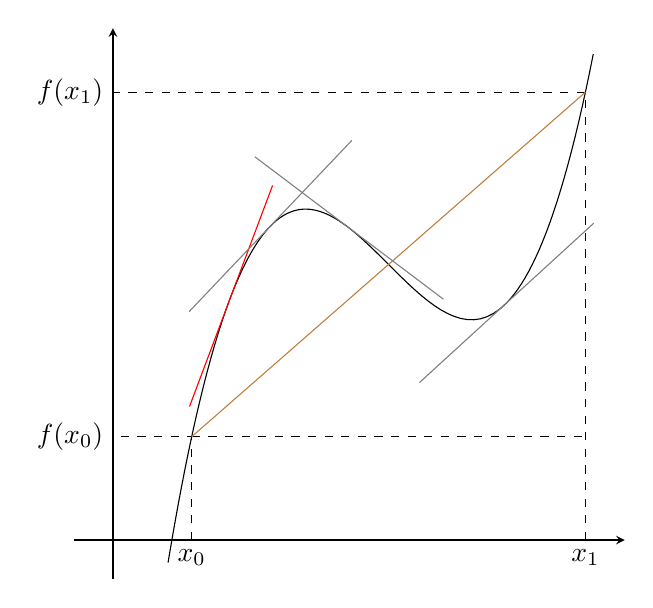
\begin{tikzpicture}[declare function = {curve(\x)=0.3*(\x-3.5)^3-\x+7; x_0=1; x_1=6;}]
				% Axes
				\draw[-stealth] (-0.5,0) -- (6.5,0);
				\draw[-stealth] (0,-0.5) -- (0,6.5);
				% Curve
				\draw[domain=.7:1.5] plot (\x,{curve(\x)}) {[turn] (-1.5,0) coordinate(t0) (1.5,0) coordinate(t1)}; % This is the most steep tangent
				\draw[domain=1.5:2] plot (\x,{curve(\x)}) {[turn] (-1.5,0) coordinate(t2) (1.5,0) coordinate(t3)};
				\draw[domain=2:3] plot (\x,{curve(\x)}) {[turn] (-1.5,0) coordinate(t4) (1.5,0) coordinate(t5)};
				\draw[domain=3:5] plot (\x,{curve(\x)}) {[turn] (-1.5,0) coordinate(t6) (1.5,0) coordinate(t7)};
				\draw[domain=5:6.1] plot (\x,{curve(\x)});
				% Dashed lines
				\foreach \x in {x_0,x_1}
				{\draw[dashed] (\x,0) node[below]{$\x$} |- (0,{curve(\x)}) node[left] {$f(\x)$};}
				\draw[dashed] (x_0,{curve(x_0)}) -- (x_1,{curve(x_0)});
				% Delta-y
				\draw[brown] ({x_0},{curve(x_0)}) -- ({x_1},{curve(x_1)});
				% Tangents
				\draw[red] (t0)--(t1);
				\draw[black!50] (t2)--(t3);
				\draw[black!50] (t4)--(t5);
				\draw[black!50] (t6)--(t7);
			\end{tikzpicture}
		\end{center}
	\end{note}
	\begin{proof}
		Si può dare per scontato che $x_1 \neq x_0$, in quanto, se $x_1 = x_0$ , allora $f(x_1) = f(x_0)$ e la \cref{eq:accresc_fin} diventerebbe $0 \leq 0$. La tesi sarebbe quindi verificata direttamente.\\
		Fissato un qualsiasi $v \in \R^m$, si definisce così la funzione $F$ legata ad $f$ tramite la \fullref{def:segmento}:
		\begin{equation}
			\label{eq:accresc_fin_F}
			\funcdef{F}{\intervalclose{0}{1}}{\R}{t}{v \cdot f \bigl( t x_1 + (1-t)x_0 \bigr)}
		\end{equation}
		\begin{note}
			Nella \cref{eq:accresc_fin_F},  $\cdot$  è Prodotto Scalare tra due vettori di dimensione $\R^m$, dunque il risultato è correttamente uno scalare.
		\end{note}
		$F$ è continua e derivabile sull'intervallo di definizione $\intervalclose{0}{1}$. È dunque possibile utilizzare il \fullref{teo:lagrange}, che garantisce:
		\[\exists c \in \intervalopen{0}{1}: \quad F(1) - F(0) = F'(c) \; (1-0)\]
		Tornando dunque a $f$ dalla definizione di $F$
		\[v \cdot f(x_1) - v \cdot f(x_0) = v \cdot Df\bigl( cx_1 + (1-c)x_0 \bigr) (x_1 - x_0)\]
		Ricordando che la $F$ è a valori in $\R$, si può calcolare il valore assoluto mantenendo l'uguaglianza
		\[\abs{v \cdot f(x_1) - v \cdot f(x_0)} = \abs{v \cdot Df\bigl( cx_1 + (1-c)x_0 \bigr) (x_1 - x_0)}\]
		Essendo il secondo membro il valore assoluto di un prodotto scalare, si può applicare ad esso la \textbf{Disuguaglianza di Cauchy-Schwarz} ed ottenere
		\[\abs{v \cdot \bigl( f(x_1) - f(x_0) \bigr)} \leq \norm{v} \cdot \norm{Df\bigl( cx_1 + (1-c)x_0 \bigr) (x_1 - x_0)}\]
		Dunque, seaparando ulteriorimente le norme si arriva alla:
		\begin{equation}
			\label{eq:accr_fin_norm}
			\abs{v \cdot \bigl( f(x_1) - f(x_0) \bigr)} \leq \norm{v} \cdot \norm{Df\bigl( cx_1 + (1-c)x_0 \bigr)} \cdot \norm{x_1 - x_0}
		\end{equation}

		Essendo, come detto all'inzio, $f(x_1) \neq f(x_0)$ è ora possibile scegliere un $v$ "comodo", come:
		\[v = \frac{1}{\norm{f(x_1) - f(x_0)}} \cdot \bigl( f(x_1) - f(x_0) \bigr)\]
		\begin{note}
			La norma di $v$, grazie poi alla proprietà 4 da \fullref{def:norma}, è
			\begin{align*}
				\norm{v} &= \norm{
					\underbrace{\frac{1}{\norm{f(x_1) - f(x_0)}}}_{\text{Scalare}}
					\cdot
					\underbrace{\bigl( f(x_1) - f(x_0) \bigr)}_{\text{Vettore}}
					}\\
				&= \abs{\frac{1}{\norm{f(x_1) - f(x_0)}}} \cdot \norm{\bigl( f(x_1) - f(x_0) \bigr)}\\
				&= \frac{1}{\norm{f(x_1) - f(x_0)}} \cdot \norm{\bigl( f(x_1) - f(x_0) \bigr)}\\
				&= 1
			\end{align*}
		\end{note}
		Sostituendo dunque in \cref{eq:accr_fin_norm} si ottiene
		\[\norm{\frac{1}{\norm{f(x_1) - f(x_0)}} \cdot \bigl( f(x_1) - f(x_0) \bigr) \cdot \bigl( f(x_1) - f(x_0) \bigr)} \leq \cdot \norm{Df\bigl( cx_1 + (1-c)x_0 \bigr)} \cdot \norm{x_1 - x_0}\]
		Dal punto 3 di \fullref{ex:sp_norm}, si ottiene
		\[\norm{\frac{1}{\norm{f(x_1) - f(x_0)}} \cdot \norm{f(x_1) - f(x_0)}^2} \leq \norm{Df\bigl( cx_1 + (1-c)x_0 \bigr)} \cdot \norm{x_1 - x_0}\]
		Da cui
		\[\norm{f(x_1) - f(x_0)} \leq \norm{Df\bigl( cx_1 + (1-c)x_0 \bigr)} \cdot \norm{x_1 - x_0}\]
		e passando al $\sup$ su $t \in \intervalopen{0}{1}$ si ottiene la tesi.
	\end{proof}
\end{theorem}
Il seguente esercizio mostra come il \fullref{teo:lagrange} non possa essere esteso al caso di funzioni a valori in $\R^n$ con $n > 1$.
\begin{exercise}
	Sia $f: \R \to \R^2$ data da $f(t) = (\cos t, \sin t)$. Mostrare che non esiste nessun numero reale $c$ tale che
	\[f(2 \pi) - f(0) = Df(c) \cdot 2 \pi\]
\end{exercise}

\begin{definition}[Insieme Convesso]
	\label{def:convesso}
	Sia $C \subseteq \R^n$
	\begin{equation*}
		\begin{gathered}
			C \text{ è \textbf{Convesso}}\\
			\bydef\\
			\forall x_0,y_1 \in C \quad \brackets{tx_1+(1-t)x_0:\; t \in \intervalclose{0}{1}} \subseteq C
		\end{gathered}
	\end{equation*}
	Cioè un insieme è Convesso se, dati qualsiasi due suoi punti, contiene anche il segmento che li congiunge.
\end{definition}
\begin{exercise}
	Dimostrare la \fullref{prop:convesso_deriv_par_lim_allora_lips}
	% TODO solution
\end{exercise}
\begin{exercise}
	In $\R^n$ dimostrare che ogni segmento è convesso, così come anche ogni sfera.\\
	Esibire un esempio di insieme non convesso.
	% TODO solution
\end{exercise}
\begin{corollary}
	\label{coro:convess_nabla_0_f_const}
	Siano $A \subseteq \R^n$ e $f: A \to \R$
	\[
		\left.
			\begin{array}{l}
				A \text{ \textbf{Aperto Convesso}}\\
				f \text{ \textbf{Differenziabile} in } A\\
				\forall x \in A \quad \nabla f(x) = 0
			\end{array}
		\right\}
		\implies\\
		f \text{ è \textbf{Costante} su } A
	\]
	\vspace*{-\baselineskip}
	\begin{note}
		Come da \fullref{obs:matr_deriv_tot}, $\nabla f(x) = Df(x) \in \mat (1 \times n)$, cioè un vettore riga.
	\end{note}
	\begin{proof}
		Se $\nabla f(x) = Df(x) = 0$, la \cref{eq:accresc_fin} da \fullref{teo:accresc_fin} diventa
		\begin{equation*}
			\begin{gathered}
				\norm{f(x_1) - f(x_0)} \leq \sup\limits_{\xi \in S} 0 \cdot \norm{x_1-x_0}\\
				\norm{f(x_1) - f(x_0)} \leq 0\\
				f(x_1) = f(x_0)
			\end{gathered}
		\end{equation*}
	\end{proof}
\end{corollary}
\begin{exercise}
	Dimostrare che un insieme \textbf{Convesso} è anche \textbf{Connesso}.\\
	Esibire un controesempio al viceversa.
	\begin{solution}
		Supponendo, per assurdo, $C \in \R^n$ sconnesso. In questo caso, per \fullref{def:connesso}, esistono due insiemi separati $S_1$ e $S_2$ che costituiscono $C$, inoltre $S_1 \cup S_2 = C$ e $S_1 \cap S_2 = \emptyset$. Questo implica che
		\[\exists t \in \intervalclose{0}{1}:\; \forall x_1 \in S_1 \text{ e } \forall x_2 \in S_2 \quad tx_1 + (1-t)x_2 \notin S_1 \text{ e contemporaneamente } \notin S_2\]
		Questo implica la non convessità di $C$ - \textit{Assurdo}.
	\end{solution}
	\begin{solution}
		Preso il cerchio di raggio unitario $S = {(x,y): x^2 + y^2 = 1}$, questo verifica la \fullref{def:connesso} ma sicuramente non la \fullref{def:convesso}.
	\end{solution}
\end{exercise}
\begin{exercise}
	Esibire esempi di insiemi convessi/non convessi e aperti/chiusi, limitati/illimitati.
	% TODO solution
\end{exercise}

\begin{definition}[Funzione Convessa]
	Sia $I$ un intervallo reale e $f:\; I \to \R$.
	\begin{equation*}
		f \text{ è \textbf{Convessa}}
		\quad \bydef \quad
		\begin{cases}
			\forall x_0, x_1 \in I,\; \forall t \in \intervalclose{0}{1}\\
			f \bigl( (1-t)x_0 + t x_1 \bigr) \leq (1-t) f(x_0) + t f(x_1)
		\end{cases}
	\end{equation*}
	Cioè se il segmento che congiunge due qualsiasi punti del suo grafico si trova al di sopra del grafico stesso.
\end{definition}
\begin{exercise}
	Verificare che $f$ è \textbf{Convessa} se e solo se il suo \textbf{Epigrafo} (cioè l'insieme di punti che stanno al di sopra o sul grafico della funzione)
	è un sottoinsieme \textbf{Convesso} di $\R^2$ nel senso della \fullref{def:convesso}.
	% TODO solution
\end{exercise}
\begin{proposition}
	Siano $A \subseteq \R^n$ e $f: A \to \R$
	\[
		\left.
			\begin{array}{l}
				A \text{ \textbf{Aperto Connesso}}\\
				f \text{ \textbf{Differenziabile} in } A\\
				\forall x \in A \quad \nabla f(x) = 0
			\end{array}
		\right\}
		\implies\\
		f \text{ è \textbf{Costante} su } A
	\]
	\vspace*{-\baselineskip}
	\begin{note}
		Si sta parlando di insiemi Co\textbf{nn}essi
	\end{note}
	\begin{proof}
		Sia $x_0 \in A$. Per la \fullref{prop:polig_in_aperto_connesso}, ogni punto $x \in A$ può essere unito a $x_0$ con una poligonale interamente contenuta in $A$ dai lati paralleli agli assi. A questo punto è possibile applicare il \fullref{teo:accresc_fin} ad ogni segmento della poligonale ed, essendo $\nabla f(x) = 0$, come in \fullref{coro:convess_nabla_0_f_const}, la $f$ è costante.
	\end{proof}
\end{proposition}

\newpage
\section{Derivate Seconde}
Quanto detto circa le derivate prime può essere ripetuto introducendo derivate di ordine superiore.
\begin{definition}[Derivate Parziali Seconde]
	Sia $f: A \to \R^m$ con $A \subseteq \R^n$ derivabile parzialmente in $x_0$ lungo $e_i$.\\
	Se la funzione $\frac{\partial f}{\partial x_i}$ è a sua volta derivabile parzialmente in $x_0$, questa volta lungo $e_j$, allora la quantità
	\[
		\frac{\partial}{\partial x_j} \frac{\partial f}{\partial x_i} (x_0)
		\quad \bydef \quad
		\begin{array}{c}
			\text{ è la \textbf{Derivata Parziale Seconda}}\\
			\text{di } f \text{ in } x_0 \text{ rispetto a } x_j, x_i \text{ (in quest'ordine)}
		\end{array}
	\]
	e si indica con
	\[\boldsymbol{\frac{\partial^2 f}{\partial x_j \partial x_i} (x_0)}\]
	\vspace*{-\baselineskip}
	\begin{note}
		Altre notazioni comunemente utilizzate per le derivate parziali secone sono: $D^2_{x_j x_i} f$, $\partial^2_{ji} f$, $\partial_{x_j x_i} f$, $f_{x_j x_i}$, $f_{ji}$
	\end{note}
	\begin{note}
		L'ordine qui utilizzato, cioè
		\[\frac{\partial^2 f}{\partial x_j \partial x_i} = \frac{\partial}{\partial x_j} \frac{\partial f}{\partial x_i} \qquad i,j = 1,\:\dotsc\:,n\]
		non è sempre condiviso da tutti i testi di Analisi Matematica.
	\end{note}
\end{definition}
\begin{observation}
	Le regole di derivazione fornite in \fullref{sect:regole_deriv} sono adeguate anche per il calcolo delle Derivate Seconde.
\end{observation}
\begin{exercise}
	\label{ex:num_deriv_sec}
	Siano $A \subseteq \R^n$ e $f:A \to \R^m$. Ammesso che esistano tutte, quante sono le derivate parziali seconde di $f$ in un qualche punto $x_0$?\\
	Confrontare quanto ottenuto con il caso $n = m = 1$ di Analisi 1.
	\begin{solution}
		Ognuna delle $n$ derivate di $f$ ha, a sua volta, $n$ derivate, di conseguenza il numero di derivate seconde di $f$ è $n^2$. Nel caso di Analisi 1, le derivate seconde erano $1^2 = 1$
	\end{solution}
\end{exercise}

\begin{definition}[Differenziale Seconda]
	\label{def:differenz_second}
	Siano $A \subseteq \R^n$, $f:A \to \R^m$ e $x_0 \in \circdot{A}$
	\[
		f \text{ è \textbf{Differenziabile} } 2 \text{ volte in } x_0
		\quad \bydef \quad
		\begin{cases}
			\text{
				\begin{tabular}{c}
					$f$ è \textbf{Differenziabile} in un intorno di $x_0$\\
					\textit{e}\\
					$f'$ è \textbf{Differenziabile} in $x_0$
				\end{tabular}
			}
		\end{cases}
	\]
	Dove $f'$ è una funzione definita in un intorno di $x_0$ a valori in $\mat(m \times n) \in \R^{mn}$.
	\begin{note}
		Questa definizione è utilizzata comunemenete nel linguaggio parlato, ma viene raramente formalizzata come definizione.
	\end{note}
	\begin{note}
		Avendo una funzione	\textit{scalare} $f: A \to \R$ con $A \subseteq \boldsymbol{\R^n}$, la sua derivata prima è un \textit{vettore}. La derivata seconda sarà una \textit{matrice} e così via.
	\end{note}
\end{definition}

\begin{definition}[Matrice Hessiana]
	\label{def:hessiana}
	Siano $A \subseteq \R^n$, $f:A \to \R^m$ e $x_0 \in \circdot{A}$, inoltre $f$ ammette tutte le Derivate Parziali Seconde in $x_0$.\\
	La matrice di queste derivate seconde si chiama \textbf{Matrice Hessiana} di $f$ in $x_0$ e si indica con $\boldsymbol{H_f(x_0)}$
	\[
		H_f(x_0) = D^2f(x_0) =
		\begin{bmatrix}
			\dfrac{\partial^2 f}{\partial x_1 \partial x_1} & \dfrac{\partial^2 f}{\partial x_2 \partial x_1} & \dots & \dfrac{\partial^2 f}{\partial x_n \partial x_1}\\[3ex]
			\dfrac{\partial^2 f}{\partial x_1 \partial x_2} & \dfrac{\partial^2 f}{\partial x_2 \partial x_2} & \dots & \dfrac{\partial^2 f}{\partial x_n \partial x_2}\\[3ex]
			\vdots & \vdots & \ddots & \vdots\\[3ex]
			\dfrac{\partial^2 f}{\partial x_1 \partial x_n} & \dfrac{\partial^2 f}{\partial x_2 \partial x_n} & \dots & \dfrac{\partial^2 f}{\partial x_n \partial x_n}
		\end{bmatrix}
	\]
	\begin{note}
		La Matrice Hessiana non va confusa con la Matrice Jacobiana da \fullref{obs:matr_deriv_tot}, quest'ultima infatti è la matrice delle Derivate Parziali \textbf{Prime}, mentre la Hessiana contiene le \textbf{Seconde}.
	\end{note}
\end{definition}

\subsection{Il Lemma di Schwarz}
\begin{lemma}[di Schwarz]
	\label{lemma:schwarz}
	Siano $A \subseteq \R^2$, $f:A \to \R^m$ e $(x_0, y_0) \in \circdot{A}$. Se $\frac{\partial^2 f}{\partial x \partial y}$ e $\frac{\partial^2 f}{\partial y \partial x}$ \textbf{esistono} in un intorno di $(x_0, y_0)$ e sono \textbf{Continue} in $(x_0, y_0)$, allora
	\[\frac{\partial^2 f}{\partial x \partial y} \quad = \quad \frac{\partial^2 f}{\partial y \partial x}\]
	\begin{proof}
		Scelti $h, k \in \R$ sufficientemente piccoli, in modo tale che le derivate parziali di $f$ siano definite in tutto il rettangolo di estremi
		\[(x_0, y_0) \qquad\qquad (x_0 + h, y_0) \qquad\qquad (x_0, y_0 + k) \qquad\qquad (x_0 + h, y_0 + k)\]
		\begin{center}
			\begin{tikzpicture}
				\pgfmathsetmacro\MAX{8}
				\pgfmathsetmacro\XZ{\MAX / 3 }
				\pgfmathsetmacro\YZ{\MAX / 3 }
				\pgfmathsetmacro\XZh{\MAX / 3 *2}
				\pgfmathsetmacro\YZk{\MAX / 3 *2}
				\coordinate (X0Y0) at (\XZ,\YZ);
				\coordinate (X0hY0) at (\XZh,\YZ);
				\coordinate (X0Y0k) at (\XZ,\YZk);
				\coordinate (X0hY0k) at (\XZh,\YZk);

				\draw[->] (0,0) -- (\MAX,0) node[anchor=north west] {$x$};
				\draw[->] (0,0) -- (0,\MAX) node[anchor=south east] {$y$};
				\draw[dotted] (\XZ,0) -- (\XZ,\MAX);
				\draw[dotted] (0,\YZ) -- (\MAX,\YZ);
				\draw[dotted] (\XZh,0) -- (\XZh,\MAX);
				\draw[dotted] (0,\YZk) -- (\MAX,\YZk);
				\draw node[anchor=north] at (\XZ,0) {$x_0$};
				\draw node[anchor=north] at (\XZh,0) {$x_0+h$};
				\draw node[anchor=east] at (0,\YZ) {$y_0$};
				\draw node[anchor=east] at (0,\YZk) {$y_0+k$};
				\draw node at (X0Y0) {$\bullet$};
				\draw node at (X0Y0k) {$\bullet$};
				\draw node at (X0hY0) {$\bullet$};
				\draw node at (X0hY0k) {$\bullet$};
			\end{tikzpicture}
		\end{center}
		Per come son state scelte $h$ e $k$, è possibile definire sicuramente la quantità
		\[q = f(x_0 + h, y_0 + k) - f(x_0 + h, y_0) - f(x_0, y_0 + k) + f(x_0, y_0)\]
		Per dimostrare la tesi si può ora verificare che la $q$, calcolata lungo percorsi differenti fornisce lo stesso risultato. È possibile fare ciò riconducendo la $q$ a due diverse funzioni in una sola variabile ed applicando il \fullref{teo:lagrange} due volte ad ognuna di esse.
		\begin{enumerate}
			\item Posta $\varphi(\xi) = f(x_0 + \xi, y_0 + k) - f(x_0 + \xi, y_0)$, si ottiene, riordinando i termini della $q$
				\begin{align*}
					q &= \Bigl( f(x_0 + h, y_0 + k) - f(x_0 + h, y_0) \Bigr) - \Bigl( f(x_0, y_0 + k) + f(x_0, y_0) \Bigr)\\
					&= \varphi(h) - \varphi(0)
					\shortintertext{Applicando Lagrange}
					&= h\: \varphi'(\alpha' h)
					\shortintertext{Grazie alla \fullref{prop:diff_somma_diff} si passa alle derivate parziali rispetto a $x$ (la $y$ è fissa)}
					&= h \left( \frac{\partial f}{\partial x}(x_0 + \alpha' h, y_0 + k) - \frac{\partial f}{\partial x}(x_0 + \alpha' h, y_0) \right)
					\intertext{Si definisce ora $\Phi(\xi) = \frac{\partial f}{\partial x}(x_0 + \alpha'h, y_0 + \xi)$}
					&= h \bigl( \Phi(k) - \Phi(0) \bigr)
					\shortintertext{Per la $\Phi$ valgono nuovamente le ipotesi di Lagrange, dunque si ottiene}
					&= hk\: \Phi'(\beta' k)\\
					&= hk\: \frac{\partial^2 f}{\partial y \partial x}(x_0 + \alpha' h, y_0 + \beta' k)
				\end{align*}
			\item Posta $\psi(\xi) = f(x_0 + h, y_0 + \xi) - f(x_0, y_0 + \xi)$, si ottiene, riordinando i termini della $q$
				\begin{align*}
					q &= \Bigl( f(x_0 + h, y_0 + k) - f(x_0, y_0 + k) \Bigr) - \Bigl( f(x_0 + h, y_0) + f(x_0, y_0) \Bigr)\\
					&= \psi(k) - \psi(0)
					\shortintertext{Applicando Lagrange}
					&= k\: \psi'(\beta'' k)
					\shortintertext{Grazie alla \fullref{prop:diff_somma_diff} si passa alle derivate parziali rispetto a $y$ (la $x$ è fissa)}
					&= k \left( \frac{\partial f}{\partial y}(x_0 + h, y_0 + \beta'' k) - \frac{\partial f}{\partial y}(x_0, y_0 + \beta'' k) \right)
					\intertext{Si definisce ora $\Psi(\xi) = \frac{\partial f}{\partial y}(x_0 + \xi, y_0 + \beta'' k)$}
					&= k \bigl( \Psi(k) - \Psi(0) \bigr)
					\shortintertext{Per la $\Psi$ valgono nuovamente le ipotesi di Lagrange, dunque derivando rispetto a $x$ si ottiene}
					&= kh\: \Psi'(\alpha'' h)\\
					&= kh\: \frac{\partial^2 f}{\partial x \partial y}(x_0 + \alpha'' h, y_0 + \beta'' k)
				\end{align*}
		\end{enumerate}
		Si è quindi giunti a due diverse formulazioni di $q$ per degli $\alpha', \alpha'', \beta', \beta'' \in \intervalopen{0}{1}$
		\[\cancel{hk}\: \frac{\partial^2 f}{\partial y \partial x}(x_0 + \alpha' h, y_0 + \beta' k) = \cancel{kh}\: \frac{\partial^2 f}{\partial x \partial y}(x_0 + \alpha'' h, y_0 + \beta'' k)\]
		A questo punto si calcola il limite per $(h, k) \to (0, 0)$. Spostandosi, anche $\alpha', \alpha'', \beta', \beta''$ cambieranno, ma essendo limitati $\in \intervalopen{0}{1}$, non si presentano complicazioni di sorta in quanto vengono moltiplicati per una quantità tendente a zero.
		\[\frac{\partial^2 f}{\partial y \partial x}(x_0, y_0) = \frac{\partial^2 f}{\partial x \partial y}(x_0, y_0)\]
	\end{proof}
\end{lemma}
\begin{observation}
	Il \fullref{lemma:schwarz} ha importanti applicazioni in fisica e nella teoria dei campo. Grazie al lemma è infatti possibile distinguere tra campi \textbf{conservativi} e non: uno dei criteri è appunto il controllo dell'uguaglianza dell derivate parziali miste.
\end{observation}
\begin{exercise}
	Verificare se il \fullref{lemma:schwarz} si applica alla funzione
	\[\funcdef{f}{\R^2}{\R}{(x,y)}{
		\begin{cases}
			\begin{array}{ll}
				\dfrac{x^3 y - xy^3}{x^2 + y^2} & \text{se } (x,y) \neq (0,0)\\
				0 & \text{se } (x,y) = (0,0)
			\end{array}
		\end{cases}
	}\]
\end{exercise}
\begin{corollary}
	Siano $A \subseteq \R^n$, $f:A \to \R^m$ e $x_0 \in \circdot{A}$. Se $\frac{\partial^2 f}{\partial x_i \partial x_j}$ e $\frac{\partial^2 f}{\partial x_j \partial x_i}$ \textbf{esistono} in un intorno di $x_0$ e sono \textbf{Continue} in $x_0$, allora
	\[\frac{\partial^2 f}{\partial x_i \partial x_j} \quad = \quad \frac{\partial^2 f}{\partial x_j \partial x_i}\]
	\begin{proof}
		Segue dal \fullref{lemma:schwarz} applicandolo a tutte le variabili prese 2 a 2.
	\end{proof}
\end{corollary}

\begin{definition}[Funzioni di Classe $\cntclass{2}$]
	Sia $A \subseteq \R^n$ un \textbf{Aperto}.
	\begin{center}
		$\cntclass{1}(A; \R^m)$ è l'insieme delle funzioni $f:A \to \R^m$\\
		con \textbf{tutte} le \textbf{Derivate Parziali seconde continue} in ogni punto di $A$
	\end{center}
	Si può anche leggere \textit{$f$ è di classe $\cntclass{2}$ su $A$ con valori in $\R^m$}.
\end{definition}

\begin{corollary}
	Sia $A \subseteq \R^n$ un aperto.
	\[f \in \cntclass{2}(A;\R) \quad \implies \quad D^2 f \text{ è una matrice \textbf{simmetrica}}\]
	\begin{proof}
		Segue dal \fullref{lemma:schwarz}, in quanto $\frac{\partial^2 f}{\partial x_i \partial x_j} = \frac{\partial^2 f}{\partial x_j \partial x_i}$ per ogni $i, j$ della matrice, andando a verificare la definizione di Matrice Simmetrica.
	\end{proof}
\end{corollary}
\begin{exercise}
	Siano $A \subseteq \R^n$ e $f \in \cntclass{2}(A;\R^m)$.\\
	Quante sono le derivate parziali seconde di $f$ che bisogna necessariamente calcolare? Calcolare questa risposta con quella dell'\fullref{ex:num_deriv_sec}.
	\begin{solution}
		Bisogna calcolare $\frac{n(n+1)}{2}$ derivate diverse, invece che $n^2$.
	\end{solution}
\end{exercise}
\begin{exercise}
	Esibire un esempio di funzione $f:\R^2 \to \R$ che ammetta tutte le derivate parziali seconde in un punto, ma che non sia continua in quel punto
	% TODO solution
\end{exercise}

\subsection{Sviluppo in Serie di Taylor al II Ordine}
\begin{note}
	Differentemente da quanto fatto sul libro, tutte le funzioni in esame saranno a valori in $\R^1$, visto che a lezione è trattato solo questo caso e che il Resto di Lagrange non è applicabile nel caso di $f: \R^n \to \R^m$.
\end{note}
Fino ad ora son stati visti 2 "livelli" di approssimazione di una funzione $f$ in un intorno del punto $x_0$, appartenente all'insieme di definizione di $f$. Per $x \to x_0$:
\begin{itemize}
	\item Livello $0$: \quad $f$ continua \qquad $f(x) = f(x_0) + o(1)$
	\item Livello $1$: \quad $f$ derivabile \qquad $f(x) = f(x_0) + f'(x_0)(x - x_0) + o(x - x_0)$
\end{itemize}
A livello $0$, la funzione è stata approssimata dal \textit{miglior} polinomio di grado $0$, cioè la costante $f(x_0)$; a livello $1$ dal \textit{miglior} polinomio di grado $1$, $f(x) = f(x_0) + f'(x_0)(x - x_0)$. Per \textit{migliore} si intende che usando un qualsiasi altro polinomio di grado $1$ passante per $\bigl( x_0, f(x_0) \bigr)$ il resto sarebbe andato a $0$ come $x - x_0$ e non più velocemente. Queste approssimazioni ci permettono di capire se una funzione sia crescente o meno, ma non è possibile, ad esempio, studiarne la concavità. Per ottenere più informazioni è possibile estendere questi risultati a polinomi di grado superiore al primo.\\
Come nel caso Analisi 1, gli \textbf{Sviluppi di Taylor} permettono di approssimare localmente una funzione con un polinomio nelle variabili indipendenti a patto di conoscere opportune derivate parziali della funzione.

\vspace*{\baselineskip}
\cbstart
La seguente sezione affiancata da una banda verde non è richiesta, in quanto non presentata sul libro. È però necessaria per chiarire i concetti con cui si sta lavorando, deve quindi essere considerata come un approfondimento da leggere.
\begin{definition}[Polinomio di Taylor]
	\label{def:pol_taylor}
	Siano:
	\begin{itemize}[noitemsep]
		\item $f \in \cntclass{n}(A;\R^m)$ con $A \subseteq \R^n$
		\item $x_0 \in \circdot{A}$
		\item $h \in \R^n$
		\item Il segmento di estremi $x_0$ e $x_0 + h$ è interamente contenuto in $A$
	\end{itemize}
	Allora
	\[T_{n-1}(f, x_0) = f(x_0) + Df(x_0; h) + \frac{1}{2!} D^2f(x_0; h) + \cdots + \frac{1}{(n-1)!} D^{n-1}f(x_0; h)\]
	Oppure, in forma più compatta
	\begin{equation}
		\label{eq:pol_taylor}
			T_{n-1}(f, x_0) = \sum\limits_{i = 1}^{n-1} \frac{1}{i!} D^if(x_0; h)
	\end{equation}
	si dice \textbf{Polinomio di Taylor} di grado $n-1$ della funzione $f$ centrato nel punto $x_0$.

	\begin{note}
		Nella \cref{eq:pol_taylor}, con la forma $D^if(x_0; h)$ si intende lo \textit{scalare} ottenuto applicando all’incremento $h$ il differenziale $i$\textit{-esimo} calcolato in $x_0$.\\
		Supponendo $f: R^n \to \R^1$, la $D^if(x_0; h)$ diventa, ad esempio:
		\begin{itemize}
			\item $i = 1 \qquad Df(x_0; h) = \nabla f(x_0) \cdot h$
			\item $i = 2 \qquad D^2f(x_0; h) = h^T \cdot H_f(x_0) \cdot h$ \quad dove $h^T$ è $h$ trasposto e $H_f$ è la \fullref{def:hessiana}
		\end{itemize}
		Con $\; \cdot \;$, in questo caso, si intende il prodotto righe per colonne.\\
		Vedasi \fullref{obs:matr_deriv_tot} per le possibile "forme" assunte dalla $Df(x_0; h)$ in base ai valori di $n$ e $m$.
	\end{note}
\end{definition}
\begin{observation}
	Il Polinomio di Taylor è caratterizzato dall’avere in comune con la funzione $f$ il valore di tutte le derivate fino all’ordine $n-1$ nel punto $x_0$.
\end{observation}
\begin{theorem}[di Taylor]
	\label{teo:taylor}
	Siano:
	\begin{itemize}[noitemsep]
		\item $f \in \cntclass{n}(A;\R^m)$ con $A \subseteq \R^n$
		\item $x_0 \in \circdot{A}$
		\item $h \in \R^n$
		\item Il segmento di estremi $x_0$ e $x_0 + h$ è interamente contenuto in $A$
	\end{itemize}
	Allora
	\[f(x) = T_{n-1}(f, x_0) + R_n(f, x_0, h) \qquad \text{per } x \to x_0\]
	Dove $R_n(f, x_0, h)$ è \textbf{Resto} espresso nella forma di Peano o di Lagrange.
	\begin{proof}
		Omessa.
	\end{proof}
\end{theorem}

\begin{definition}[Resto di Peano]
	\label{def:resto_peano}
	Nelle ipotesi del \fullref{teo:taylor}, dalla \fullref{def:o_piccolo} si definisce il \textbf{resto} nella forma \textbf{di Peano}:
	\[R_n(f, x_0, h) = \frac{1}{n!} D^nf(x_0; h) + o\left( \norm{h}^2 \right)\]
	Cioè che la differenza tra la funzione ed il polinomio tende a zero quando la $x$ tende al centro dello sviluppo, cioè $x_0$
\end{definition}

\begin{definition}[Resto di Lagrange]
	Nelle ipotesi del \fullref{teo:taylor}, ma con $f \in \cntclass{n}(A;\R^{\boldsymbol{1}})$ si definisce il \textbf{resto} nella forma \textbf{di Lagrange}
	\[\exists \theta \in \intervalclose{0}{1}: \quad R_n(f, x_0, h) = \frac{1}{n!} D^nf(x_0; \theta h) = \frac{D^n f(x + \theta h)}{n!} (x + \theta h)\]
	Cioè che esiste un punto (senza sapere quale sia) all'interno del segmento di estremi $x_0$ e $x_0 + h$ in cui si ha un'equivalenza precisa tra la funzione ed il polinomio.
\end{definition}
\begin{observation}
	\label{obs:resto_lagr_Rn}
	Il Resto di Lagrange, a differenza del \fullref{def:resto_peano}, offre informazioni quantitative sul resto, ma \textbf{NON} è applicabile a funzioni a valori in $\R^m$, solo a funzioni a valori reali.
\end{observation}
\cbend

\noindent Passando ora al caso specifico degli sviluppi del secondo ordine
\begin{proposition}[Sviluppo di Taylor al Secondo Ordine con resto di Peano]
	\label{prop:svil_tay_2_peano}
	Siano:
	\begin{itemize}[noitemsep]
		\item $f \in \cntclass{2}(A;\R^m)$ con $A \subseteq \R^n$
		\item $x_0 \in \circdot{A}$
		\item $h \in \R^n$
		\item Il segmento di estremi $x_0$ e $x = x_0 + h$ è interamente contenuto in $A$
	\end{itemize}
	Allora
	\[f(x) = f(x_0) + Df(x_0)h + \frac{1}{2} h^T D^2f(x_0) h + o\left( \norm{h}^2 \right)\]
	\begin{note}
		$h^T$ è il vettore riga trasposto del vettore colonna $h$.
	\end{note}
	\begin{proof}
		Omessa in aula.
	\end{proof}
\end{proposition}

\begin{proposition}[Sviluppo di Taylor al Secondo Ordine con resto di Lagrange]
	Siano:
	\begin{itemize}[noitemsep]
		\item $f \in \cntclass{2}(A;\R)$ con $A \subseteq \R^n$
		\item $x_0 \in \circdot{A}$
		\item $h \in \R^n$
		\item Il segmento di estremi $x_0$ e $x_0 + h$ è interamente contenuto in $A$
	\end{itemize}
	Allora
	\[f(x) = f(x_0) + Df(x_0)h + \frac{1}{2} h^T D^n f(x + \theta h) h\] % TODO chehck this formula
	\begin{note}
		Come detto in \fullref{obs:resto_lagr_Rn}, il resto di lagrange si può applicare solo a funzioni in $\R$.
	\end{note}
	\begin{proof}
		Omessa in aula.
	\end{proof}
\end{proposition}

\begin{exercise}
	Sfruttando i noti sviluppi di funzioni reali di una variabile reale, scrivere lo sviluppo di Taylor al secondo ordine centrato nell'origine delle seguenti funzioni:
	\begin{itemize}
		\begin{minipage}{0.33\linewidth}
			\item $(x,y) \mapsto 2x^2 + 3xy + 4xy^3$
			\item $(x,y) \mapsto \sin(xy)$
			\item $(x,y,z) \mapsto (x+z) \cos (2x+3y)$
		\end{minipage}
		\begin{minipage}{0.33\linewidth}
			\item $(x,y) \mapsto e^{x-y^2} \ln(1+x+y^2)$
			\item $(x,y,z) \mapsto \sqrt{1+2x+3y+4z}$
			\item $(x,y) \mapsto \begin{bmatrix}
					\cos(x^2 + y^2)\\
					\sin(x^2 - y^2)
				\end{bmatrix}$
		\end{minipage}
		\begin{minipage}{0.33\linewidth}
			\item $(x,y,z) \mapsto \sin(x + 3z) \cos(z - y)$
			\item $(x,y) \mapsto \frac{x+y^2}{\cos (x+y)}$
			\item $(x,y,z) \mapsto \begin{bmatrix}
					z \ln (1 + xy)\\
					\frac{y}{1+x+z}\\
					(y + z) \sin x
				\end{bmatrix}$
		\end{minipage}
	\end{itemize}
\end{exercise}

\subsection{Derivate di Ordine Superiore}
\begin{definition}
	Sia $k \in \N$ e sia $A \subseteq \R^n$ un \textbf{Aperto}. $\cntclass{0}(A;\R^m)$ è l'insieme delle funzioni continue su $A$ con valori in $\R^m$. Se $k \geq 1$, $\cntclass{k}(A;\R^m)$ è l'insieme delle funzioni continue su $A$ con valori in $\R^m$ con tutte le derivate parziali prime di classe $\cntclass{k-1}$ su $A$.\\
	Inoltre
	\[\cntclass{\infty}(A;\R^m) = \bigcap\limits_{k \in \N}\cntclass{k}(A;\R^m)\]
	Si può anche leggere \textit{$f$ è di classe $\cntclass{k}$ o $\cntclass{\infty}$ su $A$ con valori in $\R^m$}.
\end{definition}
\begin{exercise}
	Siano $A \subseteq \R^n$ ed $f \in \cntclass{3}(A;\R^m)$. Quante sono le derivate parziali terze di $f$ in totale? E quante quelle che, in generale, bisogna necessariamente calcolare?
	% TODO solution
\end{exercise}

\newpage
\section{Il Teorema della Funzione Implicita}
I risultati esposti in questo paragrafo permettono di studiare funzioni senza averne l'espressione analitica esplicita a disposizione, fatto estremamente importante per l'utilizzo reale dell'analisi. Non è infatti sempre possibile ottenere la forma analitica di una funzione, ma ci può comunque essere necessità di studiarla.
\begin{definition}[Funzione Implicita]
	\label{def:funz_impl}
	Dati
	\begin{itemize}[noitemsep]
		\item $X \subseteq \R^n, Y \subseteq \R^m$
		\item $f: X \times Y \to \R^l$
		\item $(x_0, y_0) \in X \times Y$ (un punto)
	\end{itemize}
	Si dice che l'equazione $f(x,y) = 0$ \textbf{Definisce Implicitamente una Funzione} $\varphi$ in un intorno di $(x_0,y_0)$ se:
	\begin{enumerate}
		\item $f(x_0,y_0) = 0$
		\item Esistono due aperti $\mathcal{X}$ e $\mathcal{Y}$ tali che:
			\begin{itemize}[noitemsep, topsep=0pt]
				\item $x_0 \in \mathcal{X} \subseteq X$
				\item $y_0 \in \mathcal{Y} \subseteq Y$
			\end{itemize}
			\begin{note}
				Oppure, alternativamente, $x_0 \in \circdot{\mathcal{X}}$ e $y_0 \in \circdot{\mathcal{Y}}$ con $\mathcal{X}$ e $\mathcal{Y}$ non aperti.
			\end{note}\vspace*{-2ex}
		\item Esiste $\varphi: \mathcal{X} \to \mathcal{Y}$
	\end{enumerate}
	Tali che:
	\[
		\left.
		\begin{array}{l}
			x \in \mathcal{X}\\
			y \in \mathcal{Y}\\
			f(x,y) = 0
		\end{array}
		\right\}
		\implies
		y = \varphi(x)
	\]
	Con $\varphi$ \textbf{Funzione Implicita} definita da $f(x,y)=0$.\\

	Cioè la Funzione Implicita associa un sottoinsieme delle variabili dell'equazione alle variabili rimanenti. Da questo deriva il nome \textit{implicita}, in quanto la $f$ definisce "implicitamente" la $\varphi$, perchè l'immagine di $f$ è influenzata da tutte le variabili della funzione, che dunque son legate tra loro.
	\begin{note}
		La \textbf{Funzione Inversa} di una qualche funzione è anche \textbf{Funzione Implicita} di questa funzione.
	\end{note}
\end{definition}
\begin{example}
	Posti $m = n = l = 1$
	\[\funcdef{f}{\R \times \R}{\R}{(x,y)}{x^2 + y^2 + 1}\]
	Non definisce alcuna funzione implicita poiché $f(x,y) = 0$ non è mai verificata.
\end{example}
\begin{example}
	Posti $m = n = l = 1$
	\[\funcdef{f}{\R \times \R}{\R}{(x,y)}{x^2 + y^2 - 1}\]
	\begin{note}
		Il Teorema della Funzione Implicita è particolarmente utile quando non è possibile esprimere in forma analitica un parametro rispetto agli altri, ma è ovviamente utilizzabile anche quando è fattibile.
	\end{note}
	Per prima cosa si osserva che è possibile trovare dei punti che verifichino l'uguaglianza $f(x,y) = 0$, cioè tutti i punti della circonferenza di raggio unitario centrata nell'origine. Il punto $(0,1)$ definisce implicitamente, tra le altre, una funzione
	\begin{equation}
		\label{eq:ese_funz_impl_cerchio}
		\funcdef{\varphi_1}{\intervalopen{-1}{1}}{\R^+}{x}{\sqrt{1-x^2}}
	\end{equation}
	\begin{note}
		$\varphi_1$ non avrebbe potuto essere definita $\intervalopen{-1}{1} \to \intervalopcl{0}{1}$ perché sarebbe contrario al punto 2 della \fullref{def:funz_impl}, non essendo $\mathcal{Y}$ un aperto, in questo caso. Estendendo $\mathcal{Y}$ a $\R^+$ si ha un aperto contenente tutti i valori assunti da $\varphi_1$.
	\end{note}
	Un primo problema nasce dalla scelta degli insiemi $\mathcal{X}$ e $\mathcal{Y}$, per esempio sarebbero stati altrettanto accettabili $\mathcal{X} = \intervalopen{-\frac{1}{2}}{\frac{1}{2}}$ e $\mathcal{Y} = R^+ $. Un secondo problema è la scelta del punto nel cui intorno si cercherà la funzione implicita: sarebbe stato possibile scegliere il punto $(\frac{1}{\sqrt{2}},\frac{1}{\sqrt{2}})$ oppure ancora $(-\frac{1}{2},-\frac{\sqrt{3}}{2})$. Sicuramente $(1,0)$ non è un punto valido, dato che non si verifica il punto 3 della \fullref{def:funz_impl}, perché una eventuale relazione come $\varphi_3$ da \autoref{fig:ese_funz_impl_cerchio} non sarebbe una funzione.
	\begin{note}
		La $\varphi_1$ di \cref{eq:ese_funz_impl_cerchio} potrebbe essere scritta in funzione di $y$ poiché, a priori, non c'è distinzione tra le variabili.
	\end{note}
	~
	\begin{figure}[H]
		\caption{Esempi di funzioni implicite della $f$}
		\label{fig:ese_funz_impl_cerchio}
		\centering
		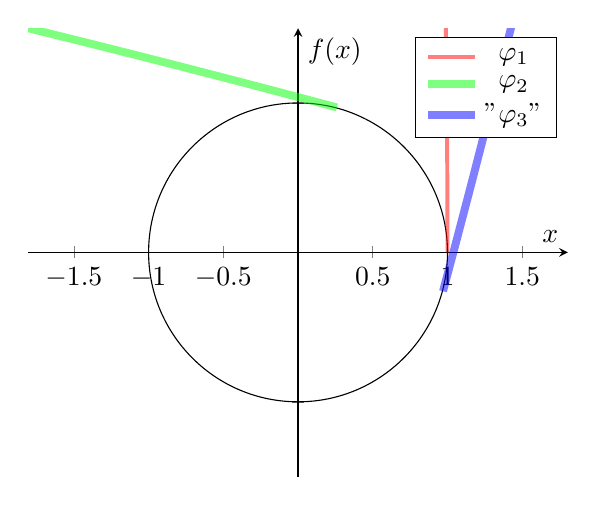
\begin{tikzpicture}
			\begin{axis}[
				axis lines = center,
				xmin=-1.5, xmax=1.5, ymin=-1.5, ymax=1.5,
				axis equal,
				xlabel = $x$,
				ylabel = {$f(x)$},
				yticklabels={,,}
			]
			\draw (axis cs: 0, 0) circle [radius=1];
			\draw[line width=.5mm, red, opacity=.5] (axis cs: 1, 0) arc [radius=100, start angle=0, end angle=180];
			\addlegendimage{line width=.5mm, opacity=.5, color=red}
			\addlegendentry{$\varphi_1$}
			\draw[line width=1mm, green, opacity=.5] (axis cs: .26, .97) arc [radius=100, start angle=75, end angle=105];
			\addlegendimage{line width=1mm, opacity=.5, color=green}
			\addlegendentry{$\varphi_2$}
			\draw[line width=1mm, blue, opacity=.5] (axis cs: .97, -.26) arc [radius=100, start angle=-15, end angle=15];
			\addlegendimage{line width=1mm, opacity=.5, color=blue}
			\addlegendentry{"$\varphi_3$"}
			\end{axis}
		\end{tikzpicture}
	\end{figure}
\end{example}
\begin{example}
	Posti $m = n = l = 1$
	\[\funcdef{f}{\R \times \R}{\R}{(x,y)}{x^2 + y^2}\]
	L'uguaglianza $f(x,y) = 0$ non definisce implicitamente alcuna funzione in quanto $\dom f = \brackets{(0,0)}$ che è composto da un solo punto isolato, dunque non esistono $\mathcal{X} \subseteq X$ e $\mathcal{Y} \subseteq Y$ aperti.
\end{example}
\begin{example}
	\label{ex:inf_funz_impl}
	Posti $m = n = l = 1$
	\[\funcdef{f}{\R \times \R}{\R}{(x,y)}{x^2 - y^2}\]
	L'uguaglianza $f(x,y) = 0$ definisce implicitamente infinite funzioni distinte in un intorno di $(0,0)$.
\end{example}
\begin{exercise}
	Determinare (almeno) 5 funzioni diverse definite implicitamente dalla funzione nell'\fullref{ex:inf_funz_impl} sullo stesso insieme
	% TODO solution
\end{exercise}
\begin{example}[Equazione di Keplero]
	Nella meccanica orbitale, l'\textbf{Equazione di Keplero} è un importante risultato che mette in relazione varie proprietà dell'orbita di un oggetto soggetto ad una forza centrale fornendo la legge oraria del suo moto. Dati
	\begin{itemize}[noitemsep]
		\item \makebox[2ex]{$M$\hfill} \textit{Anomalia Media}: frazione di periodo orbitale trascorsa dall'ultimo passaggio al pericentro $z$, espressa come angolo.
		\item \makebox[2ex]{$E$\hfill} \textit{Anomalia Eccentrica}: valore angolare utilizzato per correggere lo scostamento tra l'anomalia vera, cioè quella osservata, e quella media (da sopra)
		\item \makebox[2ex]{$e$\hfill} \textit{Eccentricità} dell'orbita del corpo
		\item \makebox[2ex]{$n$\hfill} \textit{Velocità angolare media} del corpo
		\item \makebox[2ex]{$t$\hfill} \textit{Istante} di tempo in cui si vuol calcolare la posizione del corpo
		\item \makebox[2ex]{$\tau$\hfill} \textit{Istante} di tempo di passaggio per il pericentro (perielio nel caso del Sole)
	\end{itemize}
	Si ha la
	\[\underbrace{E - e \sin(E)}_{= M} = n (t - \tau)\]
	Dalla quale è però impossibile esplicitare la $E$, necessaria per il calcolo della posizione, in funzione del tempo $t$. È possibile, al massimo, avvicinarsi alla soluzione con metodi di approssimazione.
\end{example}

\vspace*{\baselineskip}
Per funzioni lineari il Teorema della Funzione Implicita si riduce alla semplice inversione di una matrice.
\begin{theorem}[della Funzione Implicita - Caso Lineare]
	\label{teo:funz_impl_lin}
	Siano:
	\begin{itemize}[noitemsep]
		\item $A \in \mat(p \times n)$ matrice
		\item $B \in \mat(p \times m)$ matrice
		\item $C \in \mat(p \times 1)$ vettore colonna
		\item $p = m$
		\item $\det(B) \neq 0$
	\end{itemize}
	e la funzione
	\[\funcdef{f}{\R^n \times \R^m}{\R^p}{(x, y)}{Ax + By - C}\]
	Allora esiste un'unica funzione $\varphi: \R^n \to \R^m$ tale che:
	\[Ax + By = C \quad \iff \quad f(x,y) = 0 \quad \iff \quad y = \varphi(x)\]
	\vspace*{-5ex}
	\begin{note}
		Dimensionalmente, avendo $p = m$ ed eseguendo i prodotti righe per colonne, ci si porta ad avere da entrambi i lati dell'uguaglianza matriciale dei vettori colonna $\in \mat(p \times 1)$
	\end{note}
	\begin{proof}
		\begin{align*}
			Ax + By &= C\\
			By &= C - Ax\\
			\shortintertext{Essendo $p = m$ e $\det(B) \neq 0$, la matrice $B$ è invertibile, dunque}
			B^{-1} By &= B^{-1} (C - Ax)\\
			y &= B^{-1} (C - Ax)
		\end{align*}
		Quindi è possibile esprimere la $y$ in funzione della sola $x$, verificando la tesi.
	\end{proof}
\end{theorem}

\begin{observation}[Metodo di Newton, o delle Tangenti]~
	\label{obs:metodo_newton}
	\vspace*{-\baselineskip}
	\begin{note}
		Questo metodo, leggermente modificato, sarà utile nella dimostrazione del \fullref{teo:funz_impl}.
	\end{note}
	Sia $f: \intervalclose{a}{b} \to \R$ con $f \in \cntclass{2}(\intervalclose{a}{b}, \R)$. Se l'intervallo $\intervalclose{a}{b}$ contiene una sola radice della $f$, allora si può individuare la radice per mezzo di successive approssimazioni della curva con le sue tangenti.\\
	Procedendo in modo iterativo si dimostra che la relazione di ricorrenza del metodo è:
	\begin{equation}
		\label{eq:metodo_newton}
		x_{n+1} = x_n - \frac{f(x_n)}{f'(x_n)}
	\end{equation}
	Che è una successione convergente alla radice.\\
	Graficamente si vede come utilizzando le tangenti ci si possa spostare rapidamente verso la radice:
	\begin{center}
		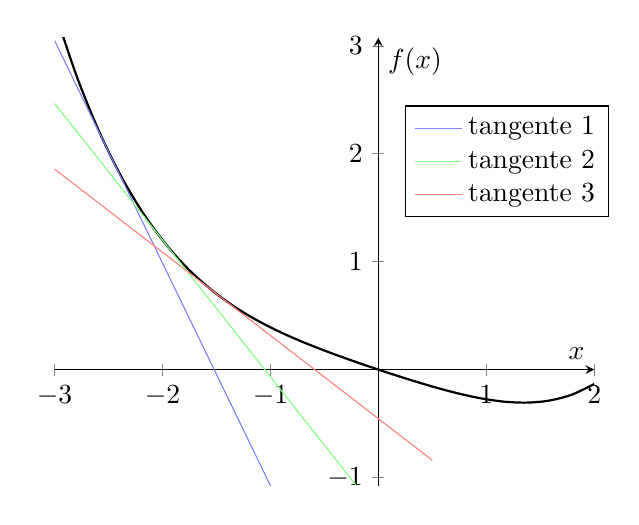
\begin{tikzpicture}[declare function = {curve(\x)=(1/40)*\x^4+(1/30)*\x^2-(1/3)*\x; derivative(\x)=(1/10)*\x^3+(1/15)*\x-(1/3);}]
			\begin{axis}[
				axis lines = center,
				axis equal,
				ymax = 3, ymin = -1,
				xlabel = $x$,
				ylabel = {$f(x)$},
				legend style = {at={(.65,0.6)},anchor=south west}
			]
				\addplot[domain=-3:2, smooth, thick, forget plot] {curve(x)};
				\addplot[domain=-3:.5, color=blue!50]{(x+2.5)*derivative(-2.5) + curve(-2.5)};
				\addlegendentry{tangente 1}
				\addplot[domain=-3:.5, color=green!50]{(x+2)*derivative(-2) + curve(-2)};
				\addlegendentry{tangente 2}
				\addplot[domain=-3:.5, color=red!50]{(x+1.5)*derivative(-1.5) + curve(-1.5)};
				\addlegendentry{tangente 3}
			\end{axis}
		\end{tikzpicture}
	\end{center}
\end{observation}

\begin{theorem}[della Funzione Implicita]~
	\label{teo:funz_impl}
	\vspace*{-\baselineskip}
	\begin{note}
		Questo teorema è anche noto come \textit{Teorema di Dini}
	\end{note}
	Siano:
	\begin{enumerate}[noitemsep]
		\item \label{itm:ipot_funz_impl_1} $X \subseteq \R^n$ e $Y \subseteq \R^m$ \textbf{Aperti}
		\item \label{itm:ipot_funz_impl_2} $f: X \times Y \to \R^m$ e $f$ \textbf{Continua} in $X \times Y$
		\item \label{itm:ipot_funz_impl_3} $(x_0, y_0) \in X \times Y$ e $f(x_0, y_0) = 0$
		\item \label{itm:ipot_funz_impl_4} $D_yf$ \textbf{esiste Continua} in $(x_0, y_0)$
		\item \label{itm:ipot_funz_impl_5} $D_yf(x_0, y_0)$ ammette \textbf{inversa}
	\end{enumerate}
	\begin{note}
		\hypertarget{note:teo_funz_impl_note_ipot1}{}
		Nel \fullref{teo:funz_impl_lin} si utilizzava direttamente la matrice dell'applicazione lineare, mentre qui si ha la la matrice Derivata Totale. Questo perché il differenziale è la funzione che meglio approssima una funzione in un suo punto, permettendo una pseudo linearità malgrado la $f$ non sia (necessariamente) lineare.
	\end{note}
	\begin{note}
		Nei punti \ref{itm:ipot_funz_impl_4} e \ref{itm:ipot_funz_impl_5} delle ipotesi si ha $D_yf$ perché si sta cercando una funzione implicita che esprima la $y$, se la si stesse cercando per la $x$ si dovrebbe utilizzare la $D_xf$
	\end{note}
	\begin{note}
		Il punto \ref{itm:ipot_funz_impl_5} delle ipotesi richiede che la matrice $D_yf$ sia invertibile, cioè quadrata e con $\det(D_yf) \neq 0$. Il fatto che sia quadrata è garantito per ipotesi, in quanto $Y \subseteq \R^m$ e $f$ è a valori in $\R^m$\\
		Nel caso molto comune di $f: \R^1 \times \R^1 \to \R^1$, bisogna verificare che $\frac{\partial f}{\partial y} \neq 0$, cioè che la derivata parziale rispetto ad $y$ non sia nulla.
	\end{note}
	Allora
	\begin{enumerate}
		\item Esistono degli intorni $\mathcal{X}$ di $x_0$ e $\mathcal{Y}$ di $y_0$ ed esiste la \textbf{funzione Continua} $\varphi: \mathcal{X} \to \mathcal{Y}$ tale che, con $x \in \mathcal{X}$ e $y \in \mathcal{Y}$
			\begin{equation}
				\label{eq:teo_funz_impl_f_phi}
				f(x,y) = 0 \quad \iff \quad y = \varphi(x)
			\end{equation}
		\item \label{itm:tesi_funz_impl_1} Se $\varphi_1: \mathcal{X}_1 \to \mathcal{Y}_1$ e $\varphi_2: \mathcal{X}_2 \to \mathcal{Y}_2$ soddisfano alla \cref{eq:teo_funz_impl_f_phi} con $\mathcal{X}_1, \mathcal{X}_2 \subseteq \mathcal{X}$ intorni di $x_0$ e $\mathcal{Y}_1, \mathcal{Y}_2 \subseteq \mathcal{Y}$ intorni di $y_0$, allora
			\[\varphi_1 = \varphi_2 \quad \text{su} \quad \mathcal{X} \cap \mathcal{X}_1 \cap \mathcal{X}_2\]
	\end{enumerate}
	\begin{note}
		Il punto \ref{itm:tesi_funz_impl_1} significa che prendendo due $\varphi$ definite su intervalli diversi, esse assumeranno gli stessi valori nei punti comuni ad entrambi gli intervalli (se esistono). Questa proprietà viene spesso indicata dalla forma "$\varphi$ è unica \textit{localmente}".
	\end{note}
	\begin{proof}
		Analogamente alla \cref{eq:metodo_newton}, passando al caso multidimensionale, si definisce la funzione
		\begin{equation}
			\label{eq:funz_impl_T}
			\funcdef{T}{\mathcal{X} \times \mathcal{Y}}{\mathcal{Y}}{(x,y)}{y - [D_yf(x_0, y_0)]^{-1} \cdot f(x, y)}
		\end{equation}
		\begin{note}
			$[D_yf(x_0, y_0)]^{-1}$ è la matrice inversa della $D_yf$
		\end{note}
		Considerando la $x$ della $T$ come un parametro, si può dire che $T$ sia una \fullref{def:contrazione_parametro}. Bisogna però verificare che sia effettivamente una contrazione, cioè che rispetti due condizioni:
		\begin{enumerate}
			\item \textit{La $T$ esegue una contrazione delle distanze}\\
				Questo si può dimostrare grazie al \fullref{teo:accresc_fin}. Infatti se il $\sup\limits_{\xi \in S} \norm{Df(\xi)}$ dell'\cref{eq:accresc_fin} è un numero $\in \intervalclop{0}{1}$, allora (sostituendo la distanza con la norma per \fullref{def:norma}) la \cref{eq:accresc_fin} diventa comparabile alla \cref{eq:contrazione_parametro}, cioè:
				\[
					\begin{gathered}
						d \bigl( T(x, y_1), T(x, y_2) \bigr) \leq K \cdot d(y_1, y_2)\\
						\iff\\
						\norm{ T(x, y_1) - T(x, y_2) } \leq \sup\limits_{\xi \in S} \norm{D_y T(\xi)} \cdot \norm{y_1 - y_2}
					\end{gathered}
				\]
				Per poter applicare il \fullref{teo:accresc_fin} è necessario che il segmento di estremi $y_1$, $y_2$ sia interamente contenuto nella parte interna dell'insieme di definizione di $T$.\\
				Dato che nell'enunciato del teorema è solo indicata l'esistenza di $\mathcal{X}$ e $\mathcal{Y}$, è possibile scegliere questi insiemi a piacimento. Ponendo dei $r_x$ ed $r_y$ sufficientemente piccoli, saranno accettabili:
				\[\mathcal{X} = \overline{B(x_0, r_x)} \qquad\qquad\qquad \mathcal{Y} = \overline{B(y_0, r_y)}\]
				A questo punto il \fullref{teo:accresc_fin} è applicabile, dunque si procede a quantificare il $\sup\limits_{\xi \in S} \norm{Df(\xi)}$ differenziando rispetto ad $y$ la \cref{eq:funz_impl_T}
				\begin{align*}
					D_yT(x,y) &= \id_Y - \bigl[ D_yf (x_0, y_0) \bigr]^{-1} D_yf (x, y)
					\shortintertext{Essendo $\id_Y = \bigl[ D_yf(x, y)\bigr]^{-1} \cdot D_yf(x, y)$ per qualsiasi $(x, y)$, si ha}
					&= \bigl[ D_yf (x_0, y_0) \bigr]^{-1} \cdot D_yf (x_0, y_0) - \bigl[ D_yf (x_0, y_0) \bigr]^{-1} D_yf (x, y)\\
					&= \bigl[ D_yf (x_0, y_0) \bigr]^{-1} \cdot \bigl[ D_yf (x_0, y_0) - D_yf (x, y) \bigr]
				\end{align*}
				Passando alle norme
				\[\norm{D_yT(x,y)} = \norm{\bigl[ D_yf (x_0, y_0) \bigr]^{-1} \cdot \underbrace{\bigl[ D_yf (x_0, y_0) - D_yf (x, y) \bigr]}_{\text{(1)}} }\]
				Essendo, come detto prima, $r_x$ ed $r_y$ piccoli a piacere, si può presupporre che il fattore indicato come (1) tenda a $0$, essendo una differenza tra funzioni continue (per ipotesi). A questo punto, sicuramente, si può minorare con un valore arbitrario: si sceglie $\frac{1}{2}$ in quanto sarà successivamente "comodo" nel corso della dimostrazione.
				\[\norm{D_yT(x,y)} \leq \frac{1}{2}\]
				Dunque, finalmente, applicando il \fullref{teo:accresc_fin}
				\[\norm{ T(x, y_1) - T(x, y_2) } \leq \frac{1}{2} \cdot \norm{y_1 - y_2}\]
				\qed
			\item \textit{La $T$ è a valori nell'insieme di partenza ($T$ "ben definita")}\\
				Preso un generico $y$, si deve verificare che $\forall y \in \mathcal{Y}:\; T(x,y) \in \mathcal{Y}$ cioè, per come è definito $\mathcal{Y}$, che la distanza tra $T(x,y)$ ed $y_0$, centro della $\overline{B(y_0, r_y)}$, sia minore di $r_y$.\\
				Applicando la disuguaglianza triangolare
				\begin{align*}
					\norm{T(x, y) - y_0} &\leq \norm{\underbrace{T(x, y) - T(x, y_0)}_{\text{(1)}} + \underbrace{\norm{T(x, y_0) - y_0}}_{\text{(2)}}}
					\intertext{Applicando nuovamente il \fullref{teo:accresc_fin} ad (1) ed utilizzando la definizione di $T$ per (2)}
					&\leq \underbrace{\sup\limits_{\xi \in S} \norm{D_y T(\xi)}}_{\text{(3)}} \cdot \underbrace{\norm{y - y_0}}_{\text{(4)}} + \norm{y_0 - [D_yf(x_0, y_0)]^{-1} \cdot f(x, y_0) - y_0}
					\shortintertext{Come dimostrato prima (3) è minorato da $\frac{1}{2}$, mentre (4) corrisponde a $r_y$}
					&\leq \frac{1}{2} r_y + \norm{[D_yf(x_0, y_0)]^{-1} \cdot f(x, y_0)}\\
					&= \frac{1}{2} r_y + \norm{[D_yf(x_0, y_0)]^{-1}} \cdot \norm{f(x, y_0)}\\
					&= \frac{1}{2} r_y + \norm{[D_yf(x_0, y_0)]^{-1}} \cdot \norm{f(x, y_0) - 0}
					\shortintertext{Essendo $f(x_0, y_0) = 0$ per ipotesi}
					&= \frac{1}{2} r_y + \underbrace{\norm{[D_yf(x_0, y_0)]^{-1}} \cdot \norm{f(x, y_0) - f(x_0, y_0)}}_{\text{(5)}}
					\shortintertext{Il termine (5) non dipende da $r_y$, ma solo da $r_x$, dunque scegliendo un $r_x$ sufficientemente piccolo, è possibile minorare nuovamente con}
					&\leq \frac{1}{2} r_y + \frac{1}{2} r_y\\
					&\leq r_y
				\end{align*}
				\qed
		\end{enumerate}
		Si è quindi verificato che la $T$ sia effettivamente una \textbf{Contrazione} per ogni $x \in \mathcal{X}$
		\begin{note}
			L'indipendenza dal parametro deriva dall'aver verificato la \fullref{def:contrazione_parametro}
		\end{note}
		Sfruttando il \fullref{teo:contrazioni_con_para} si può essere certi dell'unicità del punto fisso di $T$. Inoltre, il punto fisso di $T$ è anche radice di $f(x,y) = 0$. Questo si dimostra applicando la \fullref{def:punto_fisso} alla $T$:
		\begin{align*}
			T(x,y) = y \quad &\iff \quad y - [D_yf(x_0, y_0)]^{-1} \cdot f(x, y) = y\\
			&\iff \quad [D_yf(x_0, y_0)]^{-1} \cdot f(x, y) = 0
			\shortintertext{Moltiplicando ambo i membri per $D_yf$}
			&\iff \quad D_yf(x_0, y_0) \cdot [D_yf(x_0, y_0)]^{-1} \cdot f(x, y) = D_yf(x_0, y_0) \cdot 0
			\shortintertext{Una matrice moltiplicata per la sua inversa dà la matrice identità, dunque}
			&\iff \quad f(x, y) = 0
		\end{align*}
		Quindi, effettivamente, il punto fisso della $T$ è zero della $f$.\\
		È ora possibile definire una funzione che associa ad un dato parametro $x$ una $T$ in funzione di $y$ (quindi $\varphi$ è funzione di funzioni).
		\[\funcdef{\varphi}{\mathcal{X}}{\mathcal{Y}}{x}{T(x,y)}\]
		La continuità di $\varphi$ è sempre garantita da \fullref{teo:contrazioni_con_para}.
	\end{proof}
\end{theorem}
\begin{exercise}
	Confrontare le ipotesi del \fullref{teo:funz_impl_lin} e del \fullref{teo:funz_impl}.
	\begin{solution}
		Vedere \hyperlink{note:teo_funz_impl_note_ipot1}{seconda nota alle ipotesi del \fullref*{teo:funz_impl}}
	\end{solution}
\end{exercise}
\begin{exercise}
	Come mai il \fullref{teo:funz_impl} è stato ambientato in $\R^n$ e non in un generico spazio metrico?
	% TODO solution
\end{exercise}
\begin{theorem}
	\label{teo:funz_impl_diff}
	Nelle stesse ipotesi del \fullref{teo:funz_impl} ed aggiungendo $f \in \cntclass{1}$, allora $\varphi \in \cntclass{1}$ e vale
	\begin{equation}
		\label{eq:teo_funz_se_deriv_allora_deriv_tesi}
		D\varphi(x) = - \Bigl[ D_yf \bigl( x, \varphi(x) \bigr) \Bigr]^{-1} \cdot D_xf \bigl( x, \varphi(x) \bigr)
	\end{equation}
	\begin{proof}
		Omessa a lezione.\\
		\cbstart
		$f$ è di classe $\cntclass{1} \implies f$ è Lipschtziana $\implies$ la funzione $T$ definita in \cref{eq:funz_impl_T} è Lipschtziana anche in $x$ (si veda \fullref{ex:comp_funz_lips}) $\implies$ la funzione implicita $y = \varphi(x)$ è Lipschtziana (per \fullref{teo:contr_con_para_lips_definisce_funz_lips}).

		Se $\varphi$ è derivabile, allora le regole di derivazione garantiscono che (da \fullref{ex:diff_funz_comp}):
		\[0 = D \Bigl( f \bigl( x, \varphi(x) \bigr) \Bigr) = D_xf \bigl( x, \varphi(x) \bigr) + D_yf \bigl( x, \varphi(x) \bigr)\]
		Dunque
		\[\varphi'(x) = -\Bigl( D_yf \bigl( x, \varphi(x) \bigr) \Bigr)^{-1} \cdot D_xf \bigl( x, \varphi(x) \bigr)\]
		Si pone ora per brevità
		\[A(x) = - \Bigl( D_yf \bigl( x, \varphi(x) \bigr) \Bigr)^{-1} \cdot D_xf \bigl( x, \varphi(x) \bigr)\]
		Resta dunque da verificare che
		\begin{equation}
			\label{eq:teo_funz_se_deriv_allora_deriv_omega_x}
			\omega_x(h) = \varphi(x + h) - \varphi(x) - A(x) \cdot h \qquad \text{allora} \qquad \omega_x(h) = o(h) \text{ per } h \to 0
		\end{equation}
		Infatti
		\begin{align*}
			0 &= f \bigl( x + h, \varphi(x + h) \bigr)\\
			&= f \bigl( x + h, \varphi(x) + A(x) \cdot h + \omega_x(h) \bigr)\\
			&= D_xf \bigl( x, \varphi(x) \bigr) \cdot h + D_yf \bigl( x, \varphi(x) \bigr) \cdot \bigl( A(x) \cdot h + \omega_x(h) \bigr) + o \left( \sqrt{ \norm{h}^2 + \norm{A(x) \cdot h + \omega_x(h)}^2 } \;\; \right)\\
			&= D_yf \bigl( x, \varphi(x) \bigr) \cdot \omega_x(h) + o \left( \sqrt{ \norm{h}^2 + \norm{A(x) \cdot h + \omega_x(h)}^2 } \;\; \right)
		\end{align*}
		Quindi
		\[\omega_x(h) = \left[ D_yf \bigl( x, \varphi(x) \bigr) \right]^{-1} o \left( \sqrt{ \norm{h}^2 + \norm{A(x) \cdot h + \omega_x(h)}^2 } \;\; \right)\]
		Dalla definzione di $\omega_x$ in \cref{eq:teo_funz_se_deriv_allora_deriv_omega_x}, segue che la funzione $h \mapsto \omega_x(h)$ è Lipschtziana (da \fullref{ex:comp_funz_lips}). Ciò implica che non possa andare a $0$ più lentamente di $h \to h$, dunque ne segue che
		\[\omega_x(h) = \left[ D_yf \bigl( x, \varphi(x) \bigr) \right]^{-1} o(\norm{h}) = o(\norm{h})\]
		\cbend
	\end{proof}
\end{theorem}
\begin{corollary}[Caso $n=1$, $m=1$]
	Il \fullref{teo:funz_impl_diff} nel caso caso $\boldsymbol{n=1}$, $\boldsymbol{m=1}$, la \cref{eq:teo_funz_se_deriv_allora_deriv_tesi} diventa
	\[D\varphi(x) = -\frac{\frac{\partial f}{\partial x}\bigl( x, \varphi(x) \bigr)}{\frac{\partial f}{\partial y}\bigl( x, \varphi(x) \bigr)}\]
	\begin{proof}
		Dalla tesi del \fullref{teo:funz_impl}, si ha
		\[f(x,y) = 0 \iff y = \varphi(x)\]
		Derivando si passa alla
		\[
			\begin{gathered}
				D\Bigl( f\bigl(x,\varphi(x) \bigr) \Bigr) = 0\\
				\frac{\partial f}{\partial x}\bigl( x, \varphi(x) \bigr) + \frac{\partial f}{\partial y}\bigl( x, \varphi(x) \bigr) D\varphi(x) = 0
			\end{gathered}
		\]
		Da cui, spostando, la tesi.
	\end{proof}
\end{corollary}
\begin{exercise}
	\label{ex:funz_impl_diff_k}
	Tramite la \cref{eq:teo_funz_se_deriv_allora_deriv_tesi} dimostrare che se $f$ soddisfa le ipotesi del \fullref{teo:funz_impl} ed è di classe $\cntclass{k}$, allora anche la \textbf{Funzione Implicita} è di classe $\cntclass{k}$.
	% TODO solution
\end{exercise}
\begin{example}
	L'uguaglianza $y^3 = x^6$ definisce un'unica funzione implicita $y = y(x)$ in un intorno di $(0,0)$, pur non soddisfacendo alle ipotesi del \fullref{teo:funz_impl}.
\end{example}
\begin{example}
	Data una funzione $f \in \cntclass{1}(\R^2;\R)$, il luogo geometrico descritto da $f(x,y) = 0$ coincide con quello descritto da $\bigl( f(x,y) \bigr)^2 = 0$, ma anche se la prima equazione soddisfa alle ipotesi del \fullref{teo:funz_impl}, la seconda sicuramente non lo fa.
\end{example}
\begin{example}
	Entrambe le funzioni\\

	\begin{minipage}{0.49\linewidth}
		\[\funcdef{f}{\R^3}{\R^2}{(x,y,z)}{(x,y)}\]
	\end{minipage}
	\begin{minipage}{0.49\linewidth}
		\[\funcdef{f}{\R^3}{\R}{(x,y,z)}{x^2+y^2}\]
	\end{minipage}\\

	descrivono l'asse $z$ attraverso le equazioni\\

	\begin{minipage}{0.49\linewidth}
		\[f(x,y,z) = 0\]
	\end{minipage}
	\begin{minipage}{0.49\linewidth}
		\[g(x,y,z) = 0\]
	\end{minipage}\\

	Tuttavia, mentre $f$ soddisfa alle ipotesi del \fullref{teo:funz_impl}, la $g$ le soddisfa.\\
	Grazie al citato teorema, la $f$ (nell'intorno di un qualsiasi punto $(0,0,z)$) definisce sicuramente una funzione implicita $(x,y) = \varphi(z)$ data da $\varphi(z) = 0$.
	\begin{note}
		L'esempio precedente mostra come, ai fini della determinazione del numero di gradi di libertà di un sistema, possa essere fuorviante fare affidamento sul numero di equazioni che identificano il vincolo
	\end{note}
\end{example}
\begin{corollary}
	Siano
	\begin{itemize}[noitemsep]
		\item $A \subseteq \R^n$
		\item $x_0 \in \circdot{A}$
		\item $f \in \cntclass{1}(A;\R^m)$
		\item $f(x_0) = 0$
		\item $n > m$
	\end{itemize}
	Se $Df(x_0)$ ha rango $m$, il vincolo implicito $f(x) = 0$ equivale ad una relazione esplicita in cui $n - m$ variabili dipendono dalle rimanenti $m$.
	\begin{proof}
		Applicare il \fullref{teo:funz_impl} % TODO proper proof
	\end{proof}
\end{corollary}
\begin{exercise}
	Studiare il luogo dei punti in cui le coordinate soddisfano a $y + xe^y = x$ in intorni di $(-1,0)$, $(0,0)$ e $(1,0)$.\\
	Tracciarne il grafico globale.
	% TODO solution
\end{exercise}

\subsection{Il Teorema della Funzione Inversa}
Data una funzione $f$, poterla invertire significa poter risolvere in un unico modo l'equazione (o sistema) $f(x) = y$ determinando l'incognita $x$ in funzione del parametro $y$, cioè ottenere $x = f^{-1}(y)$.
\begin{theorem}[della Funzione Inversa - Caso Lineare]
	Sia $f: \R^n \to \R^m$ data da $f(x) = Mx$ e $ M \in \mat(m\times n)$
	\[f \text{ è invertibile} \quad \iff \quad n = m \text{ e } \det M \ne 0\]
	\begin{proof}
		Dalle nozioni di Algebra Lineare
		\begin{align*}
			X \cdot A &= Y\\
			A^{-1} \cdot X \cdot A &= A^{-1} \cdot Y\\
			X &= A^{-1} \cdot Y
		\end{align*}
	\end{proof}
\end{theorem}
\begin{theorem}[della Funzione Inversa]
	\label{teo:funz_inv}
	Siano
	\begin{itemize}[noitemsep]
		\item $X \subseteq \R^n$ è \textbf{Aperto}
		\item $x_0 \in X$
		\item $f \in \cntclass{k}(A;\R^n)$ con $k \geq 1$
		\item $Df(x_0)$ \textbf{Invertibile}
	\end{itemize}
	\begin{note}
		$Df(x_0)$ è Invertibile quando $\det Df(x_0) \neq 0$, visto che $f: \R^{\boldsymbol{n}} \to \R^{\boldsymbol{n}}$
	\end{note}
	Allora esiste un \textbf{Aperto} $\mathcal{X} \subseteq X$ tale che:
	\begin{itemize}[noitemsep]
		\item $x_0 \in \mathcal{X}$
		\item $f(\mathcal{X})$ è un \textbf{aperto}
		\item $f_{|\mathcal{X}}: \mathcal{X} \to f(\mathcal{X})$ è \textbf{Invertibile} e l'inversa è $\cntclass{k}$
		\item $(Df^{-1})(y) = \Bigl[Df\bigl( f^-1(y) \bigr)\Bigr]^{-1}$
	\end{itemize}
	\begin{note}
		$f_{|\mathcal{X}}$ è la \textbf{Restrizione} di $f$ ai soli elementi di $\mathcal{X}$
	\end{note}
	\begin{proof}
		Sia $\Omega = \brackets{x \in X: \det Df(x) \neq 0}$ l'insieme di tutti i punti in cui la $Df(x)$ è invertibile. Per ipotesi sicuramente $\Omega$ è aperto, essendo $X$ aperto, e $x_0 \in \Omega$.
		Posta ora $F$
		\[\funcdef{F}{\Omega \times \R^n}{\R^n}{x, y}{f(x) - y}\]
		Si va a verificare che la $F$ rispetti le ipotesi del \fullref{teo:funz_impl}, modificando però le ipotesi per far riferimento alla $D_xf$:
		\begin{enumerate}[noitemsep]
			\item[\ref{itm:ipot_funz_impl_1}] è verificato perché $\Omega$ aperto, come detto, ed $\R^n$ è aperto a sua volta
			\item[\ref{itm:ipot_funz_impl_2}] è verificato perché $F$ somma di funzioni continue nell'intervallo scelto
			\item[\ref{itm:ipot_funz_impl_3}] Dalla definizione di $F$, $F(x_0, y_0) = 0 \iff y_0 = f(x_0)$
			\item[\ref{itm:ipot_funz_impl_4}] è verificato per ipotesi
			\item[\ref{itm:ipot_funz_impl_5}] è verificato per definizione dell'insieme $\Omega$. $D_xF(x,y) = Df(x)$ perchè, derivando parzialmente rispetto ad $x$, la derivata di $y$ è $0$, essendo $y$ assimilabile ad una costante.
		\end{enumerate}
		Esiste dunque una funzione $\varphi: I \to J$, con $I$ intorno di $y_0$ e $J$ intorno di $x_0$, tale che:
		\begin{equation}
			\label{eq:teo_funz_inv_applicaz_funz_impl}
			\underbrace{
				x = \varphi(y)
				\quad \iff \quad
				F(x,y) = 0
			}_{
				\mathclap{
					\text{
							\begin{tabular}{c}
								Per\\[-1ex]
								\fullref{teo:funz_impl}
							\end{tabular}
						}
				}
			}
			\quad
			\overset{
				\mathclap{
					\rule[-\baselineskip]{0pt}{\baselineskip}
					\text{
						\begin{tabular}{c}
							Riportandosi\\[-1ex]
							alla $f$
						\end{tabular}
					}
				}
			}{\iff}
			\quad
			y =f(x)
		\end{equation}

		\begin{note}
			Nella \cref{eq:teo_funz_inv_applicaz_funz_impl} è stato applicato il \fullref{teo:funz_impl} rispetto alla variabile $x$, diversamente da quanto fatto nell'enunciato del teorema stesso, dove la derivata in questione era la $y$.
		\end{note}
		Dunque, con il primo e l'ultimo elemento
		\begin{equation}
			\label{eq:teo_funz_inv_f_phi}
			x = \varphi(y) \iff y =f(x)
		\end{equation}
		È ora necessario individuare l'insieme su cui $f$ è invertibile. Si pone $\mathcal{X} = f^{-1}(I) \cap J$ dove:
		\begin{itemize}[noitemsep]
			\item $f^{-1}(I)$ è l'insieme controimmagine di $f$, cioè "tutti i valori di cui si può calcolare la $f$"
			\item $J$ è l'insieme immagine della $\varphi$, quindi "i valori delle $x$ in funzione delle $y$"
		\end{itemize}
		\begin{note}
			Vedere \fullref{ex:funz_inv_ma_non_iniett} per capire come $f^{-1}(I)$ possa essere diverso da $J$
		\end{note}
		Avendo eseguito l'intersezione, si ha la certezza che nei punti di $\mathcal{X}$, la $f$ sia invertibile e che la $\varphi$ assuma valori validi. Data la relazione tra $f$ e $\varphi$ trovata in \cref{eq:teo_funz_inv_f_phi}, si può concludere che, per i valori in $\mathcal{X}$, la $f$ è sicuramente invertibile e la sua inversa è $\varphi$.

		Inoltre $F$ è funzione di classe $\cntclass{k}$, essendo somma di $f \in \cntclass{k}$ $y \in \cntclass{\infty}$. Son dunque verificate anche le ipotesi del \fullref{teo:funz_impl_diff} (ed \fullref{ex:funz_impl_diff_k}), ciò implica che $\varphi$ sia di classe $\cntclass{k}$.

		Infine si ottiene la regola di derivazione:
		\begin{align*}
			(Df^{-1})(y) &= D\varphi(y)
			\shortintertext{Dal \fullref{teo:funz_impl_diff}}
			&= -\Bigl[ D_xF \bigl( \varphi(y), y \bigr) \Bigr]^{-1} \cdot D_yF \bigl( \varphi(y), y \bigr)
			\shortintertext{Per definizione di $F$, la derivata parziale rispetto a $y$ è una costante, cioè la matrice identità}
			&= -\Bigl[ D_xF \bigl( \varphi(y), y \bigr) \Bigr]^{-1} \cdot (-\id)\\
			&= -\Bigl[ D_xF \bigl( \varphi(y), y \bigr) \Bigr]^{-1}
		\end{align*}
	\end{proof}
\end{theorem}
\begin{example}~
	\label{ex:funz_inv_ma_non_iniett}
	\vspace*{-\baselineskip}
	\begin{note}
		Questo esempio mostra come il \fullref{teo:funz_inv} non possa essere applicato globalmente, ma solo in intorni. Il fatto che il Teorema valga localmente in tutto il dominio della $f$ \textbf{non implica} valga globalmente.
	\end{note}
	Sia
	\[\funcdef{f}{\R^2}{\R^2}{(x,y)}{(e^x \cos y, e^x \sin y)}\]
	La $f$ è di classe $\cntclass{\infty}$ ed inoltre $Df(x,y)$ è invertibile per ogni coppia $(x,y) \in \R^2$, quindi il \fullref{teo:funz_inv} può essere applicato in ogni $(x_0, y_0) \in \R^2$\\
	$f$ però non è globalmente invertibile, infatti non è iniettiva, ma è $2\pi$-periodica nella variabile $y$.
	\begin{note}
		La $f$ può anche essere scritta come $f(z)) = e^z$, come da \fullref{def:exp_complesso}.
	\end{note}
\end{example}
\begin{exercise}~
	\vspace*{-\baselineskip}
	\begin{note}
		Questo esempio mostra come il \fullref{teo:funz_inv} offra una condizione sufficiente a garantire l'invertibilità, ma non necessaria.
	\end{note}
	Sia
	\[\funcdef{f}{\R}{\R}{x}{x^3}\]
	$f$ è invertibile con inversa continua, malgrado sia $f'(0) = 0$.
\end{exercise}
\begin{exercise}
	Date due qualunque funzioni $f \in \cntclass{1}(\R^2;\R)$ e $g \in \cntclass{1}(\R;\R^2)$, verificare che alla funzione $g \circ f$ non può essere applicato il \fullref{teo:funz_inv}.\\
	Esibire un esempio di funzioni $f \in \cntclass{1}(\R^2;\R)$ e $g \in \cntclass{1}(\R;\R^2)$ tali che la funzione $f \circ g$ invece soddisfi le ipotesi del \fullref{teo:funz_inv}.
	% TODO soluton
\end{exercise}
\begin{exercise}
	La funzione $f \in \cntclass{1}(\R^n;\R)$ soddisfa alle ipotesi del \fullref{teo:funz_inv} in $x_0$ e la funzione $g \in \cntclass{1}(\R^n; \R^n)$ soddisfa alle ipotesi del \fullref{teo:funz_inv} in $f(x_0)$. Verificare che la funzione $g \circ f$ soddisfa alle ipotesi del \fullref{teo:funz_inv} in $x_0$.
	% TODO soluton
\end{exercise}

\newpage
\section{Massimi e Minimi Liberi}
\begin{definition}[Massimi e Minimi]
	\label{def:max_min}
	Siano $(X,d)$ uno \textbf{Spazio Metrico}, $A \subseteq X$, $x_0 \in A$ e $f: A \to \R$. Con $B \subseteq A$ e $m, M \in \R$, si dicono:
	\begin{itemize}
		\item \makebox[20em][l]{$M$ è il \textbf{Massimo} di $f$ su $B$}
			$\bydef \quad M = \max f(B)$
		\item \makebox[20em][l]{$m$ è il \textbf{Minimo} di $f$ su $B$}
			$\bydef \quad m = \min f(B)$
		\item \makebox[20em][l]{$x_0$ punto di \textbf{Massimo Assoluto} per $f$}
			$\bydef \quad f(x_0) = \max\limits_{A} f$
		\item \makebox[20em][l]{$x_0$ punto di \textbf{Minimo Assoluto} per $f$}
			$\bydef \quad f(x_0) = \min\limits_{A} f$
		\item \makebox[20em][l]{$x_0$ punto di \textbf{Massimo Locale} per $f$}
			$\bydef \quad \begin{cases}
				\exists r > 0:\; \forall x \in B(x_0,r) \cap A\\
				f(x_0) \geq f(x)
			\end{cases}$
		\item \makebox[20em][l]{$x_0$ punto di \textbf{Minimo Locale} per $f$}
			$\bydef \quad \begin{cases}
				\exists r > 0:\; \forall x \in B(x_0,r) \cap A\\
				f(x_0) \leq f(x)
			\end{cases}$
		\item \makebox[20em][l]{$x_0$ punto di \textbf{Massimo Locale Forte} per $f$}
			$\bydef \quad \begin{cases}
				\exists r > 0:\; \forall x \in B(x_0,r) \cap A \text{ con } x \neq x_0\\
				f(x_0) > f(x)
			\end{cases}$
		\item \makebox[20em][l]{$x_0$ punto di \textbf{Minimo Locale Forte} per $f$}
			$\bydef \quad \begin{cases}
				\exists r > 0:\; \forall x \in B(x_0,r) \cap A \text{ con } x \neq x_0\\
				f(x_0) < f(x)
			\end{cases}$
		\item \makebox[20em][l]{$x_0$ di \textbf{Estremo} per $f$}
			$\bydef \quad x_0$ punto di \textbf{Massimo} o di \textbf{Minimo}
	\end{itemize}
	\begin{note}
		I punti di massimo/minimo son anche indicati con $\arg \max f$ e $\arg \min f$
	\end{note}
	\begin{note}
		A volte si parla di estremi (Massimi/Minimi) \textbf{Relativi} come sinonimi di estremi \textbf{Locali}.
	\end{note}
\end{definition}
\begin{observation}
	\label{obs:inf_pti_max_min_abs}
	Una funzione ha \textbf{unico massimo/minimo}, ma può avere \textbf{infiniti punti di massimo/minimo assoluto}.
	\begin{itemize}
		\item Il massimo di $f$ ($\max f$) è un valore nell'insieme di arrivo della funzione ed è unico per definizione di $\max$.
		\item Il punto di estremo assoluto $x_0$ è, per definizione, il punto appartenente all'insieme di partenza della $f$ per cui $f$ assume il suo valore massimo. Questa definizione appena data non è influenzata dall'unicità di $\max f$, in quanto possono esistere più valori di $x$ per cui $f(x) = \max f$, il quale $\max f$ sarà però unico.
	\end{itemize}
	Vedere \fullref{ex:f_con_inf_pti_max_min_abs} e \fullref{ex:uniq_max_min_abs}.
\end{observation}
\begin{exercise}
	Formulare le definizioni di Massimo/Minimo Assoluto Forte e di Estremo Locale/Assoluto Forte e non.
	\begin{solution}\leavevmode
		\begin{itemize}
			\item \makebox[21em][l]{$x_0$ punto di \textbf{Massimo Assoluto Forte} per $f$}
				$\bydef \quad \forall x \in A \;\; f(x_0) > f(x)$
			\item \makebox[21em][l]{$x_0$ punto di \textbf{Minimo Assoluto Forte} per $f$}
				$\bydef \quad \forall x \in A \;\; f(x_0) < f(x)$
			\item \makebox[21em][l]{$x_0$ punto di \textbf{Estremo Locale} per $f$}
				$\bydef \quad
				\begin{cases}
					\begin{array}{c}
						\text{Unione delle definizioni di}\\[-1ex]
						\text{\textbf{Massimo Locale}}\\[-1ex]
						e\\[-1ex]
						\text{\textbf{Minimo Locale}}
					\end{array}
				\end{cases}$
			\item \makebox[21em][l]{$x_0$ punto di \textbf{Estremo Locale Forte} per $f$}
				$\bydef \quad
				\begin{cases}
					\begin{array}{c}
						\text{Unione delle definizioni di}\\[-1ex]
						\text{\textbf{Massimo Locale Forte}}\\[-1ex]
						e\\[-1ex]
						\text{\textbf{Minimo Locale Forte}}
					\end{array}
				\end{cases}$
			\item \makebox[21em][l]{$x_0$ punto di \textbf{Estremo Assoluto} per $f$}
				$\bydef \quad
				\begin{cases}
					\begin{array}{c}
						\text{Unione delle definizioni di}\\[-1ex]
						\text{\textbf{Massimo Assoluto}}\\[-1ex]
						e\\[-1ex]
						\text{\textbf{Minimo Assoluto}}
					\end{array}
				\end{cases}$
			\item \makebox[21em][l]{$x_0$ punto di \textbf{Estremo Assoluto Forte} per $f$}
				$\bydef \quad
				\begin{cases}
					\begin{array}{c}
						\text{Unione delle definizioni di}\\[-1ex]
						\text{\textbf{Massimo Assoluto Forte}}\\[-1ex]
						e\\[-1ex]
						\text{\textbf{Minimo Assoluto Forte}}
					\end{array}
				\end{cases}$
		\end{itemize}
	\end{solution}
\end{exercise}
\begin{exercise}
	Esibire esempi di funzioni con infiniti punti di massimo/minimo assoluti.
	\begin{solution}\hfill\\
		\begin{minipage}{0.49\linewidth}
			$$f(x) = 1$$
		\end{minipage}
		\begin{minipage}{0.49\linewidth}
			$$f(x) = \sin(x)$$
		\end{minipage}
	\end{solution}
\end{exercise}
\begin{exercise}
	\label{ex:f_con_inf_pti_max_min_abs}
	Esibire esempi di funzioni con infiniti punti di massimo/minimo assoluti e prive di minimo/massimo assoluti.
	\begin{note}
		Notare che son richiesti infiniti \textbf{punti} di massimo/minimo, come da \fullref{obs:inf_pti_max_min_abs}.
	\end{note}
	\begin{solution}\hfill\\
		\vspace*{\baselineskip}
		\begin{minipage}{0.49\linewidth}
			\begin{center}
				$f(x) = \abs{\tan(x)}$ ha infiniti punti di minimo assoluto,\\
				ma ovviamente unico minimo assoluto $\min f = 0$
			\end{center}
		\end{minipage}
		\begin{minipage}{0.49\linewidth}
			\begin{center}
				$f(x,y) = -\sqrt{x^2+y^2-1}$ ha dominio $U = \brackets{(x, y) \in \R^2:\; x^2 + y^2 > 1}$.\\
				La $f$ ha infiniti punti di massimo assoluto in $\partial U = \brackets{(x, y) \in \R^2:\; x^2 + y^2 = 1}$,\\
				ma ovviamente unico massimo assoluto $\max f = 0$
			\end{center}
		\end{minipage}\\
		\vspace*{\baselineskip}
		\begin{minipage}{0.49\linewidth}
			\begin{center}
				\resizebox{\linewidth}{!}{
					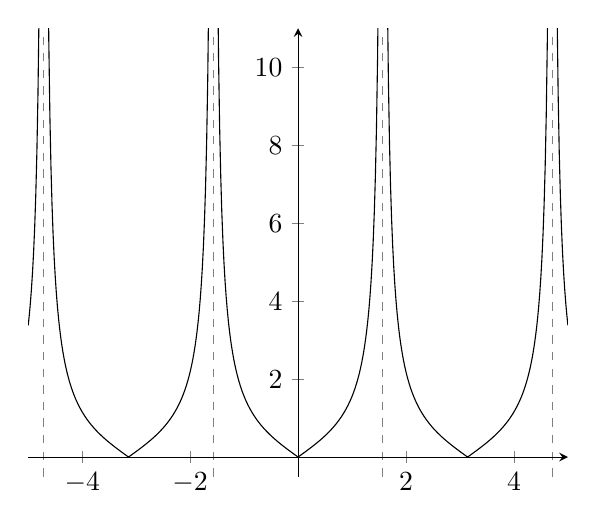
\begin{tikzpicture}
						\begin{axis} [
							axis lines = center,
							axis on top=true,
							ymax = 11, ymin = -.5
						]
							\addplot [domain=-5:5,samples=500] {abs(tan(deg(x)))};
							\draw [dashed, color=black!50] (axis cs:pi/2,-.5) -- (axis cs:pi/2,11);
							\draw [dashed, color=black!50] (axis cs:3*pi/2,-.5) -- (axis cs:3*pi/2,11);
							\draw [dashed, color=black!50] (axis cs:-pi/2,-.5) -- (axis cs:-pi/2,11);
							\draw [dashed, color=black!50] (axis cs:-3*pi/2,-.5) -- (axis cs:-3*pi/2,11);
						\end{axis}
					\end{tikzpicture}
				}
			\end{center}
		\end{minipage}
		\begin{minipage}{0.49\linewidth}
			\begin{center}
				\resizebox{\linewidth}{!}{
					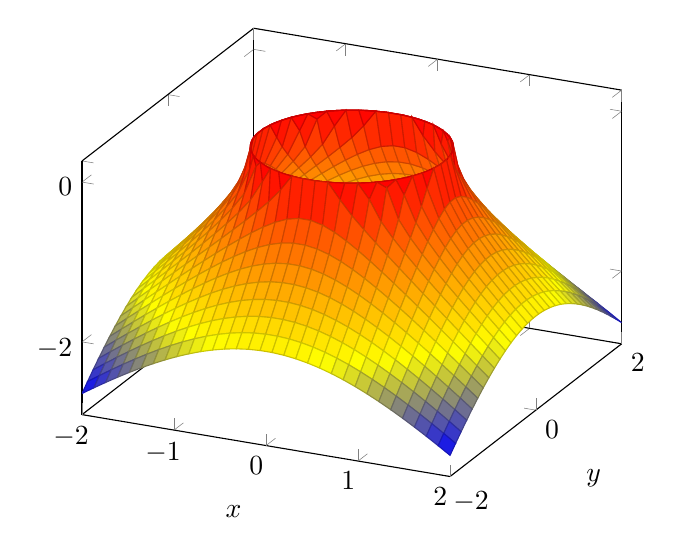
\begin{tikzpicture}
						% Thanks to Symbol 1 from https://tex.stackexchange.com/a/543874/206062
						\pgfmathdeclarefunction{volcano_z}{2}{%
							\pgfmathsetmacro\radsq{#1^2 + #2^2}% \radsq is radius^2 in FPU notation
							\pgfmathfloattofixed{\radsq}\let\radsqsafe=\pgfmathresult % in safe notation
							\ifdim\radsqsafe pt > 1pt\relax
								\pgfmathparse{-sqrt(\radsq-1)}%
							\else\ifdim\radsqsafe pt > 0.25pt\relax
								\pgfmathparse{+0}%
							\else % \radsq pt <= 0.25
								\pgfmathparse{NaN}%
							\fi\fi
						}
						\pgfmathdeclarefunction{volcano_x}{2}{%
							\pgfmathsetmacro\radsq{#1^2 + #2^2}% \radsq is radius^2 in FPU notation
							\pgfmathfloattofixed{\radsq}\let\radsqsafe=\pgfmathresult % in safe notation
							\ifdim\radsqsafe pt > 1pt\relax
								\pgfmathparse{#1}%
							\else\ifdim\radsqsafe pt > 0.25pt\relax
								\pgfmathparse{#1/sqrt(\radsq)}%
							\else % \radsq pt <= 0.25
								\pgfmathparse{NaN}%
							\fi\fi
						}
						\begin{axis}[
							xlabel=$x$, ylabel=$y$,
							]
							\addplot3[surf,domain =-2:2,unbounded coords=jump,samples=32]
								({volcano_x(x,y)}, {volcano_x(y,x)}, {volcano_z(x,y)});
						\end{axis}
					\end{tikzpicture}
				}
			\end{center}
		\end{minipage}
	\end{solution}
\end{exercise}
\begin{exercise}
	\label{ex:uniq_max_min_abs}
	Formulare e dimostrare l'unicità del massimo/minimo assoluto.
	\begin{note}
		Notare che è richiesta l'unicità del \textbf{massimo/minimo assoluto}, non dei punti di massimo/minimo. Si ricorda l'\fullref{obs:inf_pti_max_min_abs}.
	\end{note}
	\begin{solution}
		Per definizione, $x = \max X$ se $x = \sup X$ e $x \in X$. Se poi $x = \sup X$, allora $x$ è per definizione il più piccolo dei maggioranti di $X$.\\
		Il $\sup$ di un insieme è unico, si dimostra per assurdo:
		\begin{proof}
			\renewcommand\qedsymbol{$\square$} % To restore the default empty square for this proof environment
			Dati $A \subseteq \R$ e $B \subseteq A$, si supponga esistano $M_1, M_2 \in A$ con $M_1 \neq M_2$, due $\sup$ diversi di $B$. Applicando la definizione di maggiorante:
			\[\forall x \in B,\; x \leq M_1 \qquad \text{e} \qquad \forall x \in B,\; x \leq M_2\]
			Si può ora supporre che sia $M_1 > M_2$ senza perdere generalità, però questo significa che $M_1$ non sia $\sup$, (non è il più piccolo dei maggioranti), negando l'ipotesi - \textit{Assurdo}
		\end{proof}
		Per come è definito dunque, anche il $\max$ sarà unico, da cui la tesi.
	\end{solution}
\end{exercise}
\begin{exercise}
	\label{ex:max_min_lib_funz_in_R}
	In questa sezione compaiono esclusivamente funzioni a valori in $\R$. Perché?
	\begin{solution}
		Perché si stanno considerando i valori assunti dalla $f$ come punti nello spazio (nella retta reale, essendo in $\R$) e non esistono necessariamente relazioni d'ordine in altri insiemi. Non è possibile ad esempio stabilire se un punto punto sia "maggiore o minore" di un altro in $\R^2$ o in $\C$.
	\end{solution}
\end{exercise}

\subsection{Condizioni Necessarie}
\begin{proposition}
	\label{prop:f_deriv_pto_estr_deriv_direz_nulla}
	Siano $A \subseteq \R^n$, $x_0 \in \circdot{A}$, $f: A \to \R$ e $v \in \R^n \setminus {0}$, allora
	\[
		\left.
			\begin{array}{c}
				f \text{ \textbf{derivabile} in } x_0 \text{ lungo } v\\
				x_0 \text{ punto \textbf{di estremo} per } f
			\end{array}
		\right\}
		\implies
		D_vf(x_0) = 0
	\]
	\begin{proof}
		Se $x_0$ è di estremo per $f$, allora, scelto un opportuno $\delta > 0 \in \R$, $x_0$ è di estremo anche per la funzione
		\[\funcdef{\varphi}{\intervalopen{-\delta}{\delta}}{\R}{t}{f(x_0 + tv)}\]
		La $\varphi$ è una funzione reale di variabile reale e derivabile in $0$ perché $f$ è derivabile per ipotesi. Ciò significa che è possibile applicare alla $\varphi$ il \textit{Teorema di Fermat} di Analisi 1, avendo la garanzia che in un punto estremante di questa funzione sia $\varphi'(x_0) = 0$.\\
		Applicando ora la definizione di derivata di Analisi 1 si ottiene:
		\[
			\varphi'(t) = \lim\limits_{h \to 0} \frac{\varphi(t + h) - \varphi(t)}{h}
		\]
		Se si calcola la derivata di $\varphi$ nel punto $0$ ($\varphi(0) = f(x_0)$, con $x_0$ estremante per ipotesi) si ottiene:
		\begin{align*}
			0 &= \varphi'(0)\\
			&= \lim\limits_{h \to 0} \frac{\varphi(h) - \varphi(0)}{h}
			\shortintertext{Ma, essendo $\varphi(h) = f(x_0 + hv)$ e $\varphi(0) = f(x_0)$}
			&= \lim\limits_{h \to 0} \frac{f(x_0 + hv) - f(x_0)}{h} \tageq\label{eq:estr_f_allora_Dvf_0}
		\end{align*}
		La \cref{eq:estr_f_allora_Dvf_0} non è altro che la \fullref{def:deriv_direz} di $f$ in $x_0$ lungo il vettore $v$, dunque si è giunti alla tesi.
	\end{proof}
\end{proposition}
\begin{theorem}[di Fermat]
	\label{teo:fermat}
	Siano $A \subseteq \R^n$, $x_0 \in \circdot{A}$ e $f: A \to \R$, allora
	\[
		\left.
			\begin{array}{c}
				f \text{ \textbf{Differenziabile} in } x_0\\
				x_0 \text{ punto \textbf{di estremo} per } f
			\end{array}
		\right\}
		\implies
		\nabla f(x_0) = 0
	\]
	\begin{proof}
		Dalla \fullref{prop:se_diff_deriv_dir}, si sa che, se $f$ è differenziabile, allora
		\[\forall v \in \R^n \setminus {0} \quad D_vf(x_0) = Df(x_0) v\]
		Quindi $\forall v \in \R^n \setminus {0}$ si può applicare la \fullref{prop:f_deriv_pto_estr_deriv_direz_nulla}. Visto poi che la $f$ è a valori in $\R^1$, da \fullref{obs:matr_deriv_tot} si sa che $Df(x_0) = \nabla f(x_0)$, dunque la tesi:
		\[0 = D_vf(x_0) = Df(x_0) = \nabla f(x_0)\]
	\end{proof}
\end{theorem}
\begin{definition}[Punto Stazionario]
	\label{def:pto_staz}
	Siano $A \subseteq \R^n$, $x_0 \in \circdot{A}$ e $f: A \to \R$
	\[
		x_0 \text{ \textbf{Punto Stazionario} per } f
		\quad \bydef \quad
		\begin{cases}
			\begin{array}{c}
				f \text{ \textbf{Differenziabile} in } x_0\\[-1ex]
				e\\[-1ex]
				\nabla f(x_0) = 0
			\end{array}
		\end{cases}
	\]
	\begin{note}
		Nella definizione si usa $\nabla f$ in luogo di $Df$ perché la $f$ è a valori in $\R$, dunque come visto in \fullref{obs:matr_deriv_tot} $Df$ è $\in \mat(1 \times n)$, cioè $Df = \nabla f$ per definizione di gradiente.
	\end{note}
\end{definition}
\begin{observation}
	Grazie al \fullref{coro:se_diff_deriv_parz}, se $f$ \textbf{Differenziabile} in $x_0$, per verificare che $\nabla f(x_0) = 0$, basta verificare che le \textbf{Derivate Parziali} siano tutte pari a $0$.
\end{observation}
\begin{exercise}
	Esibire un esempio di funzione che ammetta un punto stazionario non di estremo, cioè la tesi del \fullref{teo:fermat}, ma che non verifichi le ipotesi.
	\begin{solution}
		$f(x) = x^3$ ha un punto stazionario in $x=0$, ma sicuramente non è minimo o massimo.
	\end{solution}
\end{exercise}
\begin{exercise}
	Esibire una funzione che ammetta un punto di estremo non stazionario
	\begin{solution}
		In $x = 3$ la funzione
		\[\funcdef{f}{\intervalopcl{0}{3}}{\R}{x}{\sqrt{x}}\]
		è differenziabile, ma $\nabla f(3) = \frac{1}{2\sqrt{3}} \neq 0$, dunque non è stazionario.
	\end{solution}
\end{exercise}

\vspace*{\baselineskip}
Nelle seguenti proposizioni verranno usate la \fullref{def:differenz_second} e la notazione introdotta in Appendice nella \fullref{sect:for_quadr}. Si ricorda che $D^2f(x_0) = H_f(x_0)$ da \fullref{def:hessiana}.
\begin{proposition}
	\label{prop:pto_max_D2f_semdef_neg}
	Siano $A \subseteq \R^n$, $x_0 \in \circdot{A}$ e $f: A \to \R$
	\[
		\left.
			\begin{array}{c}
				f \text{ \textbf{Differenziabile 2 volte} in } x_0\\
				x_0 \text{ punto \textbf{di massimo} per } f
			\end{array}
		\right\}
		\implies
		\begin{cases}
			\nabla f(x_0) = 0\\
			D^2f(x_0) = H_f(x_0) \text{ \textbf{Semidefinita Negativa}}
		\end{cases}
	\]
	\begin{proof}
		Essendo $x_0$ punto di massimo per ipotesi, è certo che, per un $h \in \R^n$ in intorno di $0$:
		\begin{equation}
			\label{eq:pto_max_hess_semdef_neg_diff}
			f(x_0 + h) - f(x_0) \leq 0
		\end{equation}
		Posto $x = x_0 + h$, si ha che $h = x - x_0$, dunque dalla \fullref{prop:svil_tay_2_peano} si ha:
		\begin{align*}
			f(x) &= f(x_0) + Df(x_0)h + \frac{1}{2} h^T D^2f(x_0) h + o\left( \norm{h}^2 \right)\\
			f(x) - f(x_0) &= \nabla f(x_0)(x - x_0) + \frac{1}{2} (x - x_0)^T D^2f(x_0)(x - x_0) + o\left( \norm{(x - x_0)}^2 \right)
			\shortintertext{Essendo però $\nabla f(x_0) = 0$ per ipotesi}
			f(x) - f(x_0) &= \frac{1}{2} (x - x_0)^T D^2f(x_0)(x - x_0) + o\left( \norm{(x - x_0)}^2 \right)
		\end{align*}
		Il termine di sinistra non è altro che il primo termine della \cref{eq:pto_max_hess_semdef_neg_diff}, dunque
		\begin{align*}
			\frac{1}{2} (x - x_0)^T D^2f(x_0)(x - x_0) + o\left( \norm{(x - x_0)}^2 \right) &\leq 0
			\shortintertext{L'\textit{o piccolo} può essere ignorato in quanto, per definizione, tende a zero più velocemente del resto della funzione}
			\frac{1}{2} (x - x_0)^T D^2f(x_0)(x - x_0) &\leq 0\\
			(x - x_0)^T D^2f(x_0)(x - x_0) &\leq 0
		\end{align*}
		Da cui, per la \fullref{def:def_semdef_pos_neg}, deriva che la $D^2f(z_0)$ è Semidefinita Negativa.
	\end{proof}
\end{proposition}
\begin{proposition}
	Siano $A \subseteq \R^n$, $x_0 \in \circdot{A}$ e $f: A \to \R$
	\[
		\left.
			\begin{array}{c}
				f \text{ \textbf{Differenziabile 2 volte} in } x_0\\
				x_0 \text{ punto \textbf{di minimo} per } f
			\end{array}
		\right\}
		\implies
		\begin{cases}
			\nabla f(x_0) = 0\\
			D^2f(x_0) = H_f(x_0) \text{ \textbf{Semidefinita Positiva}}
		\end{cases}
	\]
	\begin{proof}
		Applicare la \fullref{prop:pto_max_D2f_semdef_neg} a $-f$
	\end{proof}
\end{proposition}
\begin{exercise}
	Esibire una funzione soddisfacente alla tesi della \fullref{prop:pto_max_D2f_semdef_neg}, ma non alle ipotesi.
\end{exercise}

\subsection{Condizioni Sufficienti}
\begin{proposition}
	Siano $A \subseteq \R^n$, $x_0 \in \circdot{A}$ e $f: A \to \R$
	\[
		\left.
			\begin{array}{c}
				f \text{ \textbf{Differenziabile 2 volte} in } x_0\\
				\nabla f(x_0) = 0\\
				D^2f(x_0) = H_f(x_0) \text{ \textbf{Definita Negativa}}
			\end{array}
		\right\}
		\implies
		x_0 \text{ \textbf{punto di Massimo Locale} per } f
	\]
	\begin{proof}
		Per un $h \in \R^n$ in intorno di $0$ e posto $x = x_0 + h$, sfruttando la \fullref{prop:svil_tay_2_peano} si ha:
		\begin{align*}
			f(x_0 + h) &= f(x_0) + Df(x_0)h + \frac{1}{2} h^T D^2f(x_0) h + o\left( \norm{h}^2 \right)\\
			f(x_0 + h) - f(x_0) &= \nabla f(x_0)h + \frac{1}{2} h^T D^2f(x_0) h + o\left( \norm{h}^2 \right)
			\shortintertext{Essendo però $\nabla f(x_0) = 0$ per ipotesi}
			&= \frac{1}{2} \underbrace{h^T D^2f(x_0) h}_{\text{(1)}} + o\left( \norm{h}^2 \right)
			\shortintertext{La (1) è una forma quadratica del tipo $q(h)$ con $D^2f(x_0)$ definita negativa per ipotesi. Dunque, applicando il \fullref{coro:form_quadr_def_neg_q_leq_-m} è possibile minorare con}
			&\leq -\frac{1}{2} m \norm{h}^2 + o(\norm{h}^2)\\
			&= \underbrace{\left( -\frac{1}{2} m + o(1) \right)}_{\leq 0} \underbrace{\norm{h}^2}_{\geq 0}\\
			&\leq 0
		\end{align*}
	\end{proof}
\end{proposition}
\begin{corollary}
	Siano $A \subseteq \R^n$, $x_0 \in \circdot{A}$ e $f: A \to \R$
	\[
		\left.
			\begin{array}{c}
				f \text{ \textbf{Differenziabile 2 volte} in } x_0\\
				\nabla f(x_0) = 0\\
				D^2f(x_0) = H_f(x_0) \text{ \textbf{Definita Positiva}}
			\end{array}
		\right\}
		\implies
		x_0 \text{ \textbf{punto di Minimo Locale} per } f
	\]
	\begin{proof}
		Analoga alla precedente applicando \fullref{prop:form_quadr_def_pos_q_geq_m}.
	\end{proof}
\end{corollary}
\begin{exercise}
	Applicare, quando possibile, le proposizioni di questa sezione e della precdente alle seguenti funzioni, tutte definite su $\R^2$\\
	\begin{minipage}{0.49\linewidth}
		\begin{align*}
			f(x,y) &= x^2 + y^2\\
			f(x,y) &= -x^2 + y^2\\
			f(x,y) &= x^4 + y^4\\
			f(x,y) &= -x^4 - y^4\\
			f(x,y) &= \abs{x} + y^2
		\end{align*}
	\end{minipage}
	\begin{minipage}{0.49\linewidth}
		\begin{align*}
			f(x,y) &= x^2 - y^2\\
			f(x,y) &= -x^2 - y^2\\
			f(x,y) &= x^4 + y^3\\
			f(x,y) &= x^2 - y^2\\
			f(x,y) &= -x \abs{x} - y^3
		\end{align*}
	\end{minipage}
	% TODO solution
\end{exercise}

\newpage
\section{Massimi e Minimi Vincolati}
Spesso la ricerca di punti di massimo o minimo di una funzione $f:A \to \R$ con $A \subseteq \R^n$ deve essere ristretta ad un sottoinsieme $B \subset A$ a causa di eventuali vincoli che le variabili indipendenti devono soddisfare. L'insieme $B$ può essere generalmente descritto da una funzione \textbf{Vincolo} $\varphi: A \to \R^p$, nel senso che $B = \brackets{x \in A: \varphi(x) \leq 0}$\\
Questo problema è usualmente abbreviato in:
\[\max\limits_{\varphi \leq 0} f \qquad \text{oppure} \qquad \min\limits_{\varphi \leq 0} f\]
e può essere diviso in due passi:
\begin{enumerate}
	\item ricerca dei punti di estremo di $f$ interni a $B$ (problema già affrontato con gli estremi liberi)
	\item ricerca dei punti di estremo di $f$ sul bordo di $B$ (si andrà a studiare ora)
\end{enumerate}
Sotto opportune condizioni per $\varphi$, infatti:
\[\circdot{B} = \brackets{x\in A: \varphi(x) < 0} \qquad \text{e} \qquad \partial B\brackets{x\in A: \varphi(x) = 0}\]
Dunque si possono individuare gli estremi in due insiemi diversi in due passaggi separati con modalità diverse.
\begin{note}
	Quanto detto è in accordo con la \fullref{def:max_min}, che infatti non esclude il caso di punti di estremo vincolati alla frontiera di un insieme.
\end{note}
\begin{theorem}[dei Moltiplicatori di Lagrange]
	\label{teo:molt_lagr_gen}
	Sia $A \subseteq \R^n$ un \textbf{Aperto} e siano
	\begin{itemize}[noitemsep]
		\item $f: A \to \R$
		\item $\varphi: A \to \R^p$ con $p < n$ e $\varphi^{-1}(0) \subset A$
	\end{itemize}
	\begin{note}
		$\varphi$, vincolo, è funzione di $p$ funzioni $\varphi_i$ per $i = 1,\:\dotsc\:,p$.
	\end{note}
	due funzioni $\in \cntclass{1}$.
	Se:
	\begin{itemize}[noitemsep]
		\item $x_0$ è un punto di \textbf{estremo relativo} per $f$ \textbf{vincolata} a $\varphi = 0$
		\item $\rank \bigl( D\varphi(x_0) \bigr) = p$, cioè $D\varphi(x_0)$ ha \textbf{rango} $p$
	\end{itemize}
	\begin{note}
		\hypertarget{note:teo_molt_lagr_gen}{}
		Essendo $\varphi$ funzione di funzioni, $D\varphi(x_0)$ è una matrice costituita:
		\[
			D\varphi(x_0) =
			\begin{bmatrix}
				\partial_{x_1} \varphi_1 & \partial_{x_2} \varphi_1 & \cdots & \partial_{x_n} \varphi_1\\
				\partial_{x_1} \varphi_2 & \partial_{x_2} \varphi_2 & \cdots & \partial_{x_n} \varphi_2\\
				\vdots & \vdots & \ddots & \vdots\\
				\partial_{x_1} \varphi_p & \partial_{x_2} \varphi_p & \cdots & \partial_{x_n} \varphi_p
			\end{bmatrix}
		\]
		In cui ogni riga è il gradiente della $i$\textit{-esima} funzione, $\nabla \varphi_i$.\\
		Richiedere $\rank \bigl( D\varphi(x_0) \bigr) = p$ significa imporre che i $p$ vincoli siano tutti linearmente indipendenti, cioè che siano tutti "indicativi" (è inutile avere 2 vincoli uguali).\\
		Inoltre la condizione garantisce che, per ogni vincolo, almeno una delle derivate parziali sia non nulla. Se infatti tutte le derivate parziali di una $\varphi_i$ fossero nulle, il rango della matrice non sarebbe più $p$.
	\end{note}
	Allora esistono $p$ numeri reali $\lambda_1,\; \lambda_2,\:\dotsc\:\lambda_p$ tali che
	\begin{equation}
		\label{eq:eqiv_nabl_molt_lagr}
		\nabla f(x_0) = \sum\limits_{i = 1}^{p} \lambda_i \nabla \varphi_i (x_0)
	\end{equation}
	Gli scalari $\lambda_i$ sono comunemenete chiamati \textbf{Moltiplicatori di Lagrange} e i $\nabla \varphi_i (x_0)$ sono i gradienti delle $p$ funzioni vincolo che compongono $\varphi$.\\
	Cioè la combinazione lineare di tutti i $\nabla \varphi_i$ corrisponde a $\nabla f$.
	\begin{note}
		La combinazione lineare, per definzione, è somma delle componenti ognuna con un appropriato coefficiente $\lambda_i$
	\end{note}
	\begin{proof}
		Omessa. Verrà svolta in seguito per il caso $n = 2, m = 1$ in \fullref{teo:molt_lagr_n2_m1}.
	\end{proof}
\end{theorem}
\begin{observation}
	Il \fullref{teo:molt_lagr_gen} può essere visto come una generalizzazione del \fullref{teo:fermat} nella ricerca degli estremi di funzioni vincolate.
\end{observation}
\begin{observation}[Spiegazione Concetto]~
	\label{obs:concetto_teo_molt_lagr_gen}
	\begin{center}
		% Thanks to https://it.wikipedia.org/wiki/Metodo_dei_moltiplicatori_di_Lagrange
		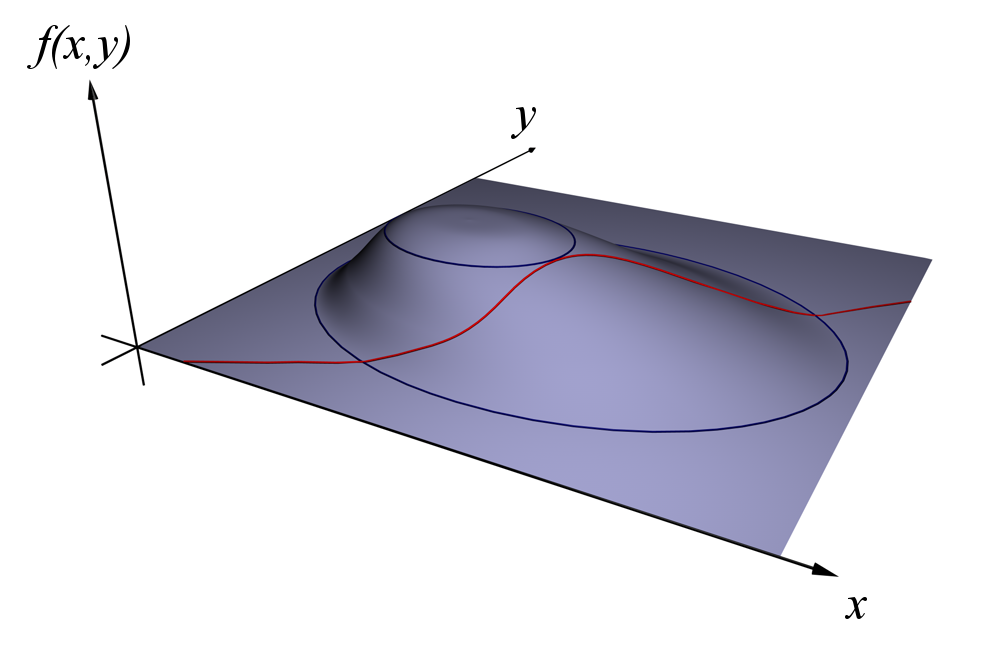
\includegraphics[width=.49\linewidth]{3d-lagrange-multipliers}
		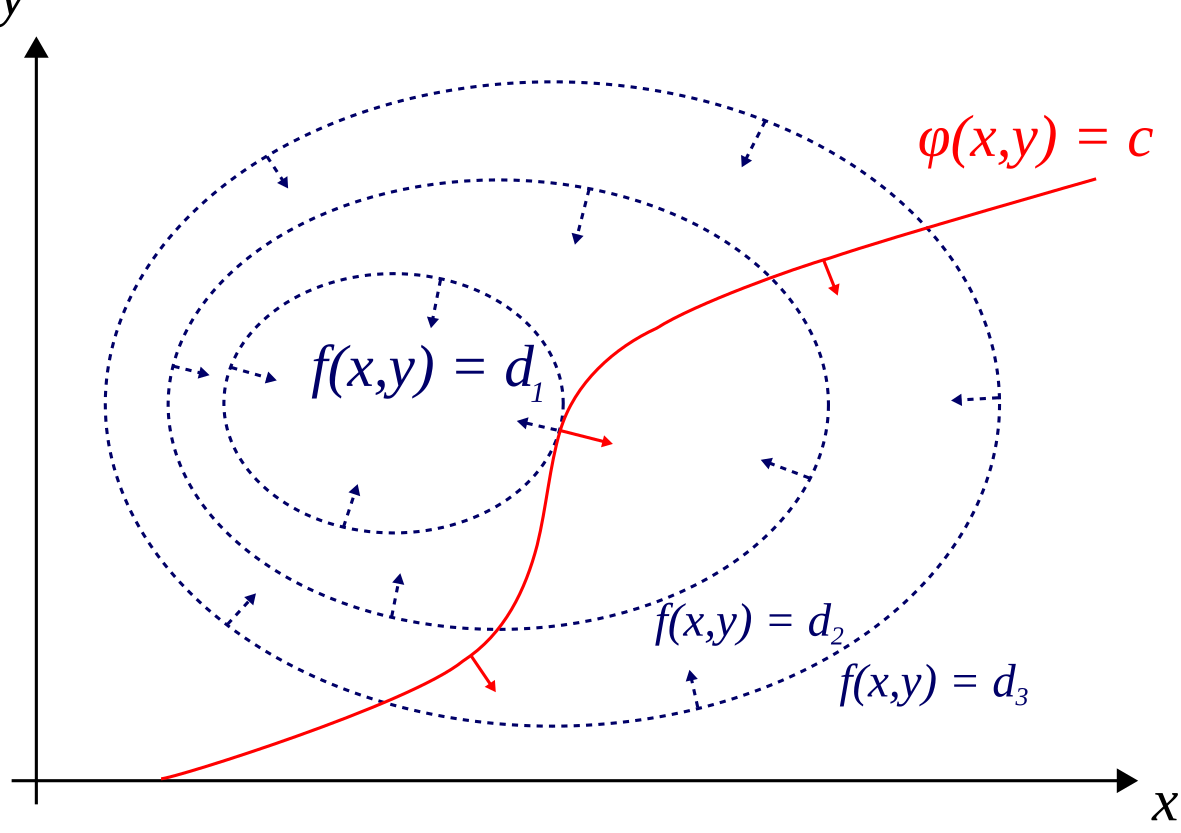
\includegraphics[width=.49\linewidth]{2d-lagrange-multipliers}
	\end{center}
	Data una certa $f: A \mapsto \R$, le sue \fullref{def:curv_liv} sono i luoghi dei punti soddisfacenti l'equazione $f(x) = d$, con $x \in A$ e $d \in \R$ generico. Si sta ora cercando di massimizzare la $f$ \textit{rispettando il vincolo} $\varphi(x)$, o, detto in modo diverso, di massimizzarla \textit{lungo il vincolo} $\varphi(x)$.\\
	Le Curve di Livello di $\varphi$ saranno a loro volta luoghi dei punti tali per cui $\varphi(\xi) = c$, con $\xi \in A$ e $c \in \R$ generico.

	Le Curve di Livello di $f$ e $\varphi$ sono, in generale, distinte, dunque le C.D.L. di $f$ possono benissimo intersecare una qualsiasi $\varphi(\xi) = c$. Per definizione di C.D.L., muovendosi lungo una C.D.L. di $\varphi$, il valore assunto dalla $\varphi$ rimarrà costante, mentre il valore di $f$ può variare, come appena detto. Nel caso però in cui $\varphi(\xi) = c$ è \textbf{tangente} ad una C.D.L. di $f$, allora spostandosi lungo la C.D.L. di $\varphi$, rimarrà costante anche la $f$.\\
	Come visto in \fullref{def:pto_staz}, $f$ è costante quando $\nabla f(x_0) = 0$ e, come si vedrà in \fullref{prop:curv_liv_perp_grad} la C.D.L è $\perp \nabla f$. Quanto detto fino ad ora però permette di aggiungere che la $f$ sia costante anche quando $\nabla f \parallel \nabla \varphi$, cioè quando $\nabla f$ è \textbf{Combinazione Lineare} delle $\nabla \varphi_i$.
\end{observation}
\begin{observation}
	Si noti che anche nel caso $n = 2$, $p = 1$ nella \cref{eq:eqiv_nabl_molt_lagr} non sarebbe coretto spostare $\lambda$ all'altro termine:
	\[\lambda \nabla f(x_0, y_0) = \nabla \varphi (x_0, y_0) \tag{\textbf{Errato!}}\]
	Per quanto questa possa sembrare una semplice divisione per uno scalare, in realtà sarebbe una possibile svista. Il valore di $\nabla f(x_0,y_0)$ infatti non è noto a prescindere e, se fosse nullo, questa scrittura sarebbe in contrasto con l'ipotesi $\nabla \varphi(x_0,y_0) \neq 0$
\end{observation}
\begin{example}
	\label{ex:max_min_vinc_n2_p1}
	Nel caso in cui $A \subseteq \R^2$, cioè il caso più comune, si hanno
	\begin{itemize}[noitemsep]
		\item $f: A \to \R$
		\item $\varphi: A \to \R^p = \R^1$
	\end{itemize}
	Perché $p < 2$, dunque sicuramente $p = 1$.
\end{example}
\cbstart
\begin{definition}[Funzione Lagrangiana] % Come definita su https://en.wikipedia.org/wiki/Lagrange_multiplier
	\label{def:funz_lagr}
	Sia $A \subseteq \R^n$ un \textbf{Aperto}, $x \in A$, $\lambda \in \R^p$ con $p < n$, allora si definisce la
	\[\mathcal{L}(x, \lambda) = f(x) - \lambda \varphi(x)\]
	cioè, "espandendo" le variabili per chiarezza
	\[\mathcal{L}(x_1,\:\dotsc\:,x_n, \lambda_1,\:\dotsc\:,\lambda_p) = f(x_1,\:\dotsc\:,x_n) - \sum\limits_{i = 1}^{p} \lambda_i \nabla \varphi_i (x_1,\:\dotsc\:,x_n)\]
	$\mathcal{L}$ è una funzione ausiliaria, nota come \textbf{Funzione Lagrangiana}, che lega la $f$ ed il vincolo $\varphi$.

	\noindent I punti stazionari \textbf{Vincolati} della $f$ sono i punti stazionari \textbf{Liberi} della Lagrangiana.
\end{definition}
\cbend
\begin{observation}
	\label{obs:sist_eqiv_lagr}
	Mediante il \fullref{teo:molt_lagr_gen}, la ricerca di punti di estremo per $f$ vincolati a $\varphi = 0$ viene dunque ricondotta alla risoluzione del sistema:
	\begin{equation}
		\label{eq:teo_molt_lagr_gen_sist_varphi}
		\begin{cases}
			\nabla f(x_0) = \sum\limits_{i = 1}^{p} \lambda_i \nabla \varphi_i (x_0)\\
			\varphi(x_0) = 0
		\end{cases}
	\end{equation}
\end{observation}
\begin{exercise}
	Verificare che, con la notazione del \fullref{teo:molt_lagr_gen}, il sistema \cref{eq:teo_molt_lagr_gen_sist_varphi} è un sistema di $n + p$ equazioni in $n + p$ incognite.
	\begin{solution}
		Da \fullref{def:funz_lagr}, calcolando $\nabla \mathcal{L}(x, \lambda) = 0$ si ottiene
		\[
			\nabla_{x_1,\:\dotsc\:,x_n, \lambda_1,\:\dotsc\:,\lambda_p} \mathcal{L}(x_1,\:\dotsc\:, x_n, \lambda_1,\:\dotsc\:,\lambda_p)=0
			\iff
			\begin{cases}
				\nabla f(x) - \sum\limits_{i=1}^{p} {\lambda_i \: \nabla \varphi_i (x)} = 0\\
				\varphi_1(x) = \cdots = \varphi_p(x) = 0
			\end{cases}
		\]
		Con la seconda condizione dovuta all'ipotesi del \fullref{teo:molt_lagr_gen} per cui il vincolo è $\varphi = 0$.\\
		Essendo la \cref{eq:teo_molt_lagr_gen_sist_varphi} un'equazione in $n + p$ variabili, anche il sistema in oggetto non può che essere a $n + p$ equazioni in $n + p$ incognite.
	\end{solution}
\end{exercise}
\begin{example}
	\label{ex:molt_lagr_sist_equiv}
	In $A \subseteq \R^2$, dato un problema del tipo $\max\limits_{\varphi(x,y)=0} f$, cioè la ricerca del massimo di $f$ sul vincolo $\varphi(x,y)=0$, come detto in \fullref{obs:sist_eqiv_lagr}, ci si può ricondurre ad un sistema del tipo
	\[
		\begin{cases}
			\nabla f(x_0,y_0) = \lambda \nabla \varphi(x_0,y_0)\\
			\varphi(x_0,y_0)=0
		\end{cases}
		=
		\begin{cases}
			\partial_xf(x_0,y_0) = \lambda \partial_x \varphi(x_0,y_0)\\
			\partial_yf(x_0,y_0) = \lambda \partial_y\varphi(x_0,y_0)\\
			\varphi(x_0,y_0)=0
		\end{cases}
	\]
	a 3 equazioni in 3 incognite: $(x, y, \lambda)$.
	\begin{solution}~
		\begin{note}
			Questa soluzione è molto simile alla dimostrazione del \fullref{teo:molt_lagr_n2_m1}.
		\end{note}
		Per ipotesi del \fullref{teo:molt_lagr_gen}, $\rank \bigl( D\varphi(x_0, y_0) \bigr) = p = 1$, dunque come da \hyperlink{note:teo_molt_lagr_gen}{nota alle ipotesi del \fullref*{teo:molt_lagr_gen}}:
		\[
			\begin{bmatrix}
				\partial_x\varphi(x_0,y_0) & \partial_y\varphi(x_0,y_0)
			\end{bmatrix}
			\neq
			\begin{bmatrix}
				0 & 0
			\end{bmatrix}
		\]
		Ciò vuol dire che, sicuramente, $\partial_x \varphi(x_0,y_0) \neq 0$ oppure $\partial_y \varphi(x_0,y_0) \neq 0$.

		\vspace*{\baselineskip}
		Supponendo $\partial_y \varphi(x_0,y_0) \neq 0$ e sapendo che per ipotesi $\varphi(x,y) = 0$, si applica il \fullref{teo:funz_impl}
		\begin{note}
			Verifica ipotesi:
			\begin{enumerate}
				\item $A \subseteq \R \times \R$ aperto per ipotesi \fullref{teo:molt_lagr_gen}
				\item $f \in \cntclass{1}$ per ipotesi \fullref{teo:molt_lagr_gen}, quindi sicuramente continua
				\item $(x_0, y_0) \in A$ e $\varphi(x_0, y_0) = 0$ per ipotesi \fullref{teo:molt_lagr_gen}
				\item $f \in \cntclass{1}$ per ipotesi \fullref{teo:molt_lagr_gen}, quindi $D_y f$ esiste continua in $(x_0, y_0)$
				\item $D_yf(x_0, y_0)$ ammette inversa perché è stato ipotizzato $\partial_y \varphi(x_0,y_0) \neq 0$ poco sopra
			\end{enumerate}
		\end{note}
		Grazie al \fullref{teo:funz_impl} si ha che esistono degli intorni $\mathcal{X}$ di $x_0$ e $\mathcal{Y}$ di $y_0$ e, per $x \in \mathcal{X}$ e $y \in \mathcal{Y}$, esiste la
		\[g: \mathcal{X} \to \mathcal{Y} \quad \text{tale che} \quad \varphi(x,y) = 0 \iff y = g(x)\]
		Avendo la certezza dell'esistenza della $g$, è possibile concludere che:
		\[
			(x_0,y_0) \text{ di Estremo per } f(x,y) \text{ ristretta a } \mathcal{X} \times \mathcal{Y}
			\quad \iff \quad
			x_0 \text{ di Estremo per } f\bigl( x, g(x) \bigr)
		\]
		Dunque, per il \fullref{teo:fermat}, è garantito che $\nabla f\bigl( x_0, g(x_0) \bigr) = 0$. Calcolando ora $\nabla f\bigl( x_0, g(x_0) \bigr)$ grazie alla \fullref{prop:deriv_funz_comp}
		\begin{align*}
			0
			&=	\partial_x f\bigl( x_0, g(x_0) \bigr) +
				\partial_y f\bigl( x_0, g(x_0) \bigr) \cdot
				g'(x_0)\\
			&=	\partial_x f\bigl( x_0, g(x_0) \bigr) +
				\partial_y f\bigl( x_0, g(x_0) \bigr) \cdot
				\left(
					-
					\frac{
						\partial_x g(x_0,g(x_0))
					}{
						\partial_y g(x_0,g(x_0))
					}
				\right)\\
			&=	\partial_x f\bigl( x_0, g(x_0) \bigr) \cdot \partial_y g(x_0,g(x_0)) -
				\partial_y f\bigl( x_0, g(x_0) \bigr) \cdot \partial_x g(x_0,g(x_0))
			\shortintertext{Che può essere rappresentato in forma compatta come il $\det$ di una matrice $\mat (2 \times 2)$}
			&=	\det \left(
				\begin{matrix}
					\partial_xf(x_0,y_0) & \partial_yf(x_0,y_0)\\
					\partial_xg(x_0,y_0) & \partial_yg(x_0,y_0)
				\end{matrix}
				\right)
		\end{align*}
		Prendendo il primo e l'ultimo elemento del treno di uguaglianze si ha che $\det = 0$, dunque, dalle nozioni di Algebra, si sa che questo implica il parallelismo tra i vettori della matrice. Essendo la $g$ e la $\varphi$ legate implicitamente, è possibile concludere che:
		\[\exists \lambda \in \R: \nabla f(x_0,y_0) = \lambda \nabla \varphi(x_0,y_0)\]
	\end{solution}
\end{example}

\newpage
\section{Il Caso \texorpdfstring{$n=2,\,m=1$}{n=2, m=1}}
Quanto esposto in questa sezione può essere esteso al caso $n > 2$ a patto di notevoli cambiamenti nella terminologia geometrica.
\begin{definition}[Grafico]
	Siano $A \subseteq \R^2$ e $f: A \to \R$. La superficie di equazione
	\[z = f(x,y)\]
	è il \textbf{Grafico} di $f$
\end{definition}
\begin{definition}[Curva di Livello]
	\label{def:curv_liv}
	Siano $A \subseteq \R^2$, $f: A \to \R$ e $c \in \R$. L'insieme
	\[f^{-1}(c) = \brackets{(x,y) \in A:\; f(x,y) = c}\]
	è la \textbf{Curva di Livello} $\boldsymbol{c}$ di $f$
\end{definition}
\begin{definition}[Piano Tangente]
	Siano $A \subseteq \R^2$, $f: A \to \R$, $f$ \textbf{Differenziabile} in $(x_0, y_0) \in \circdot{A}$. Allora
	\begin{align*}
		z &=
		f(x_0, y_0) +
		\nabla f(x_0, y_0) \cdot
		\begin{bmatrix}
			x - x_0\\
			y - y_0
		\end{bmatrix}\\
		&=
		f(x_0, y_0) +
		\begin{bmatrix}
			\partial_xf(x_0,y_0) & \partial_yf(x_0,y_0)
		\end{bmatrix}
		\cdot
		\begin{bmatrix}
			x - x_0\\
			y - y_0
		\end{bmatrix}\\
		&= f(x_0, y_0) + \partial_xf(x_0,y_0) \; (x - x_0) + \partial_yf(x_0,y_0) \; (y - y_0)
	\end{align*}
	è il \textbf{Piano Tangente} alla superficie $x = f(x,y)$ in $(x_0, y_0)$
	\begin{note}
		Non c'è ovviamente alcuna differenza tra le tre equazioni sopra.
	\end{note}
\end{definition}
\begin{observation}
	Il \textbf{Grafico} di $f$ è un \textbf{sottoinsieme} di $\R^3$.\\
	Il \textbf{Gradiente} e le \textbf{Curve di Livello} "vivono" nell'insieme partenza $A \subseteq \R^2$, come si può vedere dal seguente grafico: il gradiente non esce dall'insieme di definizione.
	\begin{center}
		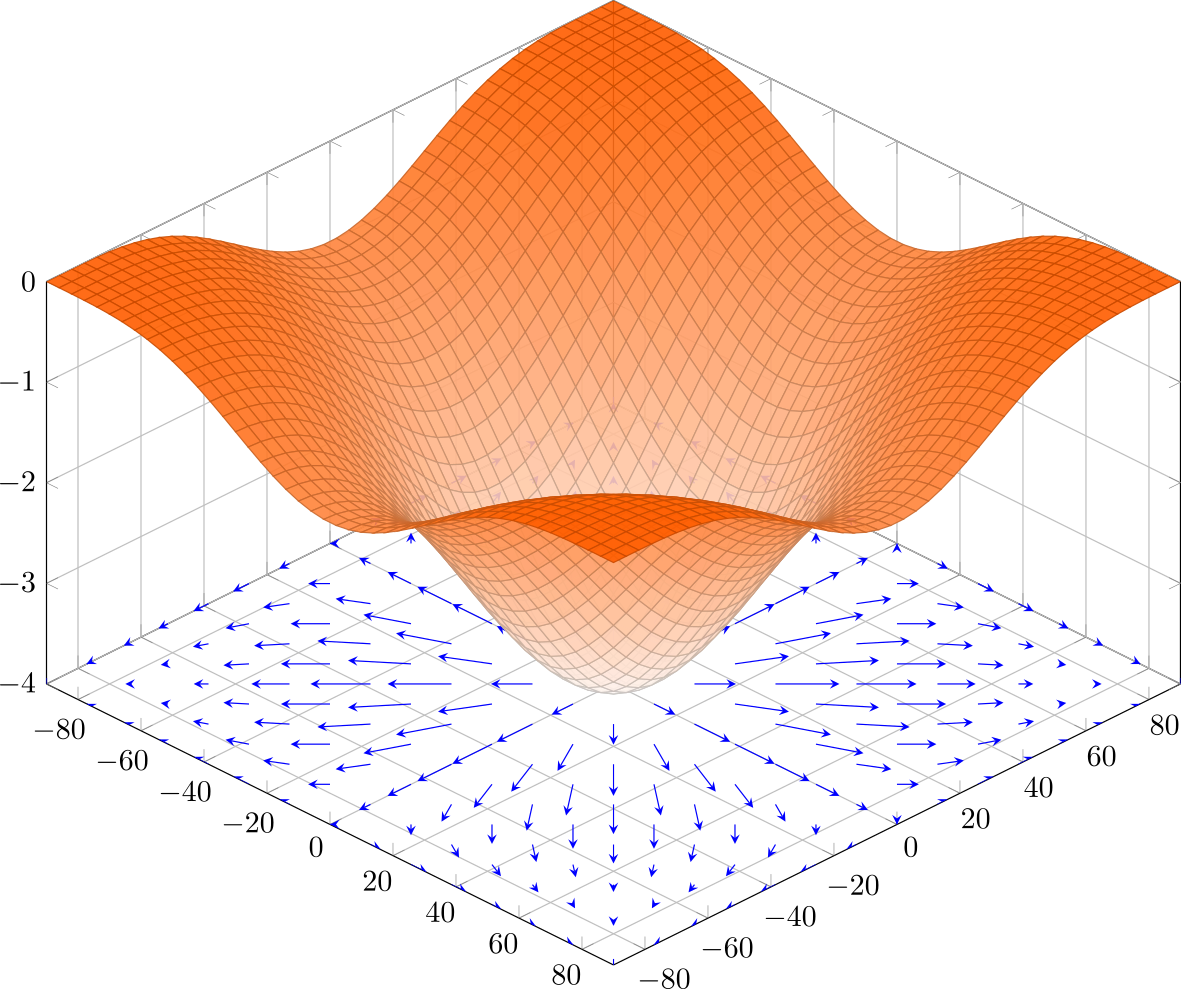
\includegraphics[width=.5\linewidth]{3d-gradient-cos-vector} % Thanks to https://en.wikipedia.org/wiki/Gradient
	\end{center}
	Spesso è comodo identificare $A$ con l'insieme
	\[\brackets{(x,y,z) \in \R^3:\; (x,y) \in A \text{ e } z = 0}\]
	ed in questo caso il gradiente può essere convenzionalmente esteso con una terza coordinata costante $0$.
\end{observation}

\subsection{Il Significato Geometrico del Gradiente}
In questo paragrafo si vedrà la relazione "geometrica" tra il gradiente e la funzione stessa. Il \textbf{Gradiente} di una funzione in un punto indica infatti la direzione in cui si ha la \textbf{massima variazione} del valore di $f$ con \textbf{verso} dell'\textbf{incremento positivo} di $f$.
\begin{proposition}[Significato del Gradiente]
	Siano $A \subseteq \R^2$, $(x_0, y_0) \in \circdot{A}$, $f: A \to \R$ con $f$ \textbf{Differenziabile} in $(x_0, y_0)$.\\
	L'incremento $f(x_0 + h, y_0 + k) - f(x_0, y_0)$ è
	\begin{itemize}[noitemsep]
		\item \textbf{massimo} quando $\begin{bmatrix}h & k\end{bmatrix} = \lambda \nabla f(x_0, y_0)$ con $\lambda > 0$
		\item \textbf{massimo} quando $\begin{bmatrix}h & k\end{bmatrix} = \lambda \nabla f(x_0, y_0)$ con $\lambda < 0$
	\end{itemize}
	Cioè $\nabla f(x_0)$ è un vettore diretto verso la direzione di \textbf{massima pendenza}, "verso l'alto."
	\begin{proof}
		Utilizzando la \fullref{def:differenz}, declinata nel caso $n = 2$ si ottine
		\begin{equation}
			\label{eq:dim_dir_grad}
			f(x_0 + h, y_0 + k) -
			f(x_0, y_0) =
			\nabla f(x_0, y_0) \cdot
			\begin{bmatrix}
				h\\k
			\end{bmatrix} +
			o(\sqrt{h^2 + k^2})
			\qquad \text{ per } (h,k) \to (0,0)
		\end{equation}
		Il $\;\cdot\;$ della precedente formula è un prodotto righe per colonne, però, essendo alla ricerca di un massimo, conviene considerarlo come un prodotto scalare tra due vettori. Il risultato del prodotto scalare è infatti un valore in $\R$, campo ordinabile. Dunque, posto $\theta$ angolo tra i due vettori:
		\[\norm{\nabla f(x_0, y_0)} \norm{\begin{bmatrix}h\\k\end{bmatrix}} \cos(\theta)\]
		Il $\theta$ che massimizza questo prodotto è sicuramente $0$, in quanto $\cos(0) = 1$.\\
		$\nabla f$ dipende direttamente dalla $f$, dunque la sua direzione è data ed inalterabile. D'altro canto $\begin{bmatrix}h\\k\end{bmatrix}$ è un vettore a scelta, dunque la sua direzione è variabile. È possibile allora ottenere una variazione di $\theta$ modificando la direzione di quest'ultimo vettore, finché esso non sarà parallelo al gradiente, portando $\theta$ a $0$.

		Si è così dimostrato che l'incremento $f(x_0 + h, y_0 + k) - f(x_0, y_0)$ da \cref{eq:dim_dir_grad} è massimo quando $h$ ha la direzione del gradiente; dunque il gradiente deve avere direzione e verso del massimo incremento.

		Nel caso in cui si abbia verso opposto $\theta = -180^\circ \implies \cos(\theta) = -1$. Quindi con $\lambda < 0$ si ha minimo incremento.
		\vspace*{\baselineskip}
		\begin{center}
			\begin{tikzpicture}[> = stealth]
				\coordinate (O) at (1,1);
				\coordinate (nabl) at (1.5,5);
				\coordinate (h1) at (4.5,1.5);
				\coordinate (h2) at (3.5,3);

				\draw[thick, ->] (O) -- node[above left] {$\nabla f(x_0)$} (nabl);
				\draw[->] (O) -- node[below] {$h'$} (h1);
				\draw[->] (O) -- node[below] {$h''$} (h2);

				\draw pic["$\theta'$", draw=black!50, -, angle eccentricity=1.2, angle radius=55] {angle=h1--O--nabl};
				\draw pic["$\theta''$", draw=black!50, -, angle eccentricity=1.3, angle radius=25] {angle=h2--O--nabl};

				\node (text_nabl) [align=center] at (4,4.2) {$\nabla f$ ha direzione\\fissa, è unico};
				\draw[thin, ->, shorten >=4pt] (text_nabl.west) to[out=180, in=-20] (nabl);

				\node (text_h) [align=center] at (6.5,2.5) {la direzione di $h$\\varia, se ne possono\\scegliere diversi};
				\draw[thin, ->, shorten >=4pt] (text_h.west) to[out=210, in=80] (h1);
				\draw[thin, ->, shorten >=4pt] (text_h.west) to[out=180, in=-30] (h2);
			\end{tikzpicture}
		\end{center}
	\end{proof}
\end{proposition}
\begin{proposition}[Il Gradiente è Perpendicolare alle Curve di Livello]
	\label{prop:curv_liv_perp_grad}
	Siano $A \subseteq \R^2$, $(x_0, y_0) \in \circdot{A}$ e $f: A \to \R$, se:
	\begin{itemize}
		\item $f$ \textbf{Differenziabile} in $(x_0, y_0)$
		\item $(x_0, y_0)$ \textbf{non Stazionario}
	\end{itemize}
	Allora
	\[\nabla f(x_0, y_0) \text{ è \textbf{Perpendicolare} alla \textbf{Curva di Livello} } \brackets{(x,y) \in A:\; f(x,y) = c}\]
	\begin{proof}
		Essendo, per ipotesi, $(x_0, y_0)$ non Stazionario, da \fullref{def:pto_staz} si sa per certo che $\nabla f(x_0, y_0) \neq 0$, cioè
		\[
			\begin{gathered}
				\nabla f(x_0, y_0) \neq 0\\
				\iff\\
				\begin{bmatrix}
					\partial_x f(x_0, y_0) & \partial_y f(x_0, y_0)
				\end{bmatrix}
				\neq 0\\
				\iff\\
				\partial_x f(x_0, y_0) \neq 0 \quad \text{oppure} \quad \partial_y f(x_0, y_0) \neq 0
			\end{gathered}
		\]
		Si supponga dunque $\partial_y f(x_0,y_0) \neq 0$ ed applicando il \fullref{teo:funz_impl} si ha che esistono degli intorni $\mathcal{X}$ di $x_0$ e $\mathcal{Y}$ di $y_0$ e, per $x \in \mathcal{X}$ e $y \in \mathcal{Y}$, esiste la
		\[\varphi: \mathcal{X} \to \mathcal{Y} \quad \text{tale che} \quad f(x,y) = 0 \iff y = \varphi(x)\]
		\vspace*{-\baselineskip}
		\begin{note}
			Verifica ipotesi:
			\begin{enumerate}
				\item $A \subseteq \R \times \R$ e, per ipotesi, $(x_0, y_0) \in \circdot{A}$. Essendo un punto della parte interna la condizione è verificata perché nel \fullref{teo:funz_impl} l'apertura di $X$ e $Y$ è richiesta solo per scegliere un punto, appunto, sicuramente nella parte interna degli insiemi
				\item $f \in \cntclass{1}$ per ipotesi, quindi sicuramente continua
				\item $(x_0, y_0) \in A$ per ipotesi e la funzione da invertire vale $0$ perché, anche se fosse $f(x_0, y_0) = c \neq 0$, è sempre possibile utilizzare una funzione $g(x_0, y_0) = f(x_0, y_0) - c = 0$ che verifica questa ipotesi e per cui valgono ancora tutte le altre osservazioni fatte qui
				\item $f$ differenziabile in $(x_0, y_0)$ per ipotesi, dunque sicuramente esiste $\partial_y f$
				\item $D_yf(x_0, y_0)$ ammette inversa perché è stato ipotizzato $\partial_y f(x_0,y_0) \neq 0$ poco sopra
			\end{enumerate}
		\end{note}
		La $y = \varphi(x)$ quindi esprime implicitamente il vincolo della curva di livello $f(x, y) = c$. È dunque possibile scrivere, separando le coordinate e passando alla matrice associata:
		\[
			f(x, y) = c \quad \iff \quad y = \varphi(x) \quad \iff \quad
			\begin{bmatrix}
				x\\
				\varphi(x)
			\end{bmatrix}
		\]
		Visto che il differenziale di una funzione in un puno rappresenta il versore tangente alla funzione in quel punto, si passa alle derivate $\begin{bmatrix}1\\\varphi'(x)\end{bmatrix}$, visto che valgono anche le ipotesi del \fullref{teo:funz_impl_diff}. Eseguendo ora il prodotto tra $\nabla f(x_0, y_0)$ e la derivate nel punto $(x_0, y_0)$, si ottiene
		\begin{align*}
			\lefteqn{\nabla f(x_0, y_0) \cdot \begin{bmatrix}1\\\varphi'(x_0)\end{bmatrix} =}\\
			&= \begin{bmatrix}
				\partial_x f(x_0, y_0) & \partial_y f(x_0, y_0)
			\end{bmatrix}
			\cdot
			\begin{bmatrix}
				1\\
				-\frac{\partial_x f(x_0, y_0)}{\partial_y f(x_0, y_0)}
			\end{bmatrix} =\\
			&= \partial_x f(x_0, y_0) - \partial_x f(x_0, y_0)\\
			&= 0
		\end{align*}
		Dunque, considerando questo come un prodotto scalare, se il risultato è $0$ allora l'angolo tra i due vettori non può che essere $90^\circ$, da cui la tesi.
	\end{proof}
\end{proposition}
\begin{definition}[Piano Tangente ad una Curva]
	Siano $A \subseteq \R^2$, $(x_0, y_0) \in \circdot{A}$, $f: A \to \R$ e $f \in \cntclass{1}(A; \R)$, allora l'\textbf{Equazione del Piano Tangente} alla curva nel punto $(x_0, y_0)$ è:
	\begin{align*}
		z &= f(x_0, y_0) + \nabla f(x_0, y_0) \begin{bmatrix}x - x_0\\y - y_0\end{bmatrix}\\
		&= f(x_0, y_0) + \partial_x f(x_0, y_0) (x - x_0) + \partial_y f(x_0, y_0) (y - y_0)
	\end{align*}
	Passando alla matrice associata si ottiene la forma del vettore \textbf{Perpendicolare} alla curva in $(x_0, y_0)$, cioè:
	\[
		\begin{bmatrix}
			\partial_x f(x_0, y_0)\\
			\partial_y f(x_0, y_0)\\
			-1
		\end{bmatrix}
	\]
\end{definition}

\subsection{I Moltiplicatori di Lagrange}
Il seguente teorema è una versione più specifica del \fullref{teo:molt_lagr_gen}, dunque molte note sono omesse in questo enunciato.
\begin{theorem}[dei Moltiplicatori di Lagrange - $n=2$, $m=1$]
	\label{teo:molt_lagr_n2_m1}
	Sia $A \subseteq \R^2$ un \textbf{Aperto} e siano
	\begin{itemize}[noitemsep]
		\item $f: A \to \R$
		\item $\varphi: A \to \R$ con $\varphi^{-1}(0) \subset A$
	\end{itemize}
	due funzioni $\in \cntclass{1}$.
	Se:
	\begin{itemize}[noitemsep]
		\item $(x_0, y_0)$ è un punto di \textbf{estremo relativo} per $f$ \textbf{vincolata} a $\varphi = 0$
		\item $\nabla \varphi(x_0, y_0) \neq 0$
	\end{itemize}
	Allora esiste un $\lambda$ tale che
	\begin{equation}
		\nabla f(x_0, y_0) = \lambda \nabla \varphi(x_0, y_0)
	\end{equation}
	Lo scalare $\lambda$ è chiamato \textbf{Moltiplicatore di Lagrange}.
	\begin{proof}~
		\begin{note}
			Questa dimostrazione è molto simile alla soluzione dell'\fullref{ex:molt_lagr_sist_equiv}.
		\end{note}
		Essendo per ipotesi $\nabla \varphi(x_0, y_0) \neq 0$, allora
		\[
			\begin{gathered}
				\nabla \varphi(x_0, y_0) \neq 0\\
				\iff\\
				\begin{bmatrix}
					\partial_x \varphi(x_0, y_0) & \partial_y \varphi(x_0, y_0)
				\end{bmatrix}
				\neq 0\\
				\iff\\
				\partial_x \varphi(x_0, y_0) \neq 0 \quad \text{oppure} \quad \partial_y \varphi(x_0, y_0) \neq 0
			\end{gathered}
		\]
		Si supponga dunque $\partial_y \varphi(x_0,y_0) \neq 0$ ed applicando il \fullref{teo:funz_impl} si ha che esistono degli intorni $\mathcal{X}$ di $x_0$ e $\mathcal{Y}$ di $y_0$ e, per $x \in \mathcal{X}$ e $y \in \mathcal{Y}$, esiste la
		\[g: \mathcal{X} \to \mathcal{Y} \quad \text{tale che} \quad \varphi(x,y) = 0 \iff y = g(x)\]
		\vspace*{-\baselineskip}
		\begin{note}
			Verifica ipotesi:
			\begin{enumerate}
				\item $A \subseteq \R \times \R$ aperto per ipotesi
				\item $f \in \cntclass{1}$ per ipotesi, quindi sicuramente continua
				\item $(x_0, y_0) \in A$ per ipotesi e la funzione da invertire vale $0$ perché, anche se fosse $f(x_0, y_0) = c \neq 0$, è sempre possibile utilizzare una funzione $g(x_0, y_0) = f(x_0, y_0) - c = 0$ che verifica questa ipotesi e per cui valgono ancora tutte le altre osservazioni fatte qui
				\item $f$ differenziabile in $(x_0, y_0)$ per ipotesi, dunque sicuramente esiste $\partial_y f$
				\item $D_yf(x_0, y_0)$ ammette inversa perché è stato ipotizzato $\partial_y f(x_0,y_0) \neq 0$ poco sopra
			\end{enumerate}
		\end{note}
		Definendo la $F(x) = f \bigl( x, g(x) \bigr)$, i punti di estremo della $f$ vincolata a $\varphi$ saranno di estremo anche per $F$ a patto di rimanere in un intorno di $(x_0, y_0)$ in cui vale il \fullref{teo:funz_impl}.\\
		$F$ è differenziabile ovunque definita, visto che $f \in \cntclass{1}$ per ipotesi, quindi per il \fullref{teo:fermat}, se $(x_0, y_0)$ è di estremo, allora $F'(x_0, y_0) = 0$.
		\begin{note}
			Essendo $F: \R \to \R$ si può usare la notazione $F'$ della derivata di Analisi 1.
		\end{note}
		Calcolando ora $F'(x_0)$ grazie alla \fullref{prop:deriv_funz_comp}
		\begin{align*}
			0
			&= F'(x_0)\\
			&=	\partial_x f\bigl( x_0, g(x_0) \bigr) +
				\partial_y f\bigl( x_0, g(x_0) \bigr) \cdot
				g'(x_0)\\
			&=	\partial_x f\bigl( x_0, g(x_0) \bigr) +
				\partial_y f\bigl( x_0, g(x_0) \bigr) \cdot
				\left(
					-
					\frac{
						\partial_x g(x_0,g(x_0))
					}{
						\partial_y g(x_0,g(x_0))
					}
				\right)\\
			&=	\partial_x f\bigl( x_0, g(x_0) \bigr) \cdot \partial_y g(x_0,g(x_0)) -
				\partial_y f\bigl( x_0, g(x_0) \bigr) \cdot \partial_x g(x_0,g(x_0))
			\shortintertext{Che può essere rappresentato in forma compatta come il $\det$ di una matrice $\mat (2 \times 2)$}
			&=	\det \left(
				\begin{matrix}
					\partial_xf(x_0,y_0) & \partial_yf(x_0,y_0)\\
					\partial_xg(x_0,y_0) & \partial_yg(x_0,y_0)
				\end{matrix}
				\right)
		\end{align*}
		Prendendo il primo e l'ultimo elemento del treno di uguaglianze si ha che $\det = 0$, dunque, dalle nozioni di Algebra, si sa che questo implica il parallelismo tra i vettori della matrice. Essendo la $g$ e la $\varphi$ legate implicitamente, è possibile concludere che:
		\[\exists \lambda \in \R: \nabla f(x_0,y_0) = \lambda \nabla \varphi(x_0,y_0)\]
	\end{proof}
\end{theorem}
\begin{exercise}
	Dimostrare la \fullref{teo:molt_lagr_n2_m1} nel caso in cui $\partial_x \varphi(x_0, y_0) \neq 0$ e $\partial_y \varphi(x_0, y_0) = 0$
	\begin{solution}
		È sufficiente applicare il \fullref{teo:funz_impl} alla $\partial_x$, gli altri passaggi non variano.
	\end{solution}
\end{exercise}
\begin{exercise}
	Dare un'interpretazione geometrica della \fullref{teo:molt_lagr_n2_m1} in luce della \fullref{prop:curv_liv_perp_grad}.
	\begin{solution}
		Fornita in \fullref{obs:concetto_teo_molt_lagr_gen}.
	\end{solution}
\end{exercise}
\begin{exercise}
	Nel piano, determinare il punto della retta passante per $(-1, 2)$ $(1, 4)$ più vicino alla circonferenza centrata in $(0, 0)$ di raggio $2$. Utilizzare la \fullref{sect:geom_piano}.
\end{exercise}
\begin{exercise}
	Nel piano, determinare il punto della circonferenza centrata in $(0, 0)$ di raggio $3$ più lontano dalla retta passante per $(1, 2)$ $(1, -1)$. Utilizzare la \fullref{sect:geom_piano}.
\end{exercise}

\newpage
\cbstart
\section{Derivate e Integrali}
\begin{theorem}[Fondamentale del Calcolo Integrale]
	\label{teo:fondament_calcolo_integ}
	Sia $I\subseteq \R$ un \textbf{Intervallo} e sia $x_0\in I$. Data $f\in \cntclass{0}(I;R)$ la funzione:
	\[\funcdef{F}{I}{\R}{x}{\displaystyle\int_{x_0}^{x}f(t)\integrald{t}}\]
	Si ha $F\in \cntclass{1}(I;\R)$ e $F'(x)=f(x) \quad \forall x \in I$
	\begin{proof}
		Omessa. Vedasi corso di Analisi 1.
	\end{proof}
\end{theorem}
\begin{proposition}
	\label{prop:f_C0_allora_F_C0}
	Siano $A \subseteq \R^n$ un \textbf{Aperto} e $f \in \cntclass{0}(A \times \R;\R)$, allora la funzione
	\[\funcdef{F}{\R \times \R \times A}{\R}{\alpha, \beta, x}{\displaystyle\int_{\alpha}^{\beta} f(x,t)\integrald{t}}\]
	è di classe $\cntclass{0}(\R \times \R \times A;\R)$
	\begin{proof}
		La continuità di $F$ rispetto ad $\alpha$ e $\beta$ segue dal \fullref{teo:fondament_calcolo_integ}.\\
		Per verificare la continuità di $F$ in $x_0 \in A$, si scelga un $r > 0$ tale per cui $\overline{B(x_0, r)} \subset A$. La $f$ sarà continua in $\overline{B(x_0, r)} \times \intervalclose{\alpha}{\beta}$, in quanto, per ipotesi:
		\[f \in \cntclass{0}(\underbrace{A}_{\overline{B(x_0, r)} \subset A} \times \underbrace{\R}_{\intervalclose{\alpha}{\beta} \subset \R};\R)\]
		Inoltre, da \fullref{prop:compat_chius_lim_Rn} si ottiene che $\overline{B(x_0, r)} \times \intervalclose{\alpha}{\beta}$ è compatto. Per questo è possibile applicare il \fullref{teo:cantor} ed avere certezza che la $f$ è \fullref{def:funz_unif_cont} in quell'intervallo. Dalla definizione e passando alla metrica Euclidea in $\R^2$ si può desumere che:
		\[\forall \varepsilon > 0 \quad \exists \delta > 0 \text{ tale che } \forall x,x_0 \in \brackets{\overline{B(x_0, r)} \times \intervalclose{\alpha}{\beta}} \text{ con } \abs{x - x_0} < \delta \quad \text{vale } \abs{f(x, t) - f(x_0, t)} < \varepsilon\]
		Dunque, sicuramente, passando al $\sup$ resta valido che
		\begin{equation}
			\label{eq:deriv_integ_F_alfa_beta_C0}
			\sup\limits_{\overline{B(x_0, r)} \times \intervalclose{\alpha}{\beta}} \underbrace{\abs{f(x, t) - f(x_0, t)} < \varepsilon}_{\text{(1)}}
		\end{equation}
		A questo punto, utilizzando la definizione di $F$ ci si riconduce ad una forma simile alla (1):
		\begin{align*}
			\abs{F(\alpha, \beta, x) - F(\alpha, \beta, x_0)} &= \abs{\int_{\alpha}^{\beta} f(x,t)-f(x_0, t) \integrald{t}}
			\shortintertext{Grazie all'osservazione di \fullref{ex:cau_loc_abs_of_norm} è possibile minorare}
			&\leq  \abs{\int_{\alpha}^{\beta} \abs{f(x,t)-f(x_0, t)} \integrald{t}}
			\shortintertext{Applicando la \cref{eq:deriv_integ_F_alfa_beta_C0}}
			&< \abs{\int_{\alpha}^{\beta} \varepsilon \integrald{t}}
			\shortintertext{Per integrale di funzione costante, infine}
			&= (\beta - \alpha) \varepsilon
		\end{align*}
		Quindi, riprendendo il primo e l'ultimo termine:
		\[\abs{F(\alpha, \beta, x) - F(\alpha, \beta, x_0)} < (\beta - \alpha) \varepsilon\] % WARNING Sul libro c'è un <= ma prima si è dimostrata una minorazione stretta e questa è necessaria per la dimostrazione stessa, dunque usare <= è sbagliato
		che dà la tesi, in quanto si ha la distanza tra le $F$ minorata strettamente da un qualsiasi $\varepsilon > 0$, per cui la distanza deve necessariamente essere nulla.
	\end{proof}
\end{proposition}
\begin{proposition}
	\label{prop:f_C1_allora_F_C1}
	Siano $A \subseteq \R^n$ un \textbf{Aperto} e $f \in \cntclass{1}(A \times \R;\R)$, allora la funzione
	\[\funcdef{F}{\R \times \R \times A}{\R}{\alpha, \beta, x}{\displaystyle\int_{\alpha}^{\beta} f(x,t)\integrald{t}}\]
	è di classe $\cntclass{1}(\R \times \R \times A;\R)$ ed inoltre, per ogni $(\alpha, \beta, x) \in \R \times \R \times A$ e per ogni $i = 1,\:\dotsc\:,n$ si ha
	\begin{align*}
		\partial_\alpha F(\alpha, \beta, x) \quad &= \quad -f(x, \alpha)\\
		\partial_\beta F(\alpha, \beta, x) \quad &= \quad f(x, \beta)\\
		\partial_{x_i} F(\alpha, \beta, x) \quad &= \quad \int_{\alpha}^{\beta} \partial_{x_i} f(x,t) \integrald{t}\\
		\nabla F(\alpha, \beta, x) \quad &= \quad \int_{\alpha}^{\beta} \nabla f(x,t) \integrald{t}
	\end{align*}
	\begin{proof}
		Le prime due uguaglianza seguono direttamente dal \fullref{teo:fondament_calcolo_integ}.\\
		Per dimostrare la terza si segue un procedimento analogo a quello di \fullref{prop:f_C0_allora_F_C0}: si scelga un $r > 0$ tale per cui $\overline{B(x_0, r)} \subset A$. Essendo $f \in \cntclass{1}$, allora sicuramente $\partial_{x_i} f \in \cntclass{0}$, dunque come dall'altra dimostrazione, $\partial_{x_i} f$ sarà Uniformemente Continua in $\overline{B(x_0, r)} \times \intervalclose{\alpha}{\beta}$. Grazie a questo si sa che:
		\[\forall \varepsilon > 0 \quad \exists \delta > 0 \text{ tale che } \forall x,x_0 \in \brackets{\overline{B(x_0, r)} \times \intervalclose{\alpha}{\beta}} \text{ con } \abs{x - x_0} < \delta \quad \text{vale } \abs{\partial_{x_i} f(x, t) - \partial_{x_i} f(x_0, t)} < \varepsilon\]
		Dunque, sicuramente, passando al $\sup$ resta valido che
		\begin{equation}
			\label{eq:deriv_integ_F_alfa_beta_C1}
			\sup\limits_{\overline{B(x_0, r)} \times \intervalclose{\alpha}{\beta}} \underbrace{\abs{\partial_{x_i} f(x, t) - \partial_{x_i} f(x_0, t)} < \varepsilon}_{\text{(1)}}
		\end{equation}
		A questo punto, utilizzando si riconduce la terza uguaglianza ad una forma simile alla (1) spostando il termine di destra al primo membro e calcolanone il valore assoluto:
		\begin{align*}
			&\abs{
				\partial_{x_i} F(\alpha, \beta, x) -
				\int_{\alpha}^{\beta} \partial_{x_i} f(x,t) \integrald{t}
			} =
			\shortintertext{Applicando la \fullref{def:deriv_direz} ad una qualsiasi $x_i$, dunque con $v = h e_i$ per uno qualsiasi dei vettori della base canonica}
			= &\abs{
				\frac{F(\alpha, \beta, x + h e_i) - F(\alpha, \beta, x)}{h} -
				\int_{\alpha}^{\beta} \partial_{x_i} f(x,t) \integrald{t}
			}
			\shortintertext{Applicando ora la definizione di $F$ e portando il denominatore dentro il segno d'integrale}
			= &\abs{
				\int_{\alpha}^{\beta} \frac{f(x + h e_i, t) - f(x, t)}{h} \integrald{t} -
				\int_{\alpha}^{\beta} \partial_{x_i} f(x,t) \integrald{t}
			}\\
			= &\abs{
				\int_{\alpha}^{\beta} \left(
					\underbrace{\frac{f(x + h e_i, t) - f(x, t)}{h}}_{\text{(1)}} - \partial_{x_i} f(x,t)
				\right) \integrald{t}
			}
			\shortintertext{Considerando ora la (1) come una funzione in $x$, le si può applicare il \fullref{teo:lagrange} e per un certo $\theta \in \intervalopen{0}{1}$ si ha che}
			= &\abs{
				\int_{\alpha}^{\beta} \Bigl(
					\partial_{x_i} f(x + \theta h e_i, t) - \partial_{x_i} f(x,t)
				\Bigr) \integrald{t}
			}
			\shortintertext{Grazie all'osservazione di \fullref{ex:cau_loc_abs_of_norm} è possibile minorare}
			\leq &\abs{
				\int_{\alpha}^{\beta} \Bigl| % Not using \abs notation since the | were too short and could have been missed out reading quickly
					\partial_{x_i} f(x + \theta h e_i, t) - \partial_{x_i} f(x,t)
				\Bigr| \integrald{t}
			}
			\intertext{Applicando la \cref{eq:deriv_integ_F_alfa_beta_C1} e ricordando che $h = x - x_0$, si sa che se $\abs{h} < \delta$, sicuramente anche $\abs{\theta h} < \delta$ in quanto $\theta \in \intervalopen{0}{1}$, dunque}
			&< \abs{\int_{\alpha}^{\beta} \varepsilon \integrald{t}}
			\shortintertext{Per integrale di funzione costante, infine}
			&= (\beta - \alpha) \varepsilon
		\end{align*}
		Quindi, riprendendo il primo e l'ultimo termine:
		\[\abs{\partial_{x_i} F(\alpha, \beta, x) - \int_{\alpha}^{\beta} \partial_{x_i} f(x,t) \integrald{t}} < (\beta - \alpha) \varepsilon\] % WARNING Sul libro c'è un <= ma prima si è dimostrata una minorazione stretta e questa è necessaria per la dimostrazione stessa, dunque usare <= è sbagliato
		da cui la tesi, in quanto si ha la distanza tra le due funzioni minorata strettamente da un qualsiasi $\varepsilon > 0$, per cui la distanza deve necessariamente essere nulla.\\
		La quarta uguaglianza è diretta conseguenza della terza appena dimostrata.

		La continuità delle derivate parziali segue dalla \fullref{prop:f_C0_allora_F_C0}, dunque grazie al \fullref{teo:diff_tot} $F \in \cntclass{1}$.
	\end{proof}
\end{proposition}
\begin{corollary}
	Siano $A \subseteq \R^n$ un \textbf{Aperto}. Date le funzioni
	\begin{itemize}[noitemsep]
		\item $\alpha:\; A \to \R$
		\item $\beta:\; A \to \R$
		\item $f:\; A \times \R \to \R$
	\end{itemize}
	\textbf{tutte} di classe $\cntclass{1}$, allora la funzione
	\[\funcdef{F}{A}{\R}{x}{\displaystyle\int_{\alpha(x)}^{\beta(x)} f(x,t)\integrald{t}}\]
	è di classe $\cntclass{1}$ ed inoltre, per ogni $x_0 \in A$ si ha
	\[
		\nabla F(x_0) =
		f \bigl( x_0, \beta(x_0) \bigr) \nabla \beta(x_0) -
		f \bigl( x_0, \alpha(x_0) \bigr) \nabla \alpha(x_0) +
		\int_{\alpha(x_0)}^{\beta(x_0)} \nabla f(x_0, t) \integrald{t}
	\]
	\begin{proof}
		Immediata applicando la \fullref{prop:f_C1_allora_F_C1} e la \fullref{prop:deriv_funz_comp}.
	\end{proof}
\end{corollary}
\cbend

\newpage
\section{Funzioni a Valori in \texorpdfstring{$\protect\C$}{C}}\label{sect:fun_in_C}
Sia $A \subseteq \R^n$ non vuoto. Ogni funzione $A \to \C$ può essere identificata in modo naturale con una funzione $A \to \R^2$ e viceversa.
\begin{note}
	Quindi è possibile rappresentare una funzione $A \to \C$ in un piano, detto \textbf{piano complesso} o \textbf{piano di Gauss}
\end{note}
\begin{exercise}
	\label{ex:ext_def_in_C}
	Utilizzando questa identificazione, estendere al caso di funzioni $A \to \C$ le definizioni di continuità, derivabilità, differenziabilità e degli spazi $\cntclass{k}$ date per funzioni $A \to \R$
	% TODO solution
\end{exercise}
\begin{proposition}
	\label{prop:fg_in_C}
	Sia $A \subseteq \R$ e sia $t_0 \in \circdot{A}$. Allora
	\begin{itemize}
		\item Se due funzioni $f,g: A \to \C$ sono differenziabili in $t_0$, anche le funzioni $f+g$ e $f \cdot g$ sono differenziabili in $t_0$. Inoltre
			\[(f+g)'(t_0) = f'(t_0) + g'(t_0) \qquad\text{e}\qquad (f \cdot g)'(t_0) = f'(t_0)g(t_0)+f(t_0)g'(t_0)\]
		\item Per ogni $\lambda \in \C$, anche $\lambda f$ è differenziabile e
			\[(\lambda f)'(t_0) = \lambda f'(t_0)\]
		\item Se $g(t_0) \neq 0$, anche $1/g$ e $f/g$ sono differenziabili in $t_0$ e
			\[(1/g)'(t_0) = - \frac{g'(t_0)}{g^2(t_0)} \qquad\text{e}\qquad (f/g)'(t_0) = \frac{f'(t_0)g(t_0)-f(t_0)g'(t_0)}{g^2(t_0)}\]
	\end{itemize}
	\begin{proof}
		Omessa
	\end{proof}
\end{proposition}
\begin{exercise}
	Dimostrare la \fullref{prop:fg_in_C}
	% TODO solution
\end{exercise}
\begin{definition}[Funzione Esponenziale con Esponente Complesso]
	\label{def:exp_complesso}
	La Funzione Esponenziale con Esponente Complesso è così definita:
	\[e^{x+iy} = e^x \cdot (\cos y + i \sin y)\]
\end{definition}
\begin{proposition}
	\label{prop:deriv_exp_in_C}
	Qualunque sia $\lambda \in \C$,
	\[\frac{d}{dt}e^{\lambda t} = \lambda e^{\lambda t}\]
	\begin{proof}
		Omessa
	\end{proof}
\end{proposition}
\begin{exercise}
	Dimostrare la \fullref{prop:deriv_exp_in_C}, direttamente o attraverso l'\fullref{ex:deriv_func_with_taylor}
\end{exercise}
\begin{exercise}
	In questa sezione sulle funzioni a valori complessi non son stati considerati i problemi di massimo/minimo, perché?
	\begin{solution}
		Perché $\C$ non è ordinato, dunque non è possibile trovare massimi o minimi.
	\end{solution}
\end{exercise}